%----------------------------------------------------------------------------------------------------------------------------
\graphicspath{{Parti/P04-Travi_rigide/C05-Sistemi_reticolari/Figure/}}
\chapter{Sistemi reticolari}
\label{cap:reticolari}
%----------------------------------------------------------------------------------------------------------------------------

\begin{sommario}
	Si sviluppano i metodi di analisi delle travature
	reticolari piane. Si introduce la doppia lettura
	topologica --- aste come corpi rigidi o nodi come
	protagonisti --- e se ne ricava la formula di
	M\"{u}ller-Breslau con il principio di composizione
	gerarchica come procedura costruttiva che garantisce
	l'isostaticità.
	Sul versante cinematico si distingue la
	sovradeterminazione esterna da quella interna
	e si analizzano gli effetti di cedimenti e
	distorsioni, introducendo il polo dell'asta
	come strumento di lettura.
	Sul versante statico si sviluppano il metodo
	dei nodi e il metodo delle sezioni di Ritter,
	con l'analogia della trave equivalente per le
	travature a correnti paralleli.
	Si tratta il caso delle aste con carichi
	trasversali e si inquadra la struttura della
	soluzione per le travature iperstatiche,
	rinviando al Vol.~II per la determinazione
	delle incognite iperstatiche.
\end{sommario}




\section*{Considerazioni introduttive}
\label{sec:raccordo_reticolari}

Nel \CAPref{cap:assemblaggi_travi} le travature reticolari
sono state inquadrate nel catalogo delle tipologie
strutturali, anticipando che la connessione esclusivamente
a cerniera, quando i carichi agiscono ai nodi, riduce
lo stato di sollecitazione di ciascuna asta al solo
sforzo normale, eliminando taglio e momento flettente.
Questa proprietà --- che distingue i sistemi reticolari
da tutte le altre tipologie strutturali --- non è solo
una semplificazione analitica: è il principio che rende
le travature reticolari la soluzione d'elezione per
coprire grandi luci con un impiego efficiente del
materiale, concentrando la resistenza dove serve,
nei correnti tesi e compressi, e affidando alla parete
il solo compito di trasferire i carichi ai nodi.
Il presente capitolo ne sviluppa i fondamenti e i
metodi di analisi cinematica e statica.

%----------------------------------------------------------------------------------------------------------------------------
\section{Doppia lettura topologica.}
\label{sec:doppia_lettura}
%----------------------------------------------------------------------------------------------------------------------------
Un \emph{sistema reticolare}\index{sistema reticolare|textbf} è un sistema di travi
rettilinee --- dette \emph{aste}\index{asta|textbf} --- collegate
esclusivamente mediante cerniere interne e vincolato
al suolo esclusivamente mediante cerniere e carrelli.

Nella teoria generale dei sistemi di corpi rigidi
sviluppata nella Parte~II, le travi sono i
protagonisti e le connessioni sono i vincoli.
Nei sistemi reticolari questa prospettiva rimane
valida --- ed è la \emph{prima lettura} --- ma
ammette una lettura alternativa, la
\emph{seconda lettura}\index{lettura topologica!seconda}, in cui i punti di
connessione --- i \emph{nodi a cerniera}\index{nodo!di reticolo|textbf} ---
diventano i protagonisti e le aste diventano
i vincoli. Il passaggio da una lettura all'altra
è reso possibile da una proprietà geometrica
peculiare delle cerniere: la rotazione di ogni
asta è univocamente determinata dalle posizioni
dei due nodi di estremità e non è quindi un
grado di libertà indipendente del sistema.

\begin{itemize}[noitemsep]
	\item \emph{Prima lettura --- aste come corpi
		rigidi}: le aste sono i protagonisti, le cerniere
	sono i connettori. Ogni asta contribuisce con
	$n = 3$ gradi di libertà (due traslazioni e una
	rotazione); ogni cerniera interna tra $e_i$ aste
	convergenti impone $m_i = 2(e_i-1)$ equazioni
	di congruenza (uguaglianza degli spostamenti
	traslazionali). Per dualità $\bm{B}=\bm{A}^\top$,
	il problema statico ha come variabili le reazioni
	delle cerniere interne --- due componenti per
	ciascuna cerniera --- e le reazioni dei vincoli
	esterni, con le equazioni di equilibrio delle
	singole aste come equazioni duali delle condizioni
	di congruenza.
	
	\item \emph{Seconda lettura --- nodi come
		protagonisti}: i nodi a cerniera sono i
	protagonisti, le aste sono i vincoli. Ogni nodo
	a cerniera è un punto geometrico e possiede
	pertanto $2$ gradi di libertà traslazionali,
	senza alcuna rotazione propria; ogni asta impone
	$1$ equazione di vincolo scalare ---
	l'inestensibilità\index{inestensibilita@inestensibilità} --- tra i due nodi che connette.
	Per dualità, il problema statico ha come variabili
	i soli sforzi normali $N_e$ nelle aste e le
	reazioni vincolari esterne, con le equazioni di
	equilibrio nodale --- due proiezioni per ciascun
	nodo libero --- come equazioni duali.
\end{itemize}


\begin{oss}[Perché la rotazione delle aste non è
	un grado di libertà indipendente]\label{oss:rotazione_asta}
	Nella teoria generale dei sistemi di corpi rigidi
	ogni corpo rigido piano possiede tre gradi di
	libertà: due traslazioni e una rotazione.
	Applicando questo conteggio a un sistema
	reticolare con $n_a$ aste si otterrebbero
	$3n_a$ gradi di libertà complessivi.
	Tuttavia, se sono note le posizioni finali dei
	due nodi di estremità, $A' = A + \mathbf{u}_A$ e
	$B' = B + \mathbf{u}_B$, l'orientamento dell'asta
	è univocamente determinato dalla direzione del
	vettore $\overrightarrow{A'B'}$:
	la rotazione è una \emph{grandezza derivata}
	dalle posizioni nodali, non un parametro
	indipendente. Le cerniere consentono rotazioni
	relative tra aste diverse, ma non rendono la
	rotazione di ciascuna asta un grado di libertà
	autonomo del sistema. Ne segue che la seconda
	lettura --- con $2n_n$\nomenclature[L]{$n_n$}{numero di nodi della travatura} gradi di libertà nodali
	e $n_a$ equazioni di inestensibilità --- è non
	solo equivalente alla prima, ma è quella che
	coglie in modo diretto la struttura cinematica
	del sistema.
\end{oss}


%----------------------------------------------------------------------------------------------------------------------------
\section{Formula di M\"{u}ller-Breslau e fonti di sovradeterminazione}
\label{sec:muller_breslau_classificazione}
%----------------------------------------------------------------------------------------------------------------------------

Le due letture topologiche sono algebricamente
equivalenti e conducono allo stesso indice di
classificazione $\nu$. Nella prima lettura si
applica direttamente la formula generale dei
sistemi di corpi rigidi:
\[
\nu = 3n_a - m_{\text{int}} - m_{\text{est}},
\]
dove $m_{\text{int}}$ è la molteplicità complessiva
delle cerniere interne. Nella seconda lettura,
sfruttando il fatto che ogni nodo a cerniera è un
punto geometrico con soli $2$ gradi di libertà
traslazionali e ogni asta impone $1$ equazione di
inestensibilità, la stessa formula si riduce alla
\emph{formula di M\"{u}ller-Breslau}\index{formula di Muller-Breslau@formula di Müller-Breslau|textbf}:
\begin{equation}\label{eq:muller_breslau}
	\nu = 2n_n - n_a - m_{\text{est}}.
\end{equation}
Il sistema è isostatico per $\nu = 0$, labile per
$\nu > 0$, iperstatico per $\nu < 0$.
La seconda forma è quella operativamente più
comoda: richiede solo il conteggio di nodi, aste
e vincoli esterni, senza entrare nel dettaglio
della topologia delle cerniere interne.

%%%%%%%%%%%%%%%%%%%%%%%%%%%%%%%%%%%%%%%%%%%
\begin{figure}[htbp]
	\centering
	\begin{tikzpicture}[
		scale=1.0,
		asta/.style={line width=1.2pt, line cap=round, line join=round, black},
		nodo/.style={circle, fill=white, draw=black,
			inner sep=0pt, minimum size=6pt, line width=1.2pt},
		etasta/.style={circle, draw=black, fill=white,
			inner sep=1pt, font=\scriptsize, line width=0.6pt},
		]
		\coordinate (N1) at (0,   0);
		\coordinate (N2) at (2,   0);
		\coordinate (N3) at (4,   0);
		\coordinate (N4) at (6,   0);
		\coordinate (N5) at (1,   1.6);
		\coordinate (N6) at (3,   1.6);
		\coordinate (N7) at (5,   1.6);
		
		\draw[asta](N1)--(N5);
		\draw[asta](N2)--(N5);
		\draw[asta](N2)--(N6);
		\draw[asta](N3)--(N6);
		\draw[asta](N3)--(N7);
		\draw[asta](N4)--(N7);
		\draw[asta](N1)--(N2)--(N3)--(N4);
		\draw[asta](N5)--(N6)--(N7);
		
		%% Cerniera in N1
		\draw[line width=1.0pt](N1)--++(-0.24,-0.40)--++(0.48,0)--cycle;
		\draw[line width=1.0pt](-0.34,-0.40)--(0.34,-0.40);
		\foreach \x in {-0.28,-0.14,0.00,0.14,0.28}
		\draw[very thin](\x,-0.40)--++(-.10,-0.13);
		
		%% Carrello in N4
		\draw[line width=1.0pt](N4)--++(-0.24,-0.34)--++(0.48,0)--cycle;
		\draw[line width=1.0pt]($(N4)+(-0.34,-0.34)$)--($(N4)+(0.34,-0.34)$);
		\draw[line width=1.0pt]($(N4)+(-0.16,-0.47)$) circle(2.2pt);
		\draw[line width=1.0pt]($(N4)+( 0.16,-0.47)$) circle(2.2pt);
		\draw[line width=1.0pt]($(N4)+(-0.34,-0.58)$)--($(N4)+(0.34,-0.58)$);
		\foreach \x in {-0.28,-0.14,0.00,0.14,0.28}
		\draw[very thin]($(N4)+(\x,-0.58)$)--++(-.10,-0.13);
		
		\foreach \n in {N1,N2,N3,N4,N5,N6,N7}
		{\node[nodo]at(\n){};}
		
		\node[left,       font=\small] at (N1){$1$};
		\node[below,      font=\small] at (N2){$2$};
		\node[below,      font=\small] at (N3){$3$};
		\node[right,      font=\small] at (N4){$4$};
		\node[above left, font=\small] at (N5){$5$};
		\node[above,      font=\small] at (N6){$6$};
		\node[above right,font=\small] at (N7){$7$};
		
		\node[etasta] at (1.0, -0.28){$1$};
		\node[etasta] at (3.0, -0.28){$2$};
		\node[etasta] at (5.0, -0.28){$3$};
		\node[etasta] at (2.0,  1.88){$4$};
		\node[etasta] at (4.0,  1.88){$5$};
		\node[etasta] at (0.30, 0.90){$6$};
		\node[etasta] at (1.20, 0.90){$7$};
		\node[etasta] at (2.30, 0.90){$8$};
		\node[etasta] at (3.20, 0.90){$9$};
		\node[etasta] at (4.30, 0.90){$10$};
		\node[etasta] at (5.70, 0.90){$11$};
	\end{tikzpicture}
	\caption{Travatura reticolare piana isostatica con
		$n_n = 7$ nodi, $n_a = 11$ aste e
		$m_{\text{est}} = 3$ (cerniera nel nodo~$1$,
		carrello nel nodo~$4$).
		I nodi sono numerati $1$--$7$, le aste
		$1$--$11$ con il numero cerchiato.}
	\label{fig:reticolare}
\end{figure}
%%%%%%%%%%%%%%%%%%%%%%%%%%%%%%%%%%%%%%%%%%%

La \FIGref{fig:reticolare} illustra una travatura
reticolare isostatica e consente di verificare
l'equivalenza delle due formule di classificazione.

\noindent\textit{Prima lettura.}
Con $n_a = 11$ aste e $m_{\text{est}} = 3$
(cerniera di molteplicità $2$ nel nodo~$1$,
carrello di molteplicità $1$ nel nodo~$4$),
la molteplicità interna complessiva si calcola
nodo per nodo: $m_i = 2(e_i - 1)$ con $e_i$
aste convergenti. I contributi sono $2$ nel
nodo~$1$ (due aste), $6$ nel nodo~$2$ (quattro
aste), $6$ nel nodo~$3$ (quattro aste), $2$ nel
nodo~$4$ (due aste), $4$ nel nodo~$5$ (tre aste),
$6$ nel nodo~$6$ (quattro aste) e $4$ nel
nodo~$7$ (tre aste), per un totale
$m_{\text{int}} = 30$:
\[
\nu = 3n_a - m_{\text{int}} - m_{\text{est}}
= 3 \times 11 - 30 - 3 = 0. \quad\checkmark
\]

\noindent\textit{Seconda lettura.}
Con $n_n = 7$ nodi, $n_a = 11$ aste e
$m_{\text{est}} = 3$:
\[
\nu = 2n_n - n_a - m_{\text{est}}
= 2 \times 7 - 11 - 3 = 0. \quad\checkmark
\]
Le due formule danno lo stesso risultato,
confermando la loro equivalenza algebrica.



\begin{oss}[Composizione gerarchica e isostaticità
	interna]\label{oss:composizione_gerarchica}
	La condizione di isostaticità interna
	$n_a = 2n_n - 3$ (con $m_{\text{est}} = 3$)
	si ricava dalla~\EQUref{eq:muller_breslau}
	ponendo $\nu = 0$. Essa riflette una precisa
	procedura costruttiva --- la
	\emph{composizione gerarchica}\index{composizione gerarchica|textbf} --- che garantisce
	l'isostaticità ad ogni passo: si parte da un
	triangolo base ($n_n = 3$, $n_a = 3$,
	$n_a = 2n_n - 3$) e si aggiunge ad ogni passo
	un nodo e due aste nuove, conservando la
	condizione $n_a = 2n_n - 3$.
	La \FIGref{fig:reticolare_gerarchia} illustra
	i primi due passi di questa costruzione.
	%%%%%%%%%%%%%%%%%%%%%%%%%%%%%%%%%%%%%%%%%%%
	\begin{figure}[htbp]
		\centering
		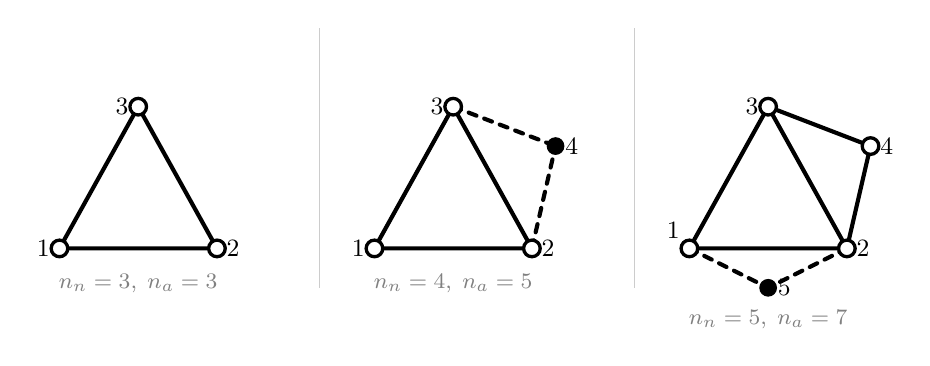
\begin{tikzpicture}[
			scale=1.0,
			asta/.style={line width=1.5pt, line cap=round,
				line join=round, black},
			nuova/.style={line width=1.5pt, line cap=round,
				line join=round, black, dashed},
			nodo/.style={circle, fill=white, draw=black,
				inner sep=0pt, minimum size=6pt,
				line width=1.2pt},
			nuovonodo/.style={circle, fill=black,
				draw=black, inner sep=0pt,
				minimum size=6pt},
			]
			\draw[very thin, gray!40](3.8,-0.5)--(3.8,2.8);
			\draw[very thin, gray!40](7.8,-0.5)--(7.8,2.8);
			
			\coordinate (A0) at (0.5, 0);
			\coordinate (B0) at (2.5, 0);
			\coordinate (C0) at (1.5, 1.8);
			\draw[asta](A0)--(B0)--(C0)--(A0);
			\node[nodo] at (A0){}; \node[nodo] at (B0){};
			\node[nodo] at (C0){};
			\node[left, font=\small] at (A0){$1$};
			\node[right,font=\small] at (B0){$2$};
			\node[left, font=\small] at (C0){$3$};
			\node[font=\footnotesize,gray] at (1.5,-0.45)
			{$n_n=3,\;n_a=3$};
			
			\coordinate (A1) at (4.5, 0);
			\coordinate (B1) at (6.5, 0);
			\coordinate (C1) at (5.5, 1.8);
			\coordinate (D1) at (6.8, 1.3);
			\draw[asta](A1)--(B1)--(C1)--(A1);
			\draw[nuova](B1)--(D1);
			\draw[nuova](C1)--(D1);
			\node[nodo] at (A1){}; \node[nodo] at (B1){};
			\node[nodo] at (C1){}; \node[nuovonodo] at (D1){};
			\node[left, font=\small] at (A1){$1$};
			\node[right,font=\small] at (B1){$2$};
			\node[left, font=\small] at (C1){$3$};
			\node[right,font=\small] at (D1){$4$};
			\node[font=\footnotesize,gray] at (5.5,-0.45)
			{$n_n=4,\;n_a=5$};
			
			\coordinate (A2) at (8.5,  0);
			\coordinate (B2) at (10.5, 0);
			\coordinate (C2) at (9.5,  1.8);
			\coordinate (D2) at (10.8, 1.3);
			\coordinate (E2) at (9.5, -0.5);
			\draw[asta](A2)--(B2)--(C2)--(A2);
			\draw[asta](B2)--(D2);
			\draw[asta](C2)--(D2);
			\draw[nuova](A2)--(E2);
			\draw[nuova](B2)--(E2);
			\node[nodo] at (A2){}; \node[nodo] at (B2){};
			\node[nodo] at (C2){}; \node[nodo] at (D2){};
			\node[nuovonodo] at (E2){};
			\node[above left,font=\small] at (A2){$1$};
			\node[right,     font=\small] at (B2){$2$};
			\node[left,      font=\small] at (C2){$3$};
			\node[right,     font=\small] at (D2){$4$};
			\node[right,     font=\small] at (E2){$5$};
			\node[font=\footnotesize,gray] at (9.5,-0.90)
			{$n_n=5,\;n_a=7$};
		\end{tikzpicture}
		\caption{Costruzione gerarchica di una travatura
			reticolare internamente isostatica.
			A sinistra: triangolo base ($n_n = 3$,
			$n_a = 3$). Al centro: aggiunta del primo
			nodo ($n_n = 4$, $n_a = 5$). A destra:
			aggiunta del secondo nodo ($n_n = 5$,
			$n_a = 7$). In ciascun passo le due aste
			nuove sono tratteggiate e il nuovo nodo è
			indicato con un cerchio pieno.}
		\label{fig:reticolare_gerarchia}
	\end{figure}
	%%%%%%%%%%%%%%%%%%%%%%%%%%%%%%%%%%%%%%%%%%%
\end{oss}


La formula di M\"{u}ller-Breslau~\EQUref{eq:muller_breslau}
conteggia in un unico indice $\nu$ il contributo di
due fonti distinte di vincolo: i vincoli esterni
(i $m_\text{est}$ gradi di libertà sottratti dai
dispositivi di appoggio al suolo) e i vincoli interni
(le $n_a$ equazioni di inestensibilità imposte dalle
aste). Quando $\nu < 0$, il sistema è
cinematicamente sovradeterminato di grado $g = -\nu$,
ma la natura fisica della sovradeterminazione dipende
da quale delle due fonti risulta in eccesso.
È quindi utile separare il contributo esterno da
quello interno e analizzarli indipendentemente.


%............................................................................................................................
\subsection{Sovradeterminazione esterna}
\label{subsec:sovradet_est}
%............................................................................................................................

Si parla di \emph{sovradeterminazione esterna}\index{sovradeterminazione!esterna} quando
il numero di componenti di reazione vincolare
$m_\text{est}$ eccede il minimo di tre necessario
per impedire i moti rigidi d'insieme nel piano.
Il grado di sovradeterminazione esterna è
\begin{equation}\label{eq:g_est}
	g_\text{est} = m_\text{est} - 3,
\end{equation}
purché i vincoli esterni siano geometricamente
indipendenti (condizione analoga a quella già
discussa per i sistemi di corpi rigidi nel
\CAPref{cap:classificazione_SCR}).

La sovradeterminazione esterna ha una conseguenza
cinematica precisa: i cedimenti dei vincoli al suolo
non sono cinematicamente liberi, ma devono soddisfare
$g_\text{est}$ condizioni di compatibilità. In assenza
di deformabilità delle aste, un cedimento non
compatibile è semplicemente impossibile: la travatura
si comporta come un \emph{corpo rigido reticolare}
i cui vincoli al suolo devono essere mutuamente
consistenti.

La sovradeterminazione esterna influenza le reazioni
vincolari, che non sono univocamente determinate
dall'equilibrio globale, ma non altera la
distribuzione degli sforzi interni nelle aste
per i sistemi esternamente iperstatici ma
internamente isostatici.


%............................................................................................................................
\subsection{Sovradeterminazione interna}
\label{subsec:sovradet_int}
%............................................................................................................................

Si parla di \emph{sovradeterminazione interna}\index{sovradeterminazione!interna} quando
il numero di aste $n_a$ eccede il valore $2n_n - 3$
richiesto dalla condizione di isostaticità interna
(con $m_\text{est} = 3$). Il grado di
sovradeterminazione interna è
\begin{equation}\label{eq:g_int}
	g_\text{int} = n_a - (2n_n - 3).
\end{equation}
Le $g_\text{int}$ aste in eccesso sono dette
\emph{aste ridondanti}\index{asta!ridondante|textbf}: la loro presenza non è
necessaria per l'equilibrio della struttura
isostatica equivalente, ma ne modifica la
distribuzione degli sforzi interni.

La sovradeterminazione interna ha una conseguenza
cinematica duale: le distorsioni estensionali delle
aste devono soddisfare $g_\text{int}$ condizioni di
compatibilità interna, ossia le distorsioni non
possono essere assegnate liberamente asta per asta
senza violare la congruenza globale della travatura.
La determinazione degli sforzi nelle aste ridondanti
richiede pertanto le relazioni costitutive e le
condizioni di congruenza del problema elastico,
che sono sviluppate nel Vol.~II.


%............................................................................................................................
\subsection{Grado di sovradeterminazione totale}
\label{subsec:sovradet_tot}
%............................................................................................................................

Il grado di sovradeterminazione totale si ottiene
sommando i due contributi:
\begin{equation}\label{eq:g_tot}
	g = g_\text{est} + g_\text{int}
	= (m_\text{est} - 3) + \bigl(n_a - (2n_n - 3)\bigr)
	= n_a + m_\text{est} - 2n_n,
\end{equation}
che è esattamente $-\nu$ dalla
formula~\EQUref{eq:muller_breslau}. Il
conteggio globale non distingue le due fonti, ma la
loro separazione è indispensabile per impostare
correttamente l'analisi.

\begin{oss}
	Una travatura può essere esternamente isostatica
	e internamente iperstatica ($g_\text{est} = 0$,
	$g_\text{int} > 0$): i vincoli al suolo sono
	minimi e le reazioni si determinano dall'equilibrio
	globale, ma la distribuzione degli sforzi nelle aste
	è indeterminata. Viceversa, può essere esternamente
	iperstatica e internamente isostatica ($g_\text{est} > 0$,
	$g_\text{int} = 0$): gli sforzi nelle aste di ogni
	troncone isostatico si determinano dall'equilibrio,
	ma le reazioni al suolo non sono univocamente
	determinate dal solo equilibrio globale.
	I due gradi di sovradeterminazione hanno quindi
	conseguenze fisiche e operative distinte e
	non si sostituiscono a vicenda.
\end{oss}



%----------------------------------------------------------------------------------------------------------------------------
\section{Morfologia delle travature reticolari}
\label{sec:morfologia_reticolari}
%----------------------------------------------------------------------------------------------------------------------------

Prima di sviluppare i metodi di analisi, è utile
disporre di un quadro morfologico delle travature
reticolari: le parti che le compongono, le famiglie
geometriche più comuni, i sistemi complessi formati
da più travature collegate, e i principali schemi
tridimensionali. Questo catalogo ha un duplice scopo:
fornire la terminologia di riferimento che sarà usata
in tutto il capitolo --- in particolare nelle sezioni
dedicate al metodo di Ritter e all'analogia della trave
equivalente --- e mostrare concretamente la varietà
delle strutture che la teoria sviluppata è in grado
di trattare.


%............................................................................................................................
\subsection{Parti della travatura reticolare piana}
\label{subsec:parti_travatura}
%............................................................................................................................

Nelle travature reticolari piane a sviluppo
prevalentemente orizzontale si distinguono
convenzionalmente tre gruppi di aste
(si veda la \FIGref{fig:parti_travatura}):

\begin{itemize}
	\item le \emph{aste del corrente superiore}\index{corrente|textbf}\index{corrente!superiore|textbf},
	dette anche \emph{aste di estradosso}\index{estradosso},
	che formano il bordo superiore della
	travatura e assorbono prevalentemente
	sforzi di compressione sotto carichi
	verticali discendenti;
	
	\item le \emph{aste del corrente inferiore}\index{corrente!inferiore|textbf},
	dette anche \emph{aste di intradosso}\index{intradosso},
	che formano il bordo inferiore e lavorano
	prevalentemente a trazione, svolgendo la
	funzione di \emph{catena};
	
	\item le \emph{aste di parete}\index{asta!di parete|textbf}, suddivise in
	\emph{montanti}\index{montante|textbf} --- aste verticali o
	comunque trasversali all'asse della
	travatura --- e \emph{diagonali}\index{diagonale|textbf} --- aste
	inclinate rispetto all'asse.
\end{itemize}


%%%%%%%%%%%%%%%%%%%%%%%%%%%%%%%%%%%%%%%%%%%
\begin{figure}[htbp]
	\centering
	\resizebox{\textwidth}{!}{%
		\begin{tikzpicture}[
			asta/.style={line width=1.5pt, line cap=round, line join=round, black},
			cord/.style={line width=1.5pt, line cap=round, line join=round, black},
			nodo/.style={circle, fill=white, draw=black,
				inner sep=0pt, minimum size=5pt, line width=1.0pt},
			terra/.style={line width=0.7pt, black},
			richiamo/.style={->, >=stealth, line width=0.6pt, black},
			]
			\def\d{1.0}
			\def\h{0.95}
			
			%% =========================================================
			%% (a) TRAVATURA A CORRENTI PARALLELI (mensola con tirante)
			%% =========================================================
			\begin{scope}[xshift=0cm]
				
				%% ── Correnti ─────────────────────────────────────────
				\draw[cord](0,0)--(7*\d,0);
				\draw[cord](\d,\h)--(8*\d,\h);
				
				%% ── Montanti ─────────────────────────────────────────
				\foreach \i in {1,...,7}
				\draw[asta](\i*\d,0)--(\i*\d,\h);
				
				%% ── Diagonali ────────────────────────────────────────
				\foreach \i in {0,...,7}
				\draw[asta](\i*\d,0)--(\i*\d+\d,\h);
				
				%% ── Tirante a parete ─────────────────────────────────
				\coordinate (W) at (-0.9, 2.5);
				\draw[asta](W)--(3*\d,\h);
				%% cerniera a base verticale
				\draw[line width=1.0pt](W)--++(-0.40,-0.24)--++(0,0.48)--cycle;
				\draw[line width=1.0pt]($(W)+(-0.40,-0.34)$)--($(W)+(-0.40,0.34)$);
				\foreach \yy in {-0.28,-0.14,0.00,0.14,0.28}
				\draw[very thin]($(W)+(-0.40,\yy)$)--++(-0.13,-0.10);
				
				%% ── Cerniera a terra nel nodo di sinistra ────────────
				\draw[line width=1.0pt](0,0)--++(-0.24,-0.40)--++(0.48,0)--cycle;
				\draw[line width=1.0pt](-0.34,-0.40)--(0.34,-0.40);
				\foreach \x in {-0.28,-0.14,0.00,0.14,0.28}
				\draw[very thin](\x,-0.40)--++(-.10,-0.13);
				
				%% ── Nodi ─────────────────────────────────────────────
				\node[nodo]at(W){};
				\foreach \i in {0,...,7} \node[nodo]at(\i*\d,0){};
				\foreach \i in {1,...,8} \node[nodo]at(\i*\d,\h){};
				
				%% ── Etichette con richiami ───────────────────────────
				\draw[richiamo](3.6,1.85)--(4.5*\d,\h+0.04);
				\node[right,font=\small]at(3.6,1.85){corrente superiore};
				
				\draw[richiamo](5.8,-0.75)--(5.5*\d,-0.05);
				\node[right,font=\small]at(5.8,-0.75){corrente inferiore};
				
				\draw[richiamo](1.3,-0.85)--(2*\d-0.04,0.5*\h);
				\node[left,font=\small]at(1.3,-0.85){montante};
				
				\draw[richiamo](2.9,-0.85)--(3.5*\d-0.06,0.40*\h);
				\node[right,font=\small]at(2.9,-0.85){asta diagonale};
				
				\node[font=\small]at(1.5,-1.45){(a)};
			\end{scope}
			
			%% =========================================================
			%% (b) TRAVATURA AD ARCO (correnti curvi)
			%% =========================================================
			\begin{scope}[xshift=10.5cm, yshift=-0.cm]
				
				%% ── Correnti curvi (archi di cerchio) ────────────────
				%% intradosso interrotto alla chiave: archi A->I2 e I3->B
				%% (R=5.212, centro (3.5,-3.862))
				\draw[cord] (0,0) arc[start angle=132.18, end angle=97.03, radius=5.212];
				\draw[cord] (4.138,1.311) arc[start angle=82.97, end angle=47.82, radius=5.212];
				%% estradosso: R=3.967, centro (3.5,-1.867), 151.93° -> 28.07°
				\draw[cord] (0,0) arc[start angle=151.93, end angle=28.07, radius=3.967];
				
				%% ── Nodi (coordinate precalcolate) ───────────────────
				\coordinate (A)  at (0,0);
				\coordinate (B)  at (7,0);
				\coordinate (E1) at (0.883,1.114);
				\coordinate (E2) at (2.102,1.845);
				\coordinate (C)  at (3.500,2.100);
				\coordinate (E4) at (4.898,1.845);
				\coordinate (E5) at (6.117,1.114);
				\coordinate (I1) at (1.624,1.001);
				\coordinate (I2) at (2.862,1.311);
				\coordinate (I3) at (4.138,1.311);
				\coordinate (I4) at (5.376,1.001);
				
				%% ── Aste di parete (zig-zag) ─────────────────────────
				\draw[asta](E1)--(I1)--(E2)--(I2)--(C)--(I3)--(E4)--(I4)--(E5);
				
				%% ── Cerniera in A ────────────────────────────────────
				\draw[line width=1.0pt](A)--++(-0.24,-0.40)--++(0.48,0)--cycle;
				\draw[line width=1.0pt](-0.34,-0.40)--(0.34,-0.40);
				\foreach \x in {-0.28,-0.14,0.00,0.14,0.28}
				\draw[very thin](\x,-0.40)--++(-.10,-0.13);
				
				%% ── Cerniera in B ────────────────────────────────────
				\draw[line width=1.0pt](B)--++(-0.24,-0.40)--++(0.48,0)--cycle;
				\draw[line width=1.0pt]($(B)+(-0.34,-0.40)$)--($(B)+(0.34,-0.40)$);
				\foreach \x in {-0.28,-0.14,0.00,0.14,0.28}
				\draw[very thin]($(B)+(\x,-0.40)$)--++(-.10,-0.13);
				
				%% ── Nodi ─────────────────────────────────────────────
				\foreach \n in {A,B,E1,E2,C,E4,E5,I1,I2,I3,I4}
				\node[nodo]at(\n){};
				
				%% ── Etichette nodi ───────────────────────────────────
				\node[left, font=\small]at($(A)+(-0.12,0.10)$){$A$};
				\node[right,font=\small]at($(B)+( 0.12,0.10)$){$B$};
				\node[above,font=\small]at($(C)+(0,0.10)$){$C$};
				
				%% ── Etichette con richiami ───────────────────────────
				\draw[richiamo](5.3,2.65)--($(E4)!0.5!(E5)+(0.13,0.13)$);
				\node[right,font=\small]at(5.3,2.65){corrente di estradosso};
				
				\draw[richiamo](3.2,0.62)--($(I1)!0.45!(E2)$);
				\draw[richiamo](3.8,0.62)--($(I3)!0.55!(E4)$);
				\node[font=\small, align=center]at(3.5,0.28){aste di\\parete};
				
				\draw[richiamo](4.6,-1.15)--($(A)!0.30!(I1)+(0.10,-0.10)$);
				\draw[richiamo](4.6,-1.15)--($(I4)!0.55!(B)+(0.06,-0.12)$);
				\node[right,font=\small]at(4.6,-1.15){corrente di intradosso};
				
				\node[font=\small]at(1.5,-1.45){(b)};
			\end{scope}
	\end{tikzpicture}}
	\caption{Parti della travatura reticolare piana.
		(a): travatura a correnti paralleli
		(mensola con tirante ancorato a parete); si
		distinguono il corrente superiore (o di
		estradosso), il corrente inferiore (o di
		intradosso) e le aste di parete, suddivise
		in montanti e diagonali.
		(b): arco reticolare a tre cerniere
		($A$, $C$, $B$) a correnti curvi; le stesse
		denominazioni si applicano con riferimento al
		corrente di estradosso e al corrente di
		intradosso, entrambi curvilinei, raccordati
		dalle aste di parete; il corrente di intradosso
		è interrotto alla chiave, dove il nodo $C$
		funge da cerniera tra i due semiarchi.}
	\label{fig:parti_travatura}
\end{figure}
%%%%%%%%%%%%%%%%%%%%%%%%%%%%%%%%%%%%%%%%%%%



\begin{oss}
	La terminologia \emph{estradosso/intradosso}
	è mutuata dall'architettura degli archi, dove
	indica rispettivamente il bordo esterno e
	quello interno della volta. Nelle travature
	orizzontali con carichi verticali discendenti,
	l'intradosso coincide con il corrente inferiore
	teso e l'estradosso con il corrente superiore
	compresso.
\end{oss}


%............................................................................................................................
\subsection{Tipologie di maglie piane}
\label{subsec:tipologie_maglie}
%............................................................................................................................

Le travature reticolari piane isostatiche più comuni
si classificano in base alla geometria delle maglie
elementari. Le famiglie principali sono illustrate
nella \FIGref{fig:tipologie_maglie}.


%%%%%%%%%%%%%%%%%%%%%%%%%%%%%%%%%%%%%%%%%%%
\begin{figure}[!htbp]
	\centering
	\resizebox{0.9\textwidth}{!}{%
		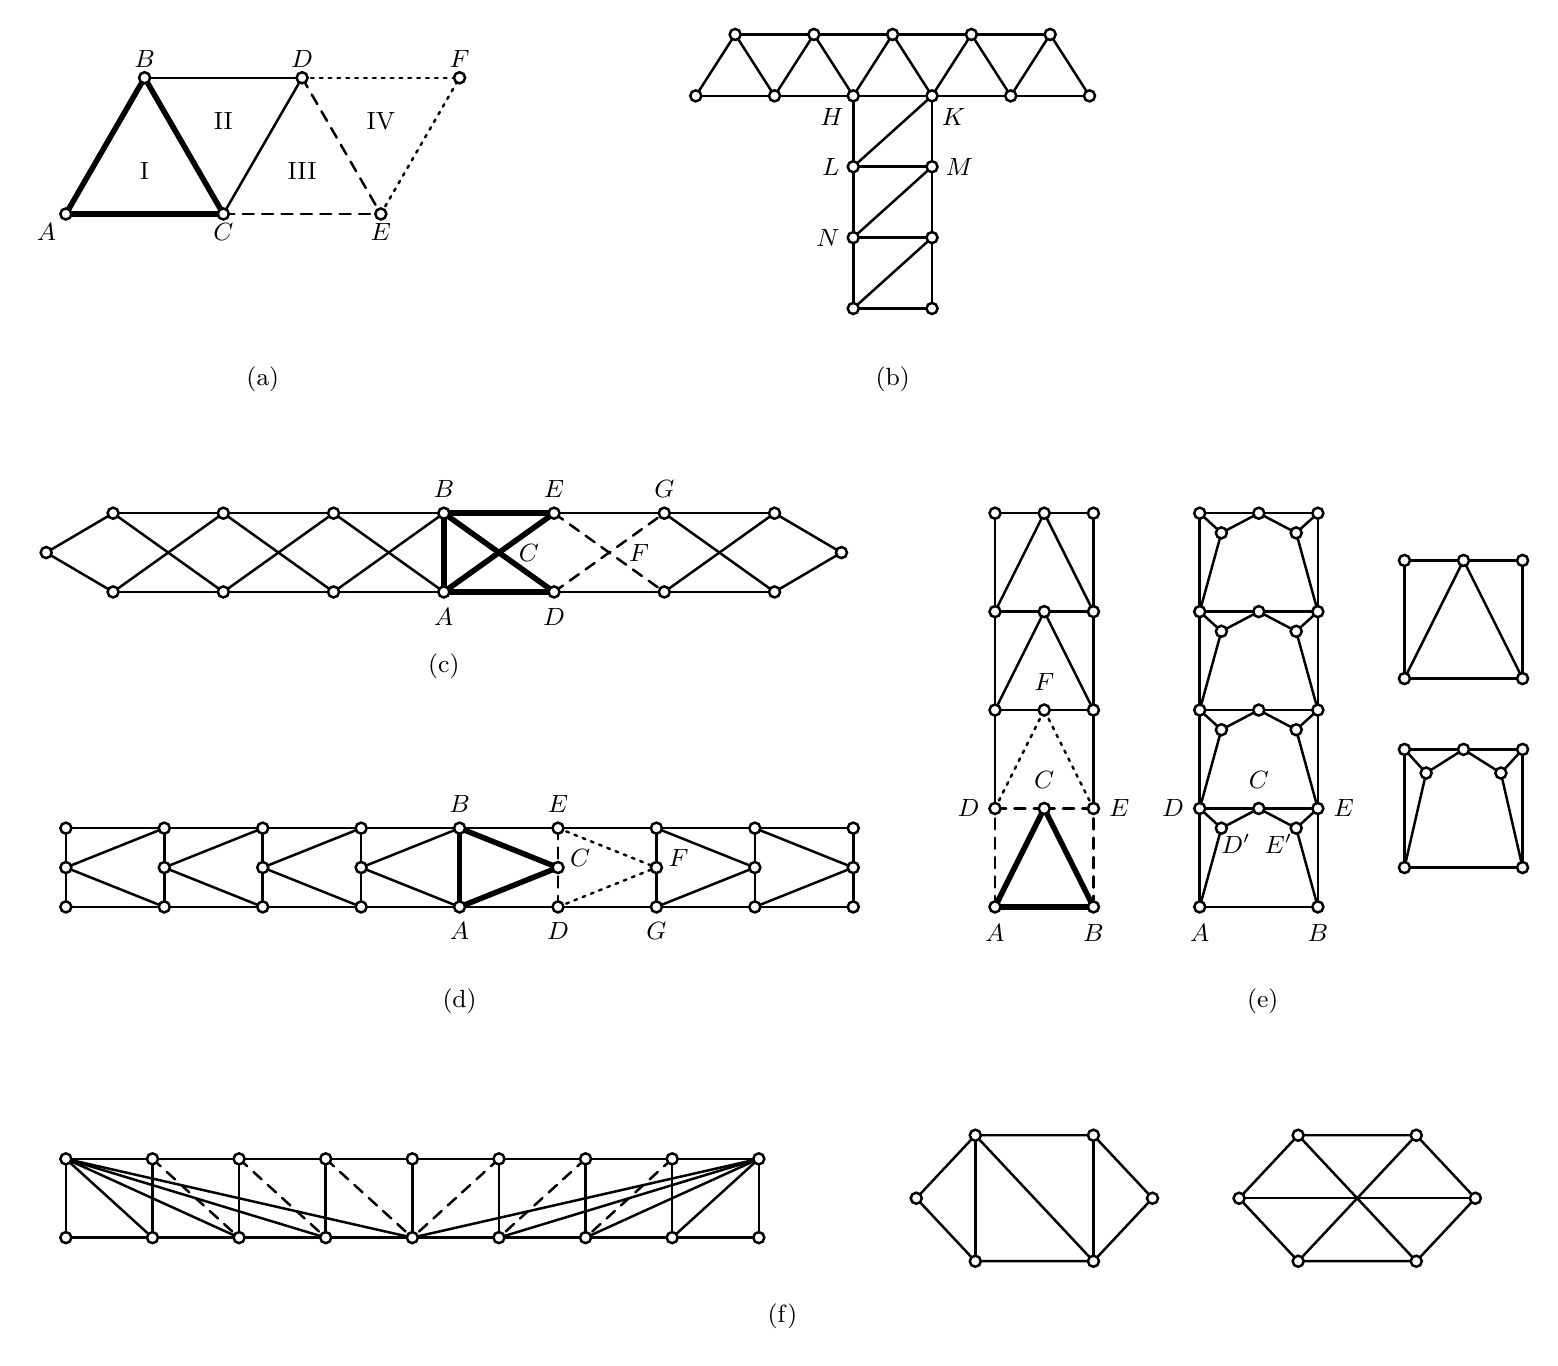
\begin{tikzpicture}[
			asta/.style={line width=0.9pt, line cap=round, line join=round, black},
			base/.style={line width=2.0pt, line cap=round, line join=round, black},
			nuova/.style={line width=0.9pt, line cap=round, line join=round, black,
				dash pattern=on 4pt off 3pt},
			futura/.style={line width=0.9pt, line cap=round, black,
				dash pattern=on 1pt off 2.2pt},
			nodo/.style={circle, fill=white, draw=black,
				inner sep=0pt, minimum size=4.0pt, line width=0.9pt},
			etich/.style={font=\small},
			pan/.style={font=\small},
			]
			
			%% =========================================================
			%% (a) COMPOSIZIONE GERARCHICA A MAGLIE TRIANGOLARI
			%% =========================================================
			\begin{scope}[xshift=0cm, yshift=-1.0cm]
				\coordinate (aA) at (0,0);
				\coordinate (aC) at (2,0);
				\coordinate (aB) at (1,1.73);
				\coordinate (aD) at (3,1.73);
				\coordinate (aE) at (4,0);
				\coordinate (aF) at (5,1.73);
				%% maglia I (base)
				\draw[base](aA)--(aC)--(aB)--cycle;
				%% maglia II
				\draw[asta](aB)--(aD);
				\draw[asta](aC)--(aD);
				%% maglia III
				\draw[nuova](aC)--(aE);
				\draw[nuova](aD)--(aE);
				%% maglia IV
				\draw[futura](aD)--(aF);
				\draw[futura](aE)--(aF);
				\foreach \n in {aA,aB,aC,aD,aE,aF} \node[nodo]at(\n){};
				\node[etich,below left ]at(aA){$A$};
				\node[etich,above      ]at(aB){$B$};
				\node[etich,below      ]at(aC){$C$};
				\node[etich,above      ]at(aD){$D$};
				\node[etich,below      ]at(aE){$E$};
				\node[etich,above      ]at(aF){$F$};
				\node[etich]at(1.00,0.55){I};
				\node[etich]at(2.00,1.18){II};
				\node[etich]at(3.00,0.55){III};
				\node[etich]at(4.00,1.18){IV};
				\node[pan]at(2.5,-2.10){(a)};
			\end{scope}
			
			%% =========================================================
			%% (b) TRAVATURA RAMIFICATA
			%% =========================================================
			\begin{scope}[xshift=8.0cm, yshift=0.5cm]
				%% travatura orizzontale (Warren)
				\draw[asta](0,0)--(5,0);
				\draw[asta](0.5,0.78)--(4.5,0.78);
				\foreach \i in {0,...,4}{
					\draw[asta](\i,0)--(\i+0.5,0.78);
					\draw[asta](\i+0.5,0.78)--(\i+1,0);}
				%% ramo verticale dall'asta HK
				\draw[asta](2,0)--(2,-2.7);
				\draw[asta](3,0)--(3,-2.7);
				\draw[asta](2,-0.9)--(3,-0.9);
				\draw[asta](2,-1.8)--(3,-1.8);
				\draw[asta](2,-2.7)--(3,-2.7);
				\draw[asta](2,-0.9)--(3,0);
				\draw[asta](2,-1.8)--(3,-0.9);
				\draw[asta](2,-2.7)--(3,-1.8);
				%% nodi
				\foreach \i in {0,...,5} \node[nodo]at(\i,0){};
				\foreach \i in {0,...,4} \node[nodo]at(\i+0.5,0.78){};
				\foreach \y in {-0.9,-1.8,-2.7}{
					\node[nodo]at(2,\y){}; \node[nodo]at(3,\y){};}
				%% etichette
				\node[etich,below left ]at(2,-0.04){$H$};
				\node[etich,below right]at(3,-0.04){$K$};
				\node[etich,left ]at(1.95,-0.9){$L$};
				\node[etich,right]at(3.05,-0.9){$M$};
				\node[etich,left ]at(1.95,-1.8){$N$};
				\node[pan]at(2.5,-3.60){(b)};
			\end{scope}
			
			%% =========================================================
			%% (c) MAGLIE ROMBOIDALI
			%% =========================================================
			\begin{scope}[xshift=0.6cm, yshift=-5.8cm]
				\def\dc{1.4}
				%% correnti
				\draw[asta](0,0)--(6*\dc,0);
				\draw[asta](0,1)--(6*\dc,1);
				%% estremita' a punta
				\draw[asta](-0.85,0.5)--(0,1);
				\draw[asta](-0.85,0.5)--(0,0);
				\draw[asta](6*\dc+0.85,0.5)--(6*\dc,1);
				\draw[asta](6*\dc+0.85,0.5)--(6*\dc,0);
				%% diagonali incrociate (campate non in evidenza)
				\foreach \i in {0,1,2,5}{
					\draw[asta](\i*\dc,0)--(\i*\dc+\dc,1);
					\draw[asta](\i*\dc,1)--(\i*\dc+\dc,0);}
				%% maglia generatrice in evidenza: montante AB + campata ABED
				\draw[base](3*\dc,0)--(3*\dc,1);
				\draw[base](3*\dc,0)--(4*\dc,0);
				\draw[base](3*\dc,1)--(4*\dc,1);
				\draw[base](3*\dc,0)--(4*\dc,1);
				\draw[base](3*\dc,1)--(4*\dc,0);
				%% passo successivo: diagonali D-G ed E-H (tratteggiate)
				\draw[nuova](4*\dc,0)--(5*\dc,1);
				\draw[nuova](4*\dc,1)--(5*\dc,0);
				%% passo ancora successivo: correnti E-G e D-H (punteggiati)
				\draw[futura](4*\dc,1)--(5*\dc,1);
				\draw[futura](4*\dc,0)--(5*\dc,0);
				%% nodi
				\foreach \i in {0,...,6}{
					\node[nodo]at(\i*\dc,0){}; \node[nodo]at(\i*\dc,1){};}
				\node[nodo]at(-0.85,0.5){};
				\node[nodo]at(6*\dc+0.85,0.5){};
				%% etichette (C ed F: incroci senza nodo strutturale)
				\node[etich,below]at(3*\dc,-0.08){$A$};
				\node[etich,above]at(3*\dc, 1.08){$B$};
				\node[etich]at(3.5*\dc+0.38,0.50){$C$};
				\node[etich,below]at(4*\dc,-0.08){$D$};
				\node[etich,above]at(4*\dc, 1.08){$E$};
				\node[etich]at(4.5*\dc+0.38,0.50){$F$};
				\node[etich,above]at(5*\dc, 1.08){$G$};
				\node[pan]at(3*\dc,-0.95){(c)};
			\end{scope}
			
			%% =========================================================
			%% (d.1) MAGLIE A K --- travatura orizzontale
			%% =========================================================
			\begin{scope}[xshift=0cm, yshift=-9.8cm]
				\def\dk{1.25}
				%% correnti
				\draw[asta](0,0)--(8*\dk,0);
				\draw[asta](0,1)--(8*\dk,1);
				%% montanti
				\foreach \i in {0,1,2,3,4,6,7,8}
				\draw[asta](\i*\dk,0)--(\i*\dk,1);
				%% diagonali a K: meta' sinistra convergenti a sinistra
				\foreach \i in {0,1,2,3}{
					\draw[asta]({(\i+1)*\dk},0)--(\i*\dk,0.5);
					\draw[asta]({(\i+1)*\dk},1)--(\i*\dk,0.5);}
				%% meta' destra: campate gia' composte
				\foreach \i in {6,7}{
					\draw[asta](\i*\dk,0)--({(\i+1)*\dk},0.5);
					\draw[asta](\i*\dk,1)--({(\i+1)*\dk},0.5);}
				%% generazione in evidenza: triangolo A-B-C
				\draw[base](4*\dk,0)--(4*\dk,1);
				\draw[base](4*\dk,0)--(5*\dk,0.5);
				\draw[base](4*\dk,1)--(5*\dk,0.5);
				%% passo successivo: nodi D, E (correnti + mezzi montanti)
				\draw[nuova](4*\dk,0)--(5*\dk,0);
				\draw[nuova](4*\dk,1)--(5*\dk,1);
				\draw[nuova](5*\dk,0)--(5*\dk,0.5);
				\draw[nuova](5*\dk,1)--(5*\dk,0.5);
				%% passo ancora successivo: nodi F, G
				\draw[futura](5*\dk,0)--(6*\dk,0.5);
				\draw[futura](5*\dk,1)--(6*\dk,0.5);
				\draw[futura](5*\dk,0)--(6*\dk,0);
				\draw[futura](6*\dk,0)--(6*\dk,0.5);
				%% nodi
				\foreach \i in {0,...,8}{
					\node[nodo]at(\i*\dk,0){}; \node[nodo]at(\i*\dk,1){};}
				\foreach \i in {0,1,2,3,5,6,7,8} \node[nodo]at(\i*\dk,0.5){};
				%% etichette
				\node[etich,below]at(4*\dk,-0.08){$A$};
				\node[etich,above]at(4*\dk, 1.08){$B$};
				\node[etich]at(5*\dk+0.28,0.62){$C$};
				\node[etich,below]at(5*\dk,-0.08){$D$};
				\node[etich,above]at(5*\dk, 1.08){$E$};
				\node[etich]at(6*\dk+0.28,0.62){$F$};
				\node[etich,below]at(6*\dk,-0.08){$G$};
			\end{scope}
			
			%% =========================================================
			%% (e.1) TORRI A K --- variante con nodo sul traverso
			%% =========================================================
			\begin{scope}[xshift=11.8cm, yshift=-9.8cm, scale=1.25]
				%% concio generativo
				\draw[base](0,0)--(1,0);
				\draw[base](0,0)--(0.5,1);
				\draw[base](1,0)--(0.5,1);
				\draw[nuova](0,0)--(0,1);
				\draw[nuova](1,0)--(1,1);
				\draw[nuova](0,1)--(0.5,1);
				\draw[nuova](1,1)--(0.5,1);
				\draw[futura](0,1)--(0.5,2);
				\draw[futura](1,1)--(0.5,2);
				%% conci superiori
				\draw[asta](0,1)--(0,4);
				\draw[asta](1,1)--(1,4);
				\draw[asta](0,2)--(1,2);
				\draw[asta](0,3)--(1,3);
				\draw[asta](0,4)--(1,4);
				\draw[asta](0,2)--(0.5,3);
				\draw[asta](1,2)--(0.5,3);
				\draw[asta](0,3)--(0.5,4);
				\draw[asta](1,3)--(0.5,4);
				%% nodi
				\foreach \y in {0,...,4}{
					\node[nodo]at(0,\y){}; \node[nodo]at(1,\y){};}
				\foreach \y in {1,...,4} \node[nodo]at(0.5,\y){};
				%% etichette
				\node[etich,below]at(0,-0.08){$A$};
				\node[etich,below]at(1,-0.08){$B$};
				\node[etich,left ]at(-0.06,1){$D$};
				\node[etich,right]at(1.06,1){$E$};
				\node[etich,above]at(0.5,1.10){$C$};
				\node[etich,above]at(0.5,2.10){$F$};
			\end{scope}
			
			%% =========================================================
			%% (e.2) TORRI A K --- variante a diagonali simmetriche
			%% =========================================================
			\begin{scope}[xshift=14.4cm, yshift=-9.8cm, scale=1.25]
				\foreach \k in {0,...,3}{
					\begin{scope}[yshift=\k cm]
						\draw[asta](0,0)--(0,1);
						\draw[asta](1.2,0)--(1.2,1);
						\draw[asta](0,1)--(0.6,1);
						\draw[asta](0.6,1)--(1.2,1);
						\draw[asta](0,0)--(0.22,0.80);
						\draw[asta](0.22,0.80)--(0,1);
						\draw[asta](0.22,0.80)--(0.6,1);
						\draw[asta](1.2,0)--(0.98,0.80);
						\draw[asta](0.98,0.80)--(1.2,1);
						\draw[asta](0.98,0.80)--(0.6,1);
				\end{scope}}
				\draw[asta](0,0)--(1.2,0);
				%% nodi
				\foreach \y in {0,...,4}{
					\node[nodo]at(0,\y){}; \node[nodo]at(1.2,\y){};}
				\foreach \y in {1,...,4} \node[nodo]at(0.6,\y){};
				\foreach \k in {0,...,3}{
					\node[nodo]at(0.22,{\k+0.80}){};
					\node[nodo]at(0.98,{\k+0.80}){};}
				%% etichette
				\node[etich,below]at(0,-0.08){$A$};
				\node[etich,below]at(1.2,-0.08){$B$};
				\node[etich,left ]at(-0.06,1){$D$};
				\node[etich,right]at(1.26,1){$E$};
				\node[etich,above]at(0.6,1.10){$C$};
				\node[etich,right]at(0.12,0.64){$D'$};
				\node[etich,below]at(0.80,0.84){$E'$};
			\end{scope}
			
			%% =========================================================
			%% (e.3) maglie elementari delle due varianti
			%% =========================================================
			\begin{scope}[xshift=17.0cm, yshift=-6.9cm, scale=1.25]
				%% maglia con nodo sul traverso
				\draw[asta](0,0)--(1.2,0)--(1.2,1.2)--(0,1.2)--cycle;
				\draw[asta](0,0)--(0.6,1.2);
				\draw[asta](1.2,0)--(0.6,1.2);
				\foreach \p in {(0,0),(1.2,0),(0,1.2),(0.6,1.2),(1.2,1.2)}
				\node[nodo]at\p{};
			\end{scope}
			\begin{scope}[xshift=17.0cm, yshift=-9.3cm, scale=1.25]
				%% maglia a diagonali simmetriche
				\draw[asta](0,0)--(1.2,0)--(1.2,1.2)--(0,1.2)--cycle;
				\draw[asta](0,0)--(0.22,0.96);
				\draw[asta](0.22,0.96)--(0,1.2);
				\draw[asta](0.22,0.96)--(0.6,1.2);
				\draw[asta](1.2,0)--(0.98,0.96);
				\draw[asta](0.98,0.96)--(1.2,1.2);
				\draw[asta](0.98,0.96)--(0.6,1.2);
				\foreach \p in {(0,0),(1.2,0),(0,1.2),(0.6,1.2),(1.2,1.2),
					(0.22,0.96),(0.98,0.96)}
				\node[nodo]at\p{};
			\end{scope}
			
			\node[pan]at(5.0,-11.0){(d)};
			
			\node[pan]at(15.2,-11.0){(e)};
			
			%% =========================================================
			%% (f.1) SCHEMA IBRIDO: diagonali a ventaglio
			%% =========================================================
			\begin{scope}[xshift=0cm, yshift=-14.0cm]
				\def\de{1.1}
				\draw[asta](0,0)--(8*\de,0);
				\draw[asta](0,1)--(8*\de,1);
				\foreach \i in {0,...,8} \draw[asta](\i*\de,0)--(\i*\de,1);
				%% ventaglio dalle estremita' superiori
				\foreach \j in {1,2,3,4} \draw[asta](0,1)--(\j*\de,0);
				\foreach \j in {7,6,5,4} \draw[asta](8*\de,1)--(\j*\de,0);
				%% aste sostituite (tratteggiate)
				\foreach \i in {1,2,3} \draw[nuova](\i*\de,1)--({(\i+1)*\de},0);
				\foreach \i in {7,6,5} \draw[nuova](\i*\de,1)--({(\i-1)*\de},0);
				\foreach \i in {0,...,8}{
					\node[nodo]at(\i*\de,0){}; \node[nodo]at(\i*\de,1){};}
			\end{scope}
			
			%% =========================================================
			%% (f.2) SCHEMI IBRIDI ESAGONALI
			%% =========================================================
			\begin{scope}[xshift=10.8cm, yshift=-14.3cm]
				\coordinate (hL)  at (0,0.8);
				\coordinate (htl) at (0.75,1.6);
				\coordinate (htr) at (2.25,1.6);
				\coordinate (hR)  at (3,0.8);
				\coordinate (hbr) at (2.25,0);
				\coordinate (hbl) at (0.75,0);
				\draw[asta](hL)--(htl)--(htr)--(hR)--(hbr)--(hbl)--cycle;
				\draw[asta](htl)--(hbl);
				\draw[asta](htl)--(hbr);
				\draw[asta](htr)--(hbr);
				\foreach \n in {hL,htl,htr,hR,hbr,hbl} \node[nodo]at(\n){};
			\end{scope}
			\begin{scope}[xshift=14.9cm, yshift=-14.3cm]
				\coordinate (kL)  at (0,0.8);
				\coordinate (ktl) at (0.75,1.6);
				\coordinate (ktr) at (2.25,1.6);
				\coordinate (kR)  at (3,0.8);
				\coordinate (kbr) at (2.25,0);
				\coordinate (kbl) at (0.75,0);
				\draw[asta](kL)--(ktl)--(ktr)--(kR)--(kbr)--(kbl)--cycle;
				\draw[asta](kL)--(kR);
				\draw[asta](ktl)--(kbr);
				\draw[asta](ktr)--(kbl);
				\foreach \n in {kL,ktl,ktr,kR,kbr,kbl} \node[nodo]at(\n){};
			\end{scope}
			
			\node[pan]at(9.1,-15.0){(f)};
			
	\end{tikzpicture}}
	\caption{Tipologie di maglie nelle travature reticolari
		piane isostatiche.
		(a): composizione gerarchica a maglie
		triangolari; i nodi sono aggiunti progressivamente
		e le aste nuove sono tratteggiate.
		(b): travatura ramificata, ottenuta
		avviando la composizione da un'asta intermedia
		anziché da un nodo.
		(c): maglie romboidali; le diagonali
		si incrociano senza nodo strutturale.
		(d): maglie a K, con i montanti spezzati
		a metà altezza dal nodo su cui convergono
		le diagonali.
		(e): varianti a torre della maglia a K,
		con nodo sul traverso e a diagonali simmetriche;
		a fianco le rispettive maglie elementari.
		(f): schemi ibridi con aste di parete
		non standard: nello schema a ventaglio le aste
		tratteggiate sono le diagonali dello schema
		triangolare di partenza, soppresse e sostituite
		dalle aste uscenti a ventaglio dai nodi estremi
		del corrente superiore.}
	\label{fig:tipologie_maglie}
\end{figure}
%%%%%%%%%%%%%%%%%%%%%%%%%%%%%%%%%%%%%%%%%%%



\esottotit{Maglie triangolari.}
Sono le più diffuse. Si generano per composizione
gerarchica a partire da un triangolo base, aggiungendo
ad ogni passo un nodo e due aste: la procedura è
discussa nel \CAPref{cap:assemblaggi_travi}
(\OSSref{oss:composizione_gerarchica}) e garantisce
l'isostaticità interna $n_a = 2n_n - 3$ ad ogni
passo. Il processo di aggiunta può avvenire anche
su un'asta intermedia anziché su un nodo esistente,
dando luogo a \emph{diramazioni}: la travatura
ramificata di \FIGref{fig:tipologie_maglie}(b) è
ottenuta in questo modo.

La famiglia a maglie triangolari comprende schemi
molto diversi tra loro, illustrati nelle
\FIGrefS{fig:correnti_paralleli}
e~\ref{fig:capriate_spezzato}.
Per i correnti paralleli, le varianti principali si
distinguono per l'orientamento delle diagonali: nel
\emph{tipo Howe}~(\FIGref{fig:correnti_paralleli}a)
le diagonali interne convergono verso l'alto al centro
--- e risultano compresse sotto carichi verticali
applicati ai nodi del corrente superiore --- mentre
i montanti lavorano a trazione;
nel \emph{tipo Pratt}~(\FIGref{fig:correnti_paralleli}b)
l'orientamento è invertito --- le diagonali interne
scendono verso il centro, lavorano a trazione e i
montanti a compressione --- il che le rende più
efficienti nell'acciaio, dove la trazione non comporta
rischio di instabilità.
Il \emph{tipo Warren}~(\FIGref{fig:correnti_paralleli}c)
elimina i montanti e affida il trasferimento del taglio
alle sole diagonali alternate, riducendo il numero di
aste a parità di pannelli.

Le capriate a corrente superiore spezzato
(\FIGref{fig:capriate_spezzato}) adottano puntoni
inclinati come corrente superiore: nel profilo a
puntoni rettilinei~(a) i nodi intermedi giacciono
sulla retta appoggio--colmo; nel profilo a schiena
d'asino~(b) il corrente superiore è genuinamente
poligonale, con i nodi intermedi al di sopra di
tale retta.
Tutti gli schemi rispettano la stessa regola di
composizione gerarchica.



\begin{figure}[!htbp]
	\centering
	\resizebox{\textwidth}{!}{%
		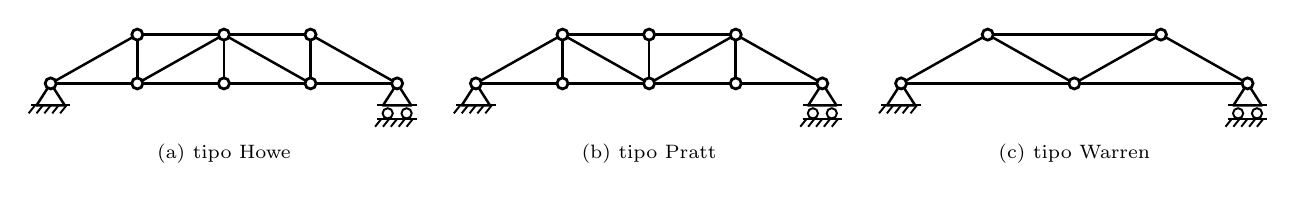
\begin{tikzpicture}[
			asta/.style={line width=0.90pt, line cap=round, line join=round, black},
			cord/.style={line width=0.90pt, line cap=round, line join=round, black},
			nodo/.style={circle, fill=white, draw=black, inner sep=0pt, minimum size=4pt, line width=1.0pt},
			terra/.style={line width=0.7pt, black},
			]
			
			
			\def\d{1.1}
			\def\h{0.62}
			
			%% ── (a) Pratt ──────────────────────────────────────────
			\begin{scope}[xshift=0cm]
				\draw[cord](0,0)--(4*\d,0);
				\draw[cord](\d,\h)--(3*\d,\h);
				\draw[asta](\d,0)--(\d,\h);
				\draw[asta](2*\d,0)--(2*\d,\h);
				\draw[asta](3*\d,0)--(3*\d,\h);
				\draw[asta](0,0)--(\d,\h);
				\draw[asta](\d,0)--(2*\d,\h);
				\draw[asta](3*\d,0)--(2*\d,\h);
				\draw[asta](4*\d,0)--(3*\d,\h);
				\draw[cord](0,0)--(-0.18,-0.28)--(0.18,-0.28)--cycle;
				\draw[terra](-0.25,-0.28)--(0.25,-0.28);
				\foreach \xx in {-0.20,-0.10,0,0.10,0.20}
				\draw[terra](\xx,-0.28)--++(-0.08,-0.10);
				\draw[cord](4*\d,0)--(4*\d-0.18,-0.28)--(4*\d+0.18,-0.28)--cycle;
				\draw[terra](4*\d-0.25,-0.28)--(4*\d+0.25,-0.28);
				\draw[terra](4*\d-0.12,-0.38)circle(0.065);
				\draw[terra](4*\d+0.12,-0.38)circle(0.065);
				\draw[terra](4*\d-0.25,-0.45)--(4*\d+0.25,-0.45);
				\foreach \xx in {-0.20,-0.10,0,0.10,0.20}
				\draw[terra](4*\d+\xx,-0.45)--++(-0.08,-0.10);
				\foreach \x in {0,1,2,3,4} \node[nodo]at(\x*\d,0){};
				\foreach \x in {1,2,3}     \node[nodo]at(\x*\d,\h){};
				\node[below,font=\scriptsize]at(2*\d,-0.65){(a) tipo Howe};
			\end{scope}
			
			%% ── (b) Howe ───────────────────────────────────────────
			\begin{scope}[xshift=5.4cm]
				\draw[cord](0,0)--(4*\d,0);
				\draw[cord](\d,\h)--(3*\d,\h);
				\draw[asta](\d,0)--(\d,\h);
				\draw[asta](2*\d,0)--(2*\d,\h);
				\draw[asta](3*\d,0)--(3*\d,\h);
				\draw[asta](0,0)--(\d,\h);
				\draw[asta](\d,\h)--(2*\d,0);
				\draw[asta](3*\d,\h)--(2*\d,0);
				\draw[asta](4*\d,0)--(3*\d,\h);
				\draw[cord](0,0)--(-0.18,-0.28)--(0.18,-0.28)--cycle;
				\draw[terra](-0.25,-0.28)--(0.25,-0.28);
				\foreach \xx in {-0.20,-0.10,0,0.10,0.20}
				\draw[terra](\xx,-0.28)--++(-0.08,-0.10);
				\draw[cord](4*\d,0)--(4*\d-0.18,-0.28)--(4*\d+0.18,-0.28)--cycle;
				\draw[terra](4*\d-0.25,-0.28)--(4*\d+0.25,-0.28);
				\draw[terra](4*\d-0.12,-0.38)circle(0.065);
				\draw[terra](4*\d+0.12,-0.38)circle(0.065);
				\draw[terra](4*\d-0.25,-0.45)--(4*\d+0.25,-0.45);
				\foreach \xx in {-0.20,-0.10,0,0.10,0.20}
				\draw[terra](4*\d+\xx,-0.45)--++(-0.08,-0.10);
				\foreach \x in {0,1,2,3,4} \node[nodo]at(\x*\d,0){};
				\foreach \x in {1,2,3}     \node[nodo]at(\x*\d,\h){};
				\node[below,font=\scriptsize]at(2*\d,-0.65){(b) tipo Pratt};
			\end{scope}
			
			%% ── (c) Warren ─────────────────────────────────────────
			\begin{scope}[xshift=10.8cm]
				\draw[cord](0,0)--(4*\d,0);
				\draw[cord](\d,\h)--(3*\d,\h);
				\draw[asta](0,0)--(\d,\h);
				\draw[asta](\d,\h)--(2*\d,0);
				\draw[asta](2*\d,0)--(3*\d,\h);
				\draw[asta](3*\d,\h)--(4*\d,0);
				\draw[cord](0,0)--(-0.18,-0.28)--(0.18,-0.28)--cycle;
				\draw[terra](-0.25,-0.28)--(0.25,-0.28);
				\foreach \xx in {-0.20,-0.10,0,0.10,0.20}
				\draw[terra](\xx,-0.28)--++(-0.08,-0.10);
				\draw[cord](4*\d,0)--(4*\d-0.18,-0.28)--(4*\d+0.18,-0.28)--cycle;
				\draw[terra](4*\d-0.25,-0.28)--(4*\d+0.25,-0.28);
				\draw[terra](4*\d-0.12,-0.38)circle(0.065);
				\draw[terra](4*\d+0.12,-0.38)circle(0.065);
				\draw[terra](4*\d-0.25,-0.45)--(4*\d+0.25,-0.45);
				\foreach \xx in {-0.20,-0.10,0,0.10,0.20}
				\draw[terra](4*\d+\xx,-0.45)--++(-0.08,-0.10);
				\foreach \x in {0,2,4} \node[nodo]at(\x*\d,0){};
				\node[nodo]at(\d,\h){};
				\node[nodo]at(3*\d,\h){};
				\node[below,font=\scriptsize]at(2*\d,-0.65){(c) tipo Warren};
			\end{scope}
			
	\end{tikzpicture}}
	\caption{Famiglie di maglie triangolari --- correnti paralleli.
		\emph{(a)}~Tipo Howe: montanti e diagonali interne
		convergenti verso l'alto al centro; le diagonali
		lavorano a compressione sotto carichi verticali
		applicati ai nodi del corrente superiore.
		\emph{(b)}~Tipo Pratt: orientamento invertito rispetto
		a Howe; le diagonali convergono verso il basso al
		centro, lavorano a trazione e i montanti a
		compressione.
		\emph{(c)}~Tipo Warren: sole diagonali alternate,
		senza montanti.}
	\label{fig:correnti_paralleli}
	\label{fig:correnti_paralleli}
\end{figure}

\begin{figure}[!htbp]
	\centering
	\resizebox{0.95\textwidth}{!}{%
		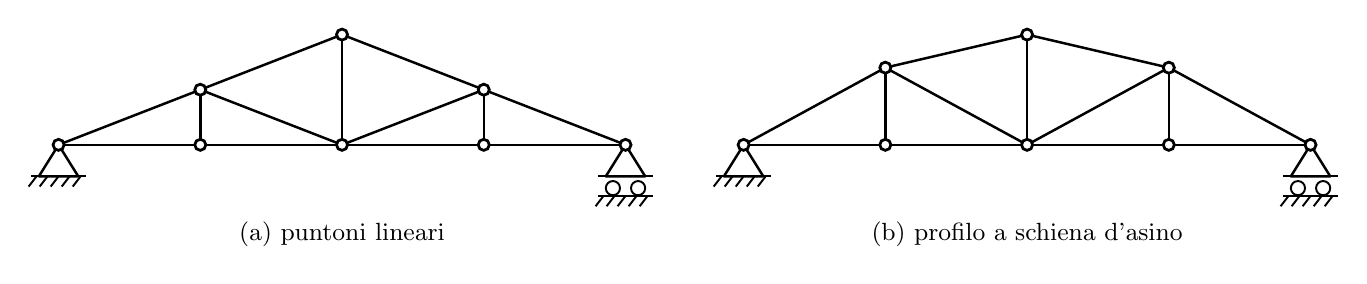
\begin{tikzpicture}[
			asta/.style={line width=0.90pt, line cap=round, line join=round, black},
			cord/.style={line width=0.90pt, line cap=round, line join=round, black},
			nodo/.style={circle, fill=white, draw=black,
				inner sep=0pt, minimum size=4pt, line width=1.0pt},
			terra/.style={line width=0.7pt, black},
			]
			\def\d{1.8}
			\def\hr{1.4}
			
			%% ── (a) puntoni lineari ────────────────────────────────
			\begin{scope}[xshift=0cm]
				\draw[cord](0,0)--(4*\d,0);
				\draw[cord](0,0)--(\d,{\hr/2})--(2*\d,\hr)--(3*\d,{\hr/2})--(4*\d,0);
				\draw[asta](2*\d,0)--(2*\d,\hr);
				\draw[asta](\d,0)--(\d,{\hr/2});
				\draw[asta](3*\d,0)--(3*\d,{\hr/2});
				\draw[asta](\d,{\hr/2})--(2*\d,0);
				\draw[asta](2*\d,0)--(3*\d,{\hr/2});
				\draw[cord](0,0)--(-0.25,-0.40)--(0.25,-0.40)--cycle;
				\draw[terra](-0.35,-0.40)--(0.35,-0.40);
				\foreach \xx in {-0.28,-0.14,0,0.14,0.28}
				\draw[terra](\xx,-0.40)--++(-0.10,-0.13);
				\draw[cord](4*\d,0)--(4*\d-0.25,-0.40)--(4*\d+0.25,-0.40)--cycle;
				\draw[terra](4*\d-0.35,-0.40)--(4*\d+0.35,-0.40);
				\draw[terra](4*\d-0.16,-0.55)circle(0.09);
				\draw[terra](4*\d+0.16,-0.55)circle(0.09);
				\draw[terra](4*\d-0.35,-0.65)--(4*\d+0.35,-0.65);
				\foreach \xx in {-0.28,-0.14,0,0.14,0.28}
				\draw[terra](4*\d+\xx,-0.65)--++(-0.10,-0.13);
				\foreach \x in {0,1,2,3,4} \node[nodo]at(\x*\d,0){};
				\node[nodo]at(\d,{\hr/2}){};
				\node[nodo]at(2*\d,\hr){};
				\node[nodo]at(3*\d,{\hr/2}){};
				\node[below,font=\small]at(2*\d,-0.85){(a) puntoni lineari};
			\end{scope}
			
			%% ── (b) profilo spezzato ───────────────────────────────
			\begin{scope}[xshift=8.7cm]
				\draw[cord](0,0)--(4*\d,0);
				\draw[cord](0,0)--(\d,{0.7*\hr})--(2*\d,\hr)--(3*\d,{0.7*\hr})--(4*\d,0);
				\draw[asta](2*\d,0)--(2*\d,\hr);
				\draw[asta](\d,0)--(\d,{0.7*\hr});
				\draw[asta](3*\d,0)--(3*\d,{0.7*\hr});
				\draw[asta](\d,{0.7*\hr})--(2*\d,0);
				\draw[asta](2*\d,0)--(3*\d,{0.7*\hr});
				\draw[cord](0,0)--(-0.25,-0.40)--(0.25,-0.40)--cycle;
				\draw[terra](-0.35,-0.40)--(0.35,-0.40);
				\foreach \xx in {-0.28,-0.14,0,0.14,0.28}
				\draw[terra](\xx,-0.40)--++(-0.10,-0.13);
				\draw[cord](4*\d,0)--(4*\d-0.25,-0.40)--(4*\d+0.25,-0.40)--cycle;
				\draw[terra](4*\d-0.35,-0.40)--(4*\d+0.35,-0.40);
				\draw[terra](4*\d-0.16,-0.55)circle(0.09);
				\draw[terra](4*\d+0.16,-0.55)circle(0.09);
				\draw[terra](4*\d-0.35,-0.65)--(4*\d+0.35,-0.65);
				\foreach \xx in {-0.28,-0.14,0,0.14,0.28}
				\draw[terra](4*\d+\xx,-0.65)--++(-0.10,-0.13);
				\foreach \x in {0,1,2,3,4} \node[nodo]at(\x*\d,0){};
				\node[nodo]at(\d,{0.7*\hr}){};
				\node[nodo]at(2*\d,\hr){};
				\node[nodo]at(3*\d,{0.7*\hr}){};
				\node[below,font=\small]at(2*\d,-0.85){(b) profilo a schiena d'asino};
			\end{scope}
			
	\end{tikzpicture}}
	\caption{Famiglie di maglie triangolari --- correnti spezzati
		(segue la \FIGref{fig:correnti_paralleli}).
		\emph{(d)}~Capriata a puntoni rettilinei: i nodi
		intermedi del corrente superiore giacciono sulla
		retta appoggio--colmo.
		\emph{(e)}~Profilo a schiena d'asino: i nodi
		intermedi sono al di sopra della retta di
		riferimento e il corrente superiore è
		genuinamente poligonale.}
	\label{fig:capriate_spezzato}
\end{figure}


\esottotit{Maglie romboidali.}
Nelle travature a maglie romboidali i pannelli
elementari hanno forma di rombo
(\FIGref{fig:tipologie_maglie}\,c), ottenuta con
correnti paralleli e diagonali incrociate (due per
pannello, disposte a X, secondo lo schema detto
anche \emph{a croce di Sant'Andrea})
Rispetto alle
maglie triangolari, ogni pannello ha un'asta in più;
la compatibilità con la condizione $n_a = 2n_n - 3$
è assicurata dal fatto che i nodi di intersezione
delle diagonali non sono nodi strutturali: le diagonali
si incrociano senza connessione.

Si noti il ruolo dell'unico montante $AB$: il
conteggio richiede esattamente un'asta verticale,
in assenza della quale la travatura risulterebbe
internamente labile di grado uno (e, con due
montanti, una volta iperstatica). Il montante
costituisce inoltre la maglia di innesco della
composizione gerarchica illustrata in figura,
circostanza che ne garantisce la non degenerazione;
la sua posizione lungo la travatura è invece
ininfluente ai fini della classificazione.

\esottotit{Maglie a K.}
Nelle travature a maglie a K i montanti verticali
incontrano le diagonali a metà altezza, dando al
pannello la caratteristica forma a K
(\FIGref{fig:tipologie_maglie}\,d). Lo schema è
stato adottato in alcune grandi travature da ponte,
anche ferroviarie, in cui la suddivisione del
pannello riduce la lunghezza libera delle diagonali
e quindi la loro sensibilità all'instabilità
(\CAPref{stabilita_travi} Vol.~III).

Anche qui un'asta particolare gioca il ruolo che
il montante $AB$ ha nelle maglie romboidali: il
montante centrale, l'unico privo del nodo di
mezzeria, deve restare intero perché il conteggio
si chiuda (spezzandolo con un nodo non raggiunto
da diagonali la travatura risulterebbe internamente
labile di grado uno). Esso costituisce la maglia
di innesco della composizione gerarchica illustrata
in figura; la sua collocazione al centro, dove le
diagonali invertono il verso, risponde a ragioni
statiche ed è invece ininfluente ai fini della
classificazione.

\esottotit{Generalizzazioni.}
Ulteriori evoluzioni geometriche si ottengono
sostituendo alcune aste di schemi triangolari o
romboidali con aste disposte diversamente, come
indicato nella \FIGref{fig:tipologie_maglie}\,e.
Questi schemi ibridi non si inquadrano in nessuna
delle famiglie precedenti ma obbediscono alla stessa
regola di isostaticità: la verifica di M\"{u}ller-Breslau
è la sola condizione generale applicabile.



\begin{oss}
	Il conteggio $n_a = 2n_n - 3$ è condizione
	\emph{necessaria} per l'isostaticità interna,
	ma non sufficiente. Come discusso nel
	\PARref{sec:composizione_degenerazioni},
	una travatura costruita per composizione
	gerarchica è automaticamente non degenere;
	per travature non costruite gerarchicamente
	(ad esempio quelle con maglie romboidali
	o ibride) occorre verificare l'assenza di
	degenerazioni geometriche.
\end{oss}


%............................................................................................................................
\subsection{Sistemi di travature: schemi complessi}
\label{subsec:sistemi_travature}
%............................................................................................................................

I sistemi articolati di corpi rigidi esaminati nella
Parte~II --- travi di Gerber, archi a tre cerniere,
sistemi sospesi --- danno luogo a sistemi reticolari
\emph{complessi} quando le singole travi componenti
vengono sostituite da travature reticolari. La
classificazione cinematica del sistema nel suo
complesso non muta, purché ciascuna travatura
componente sia internamente isostatica: la procedura
si articola in due fasi distinte.

La \emph{prima fase} è l'analisi locale di ciascuna
travatura componente, considerata isolatamente,
per verificarne l'isostaticità interna con la formula
di M\"{u}ller-Breslau. La \emph{seconda fase} è l'analisi
globale del sistema nel suo complesso, condotta con
i metodi della Parte~II per i sistemi di corpi rigidi,
trattando ciascuna travatura come un corpo rigido
equivalente. La sintesi delle due fasi dà il giudizio
definitivo.


%%%%%%%%%%%%%%%%%%%%%%%%%%%%%%%%%%%%%%%%%%%
\begin{figure}[!htbp]
	\centering
	\resizebox{\textwidth}{!}{%
		\begin{tikzpicture}[
			asta/.style={line width=0.9pt, line cap=round, line join=round, black},
			cord/.style={line width=1.8pt, line cap=round, line join=round, black},
			nodo/.style={circle, fill=white, draw=black,
				inner sep=0pt, minimum size=4.5pt, line width=0.9pt},
			etich/.style={font=\small},
			pan/.style={font=\small},
			]
			
			%% comandi per i vincoli -----------------------------------
			\newcommand{\cerniera}[1]{%
				\draw[line width=1.0pt](#1)--++(-0.24,-0.40)--++(0.48,0)--cycle;
				\draw[line width=1.0pt]($(#1)+(-0.34,-0.40)$)--($(#1)+(0.34,-0.40)$);
				\foreach \x in {-0.28,-0.14,0.00,0.14,0.28}
				\draw[very thin]($(#1)+(\x,-0.40)$)--++(-.10,-0.13);}
			\newcommand{\carrello}[1]{%
				\draw[line width=1.0pt](#1)--++(-0.24,-0.40)--++(0.48,0)--cycle;
				\draw[line width=1.0pt]($(#1)+(-0.34,-0.40)$)--($(#1)+(0.34,-0.40)$);
				\draw[line width=0.9pt]($(#1)+(-0.14,-0.49)$)circle(2.2pt);
				\draw[line width=0.9pt]($(#1)+( 0.14,-0.49)$)circle(2.2pt);
				\draw[line width=1.0pt]($(#1)+(-0.36,-0.58)$)--($(#1)+(0.36,-0.58)$);
				\foreach \x in {-0.28,-0.14,0.00,0.14,0.28}
				\draw[very thin]($(#1)+(\x,-0.58)$)--++(-.10,-0.13);}
			\newcommand{\pareteSX}[1]{%
				\draw[line width=1.0pt](#1)--++(-0.40,-0.24)--++(0,0.48)--cycle;
				\draw[line width=1.0pt]($(#1)+(-0.40,-0.34)$)--($(#1)+(-0.40,0.34)$);
				\foreach \yy in {-0.28,-0.14,0.00,0.14,0.28}
				\draw[very thin]($(#1)+(-0.40,\yy)$)--++(-0.13,-0.10);}
			\newcommand{\pareteDX}[1]{%
				\draw[line width=1.0pt](#1)--++(0.40,-0.24)--++(0,0.48)--cycle;
				\draw[line width=1.0pt]($(#1)+(0.40,-0.34)$)--($(#1)+(0.40,0.34)$);
				\foreach \yy in {-0.28,-0.14,0.00,0.14,0.28}
				\draw[very thin]($(#1)+(0.40,\yy)$)--++(0.13,0.10);}
			
			
			%% =========================================================
			%% (c) SCHEMA A TRE CERNIERE (cerniera in B, tolta l'asta CG)
			%% =========================================================
			\begin{scope}[xshift=0cm, yshift=-9.4cm]
				\def\db{1.6}
				\def\hb{1.1}
				%% corrente inferiore privo del tratto CG
				\draw[asta](0,0)--(2*\db,0);
				\draw[asta](3*\db,0)--(5*\db,0);
				%% corrente superiore completo
				\draw[asta](0.5*\db,\hb)--(4.5*\db,\hb);
				%% diagonali (Warren)
				\foreach \i in {0,...,4}{
					\draw[asta](\i*\db,0)--({(\i+0.5)*\db},\hb);
					\draw[asta]({(\i+0.5)*\db},\hb)--({(\i+1)*\db},0);}
				%% vincoli (in B cerniera al posto del carrello)
				\cerniera{0,0}
				\cerniera{5*\db,0}
				%% nodi
				\foreach \i in {0,...,5} \node[nodo]at(\i*\db,0){};
				\foreach \i in {0,...,4} \node[nodo]at({(\i+0.5)*\db},\hb){};
				%% etichette
				\node[etich,left ]at(-0.10,0.16){$A$};
				\node[etich,right]at(5*\db+0.10,0.16){$B$};
				\node[etich,below]at(2*\db,-0.10){$C$};
				\node[etich,below]at(3*\db,-0.10){$G$};
				\node[etich,above]at(2.5*\db,\hb+0.08){$D$};
			\end{scope}
			\node[pan]at(4.0,-11.30){(c)};
			
			%% =========================================================
			%% (d) TRAVATURA A MENSOLA CON TIRANTE
			%% =========================================================
			\begin{scope}[xshift=13.0cm, yshift=0cm]
				\def\h{0.95}
				%% correnti
				\draw[asta](0,0)--(11,0);
				\draw[asta](1,\h)--(12,\h);
				%% montanti e diagonali
				\foreach \i in {1,...,11} \draw[asta](\i,0)--(\i,\h);
				\foreach \i in {0,...,11} \draw[asta](\i,0)--(\i+1,\h);
				%% tirante a parete
				\coordinate (W) at (-0.9,2.5);
				\draw[asta](W)--(3,\h);
				\pareteSX{W}
				%% cerniera a terra
				\cerniera{0,0}
				%% nodi
				\foreach \i in {0,...,11} \node[nodo]at(\i,0){};
				\foreach \i in {1,...,12} \node[nodo]at(\i,\h){};
				\node[nodo]at(W){};
			\end{scope}
			
			\node[pan]at(19.5,-1.85){(d)};
			
			%% =========================================================
			%% (a) TRAVATURA RETICOLARE SEMPLICE CON ASTA DE
			%% =========================================================
			\begin{scope}[xshift=0cm, yshift=-0.1cm]
				\def\db{1.6}
				\def\hb{1.1}
				%% correnti
				\draw[asta](0,0)--(5*\db,0);
				\draw[asta](0.5*\db,\hb)--(4.5*\db,\hb);
				%% diagonali (Warren)
				\foreach \i in {0,...,4}{
					\draw[asta](\i*\db,0)--({(\i+0.5)*\db},\hb);
					\draw[asta]({(\i+0.5)*\db},\hb)--({(\i+1)*\db},0);}
				%% vincoli
				\cerniera{0,0}
				\carrello{5*\db,0}
				%% nodi
				\foreach \i in {0,...,5} \node[nodo]at(\i*\db,0){};
				\foreach \i in {0,...,4} \node[nodo]at({(\i+0.5)*\db},\hb){};
				%% etichette
				\node[etich,left ]at(-0.10,0.16){$A$};
				\node[etich,right]at(5*\db+0.10,0.16){$B$};
				\node[etich,below]at(2*\db,-0.10){$C$};
				\node[etich,above]at(2.5*\db,\hb+0.08){$D$};
				\node[etich,above]at(3.5*\db,\hb+0.08){$E$};
			\end{scope}
			\node[pan]at(4.0,-1.85){(a)};
			
			%% =========================================================
			%% (e) STRUTTURA SOSPESA, PRIMA VARIANTE
			%% =========================================================
			\begin{scope}[xshift=13.0cm, yshift=-5.1cm]
				\def\h{0.95}
				%% corrente inferiore (continuo: il tratto KM e' la biella)
				\draw[asta](0,0)--(12,0);
				%% corrente superiore interrotto fra H ed L
				\draw[asta](1,\h)--(6,\h);
				\draw[asta](7,\h)--(11,\h);
				%% montanti
				\foreach \i in {1,...,11} \draw[asta](\i,0)--(\i,\h);
				%% diagonali (soppressa quella della campata K-L)
				\foreach \i in {0,...,5} \draw[asta](\i,0)--(\i+1,\h);
				\foreach \i in {7,...,10} \draw[asta](\i,0)--(\i+1,\h);
				\draw[asta](11,\h)--(12,0);
				%% tiranti a parete
				\coordinate (W) at (-0.9,2.5);
				\draw[asta](W)--(3,\h);
				\pareteSX{W}
				\coordinate (V) at (13,2.5);
				\draw[asta](V)--(9,\h);
				\pareteDX{V}
				%% vincoli a terra
				\cerniera{0,0}
				\carrello{12,0}
				%% nodi
				\foreach \i in {0,...,12} \node[nodo]at(\i,0){};
				\foreach \i in {1,...,11} \node[nodo]at(\i,\h){};
				\node[nodo]at(W){};
				\node[nodo]at(V){};
				%% etichette
				\node[etich,above]at(6,\h+0.08){$H$};
				\node[etich,below]at(6,-0.10){$K$};
				\node[etich,above]at(7,\h+0.08){$L$};
				\node[etich,below]at(7,-0.10){$M$};
				\node[etich,above]at(8,\h+0.08){$N$};
				\node[etich,above left]at(9,\h+0.06){$C$};
				\node[etich,right]at(12.12,0.16){$B$};
				\node[etich,above left]at($(V)+(-0.10,-0.06)$){$D$};
			\end{scope}
			
			\node[pan]at(19.5,-6.85){(e)};
			
			%% =========================================================
			%% (b) TRAVATURA DI GERBER RETICOLARE
			%% =========================================================
			\begin{scope}[xshift=0cm, yshift=-5.1cm]
				\def\db{1.6}
				\def\hb{1.1}
				%% correnti (superiore privo del tratto DE)
				\draw[asta](0,0)--(5*\db,0);
				\draw[asta](0.5*\db,\hb)--(2.5*\db,\hb);
				\draw[asta](3.5*\db,\hb)--(4.5*\db,\hb);
				%% diagonali (Warren)
				\foreach \i in {0,...,4}{
					\draw[asta](\i*\db,0)--({(\i+0.5)*\db},\hb);
					\draw[asta]({(\i+0.5)*\db},\hb)--({(\i+1)*\db},0);}
				%% vincoli
				\cerniera{0,0}
				\carrello{2*\db,0}
				\carrello{5*\db,0}
				%% nodi
				\foreach \i in {0,...,5} \node[nodo]at(\i*\db,0){};
				\foreach \i in {0,...,4} \node[nodo]at({(\i+0.5)*\db},\hb){};
				%% etichette
				\node[etich,left ]at(-0.10,0.16){$A$};
				\node[etich,right]at(5*\db+0.10,0.16){$B$};
				\node[etich,right]at(2*\db+0.30,-0.18){$C$};
				\node[etich,above]at(2.5*\db,\hb+0.08){$D$};
				\node[etich,above]at(3.5*\db,\hb+0.08){$E$};
			\end{scope}
			\node[pan]at(4.0,-6.85){(b)};
			
			%% =========================================================
			%% (f) STRUTTURA SOSPESA, SECONDA VARIANTE
			%% =========================================================
			\begin{scope}[xshift=13.0cm, yshift=-9.4cm]
				\def\h{0.95}
				%% corrente inferiore interrotto fra K ed M
				\draw[asta](0,0)--(6,0);
				\draw[asta](7,0)--(12,0);
				%% corrente superiore interrotto fra E ed F e fra L ed N
				\draw[asta](1,\h)--(3,\h);
				\draw[asta](4,\h)--(7,\h);
				\draw[asta](8,\h)--(11,\h);
				%% montanti (L-M resta come pendolo di collegamento)
				\foreach \i in {1,...,11} \draw[asta](\i,0)--(\i,\h);
				%% diagonali (tutte presenti, stesso verso del pannello e)
				\foreach \i in {0,...,10} \draw[asta](\i,0)--(\i+1,\h);
				\draw[asta](11,\h)--(12,0);
				%% tiranti a parete
				\coordinate (W) at (-0.9,2.5);
				\draw[asta](W)--(3,\h);
				\pareteSX{W}
				\coordinate (V) at (13,2.5);
				\draw[asta](V)--(9,\h);
				\pareteDX{V}
				%% vincoli a terra (in B cerniera al posto del carrello)
				\cerniera{0,0}
				\cerniera{12,0}
				%% nodi
				\foreach \i in {0,...,12} \node[nodo]at(\i,0){};
				\foreach \i in {1,...,11} \node[nodo]at(\i,\h){};
				\node[nodo]at(W){};
				\node[nodo]at(V){};
				%% etichette
				\node[etich,above right]at(3,\h+0.04){$E$};
				\node[etich,above]at(4,\h+0.08){$F$};
				\node[etich,below]at(4,-0.10){$G$};
				\node[etich,above]at(6,\h+0.08){$H$};
				\node[etich,below]at(6,-0.10){$K$};
				\node[etich,above]at(7,\h+0.08){$L$};
				\node[etich,below]at(7,-0.10){$M$};
				\node[etich,above]at(8,\h+0.08){$N$};
				\node[etich,above left]at(9,\h+0.06){$C$};
				\node[etich,right]at(12.12,0.16){$B$};
				\node[etich,above left]at($(V)+(-0.10,-0.06)$){$D$};
			\end{scope}
			
			\node[pan]at(19.5,-11.30){(f)};
			
	\end{tikzpicture}}
	\caption{Sistemi reticolari complessi.
		\emph{(a)}: travatura reticolare semplicemente
		appoggiata, internamente isostatica.
		\emph{(b)}: travatura di Gerber reticolare,
		ottenuta sostituendo l'asta $DE$ del corrente
		superiore con un appoggio a carrello in $C$.
		\emph{(c)}: schema a tre cerniere, ottenuto
		sostituendo l'asta $CG$ del corrente inferiore
		con la componente orizzontale di reazione
		fornita dalla cerniera in $B$; il nodo $D$
		funge da cerniera interna fra le due travature.
		In entrambi i casi la classificazione cinematica
		globale è preservata.
		\emph{(d--f)}: strutture sospese ottenute
		dalla travatura a mensola per soppressione
		di aste interne e aggiunta di vincoli
		semplici equivalenti; le due varianti
		mostrano scelte diverse di aste soppresse
		e connessioni introdotte.}
	\label{fig:sistemi_complessi}
\end{figure}
%%%%%%%%%%%%%%%%%%%%%%%%%%%%%%%%%%%%%%%%%%%

\esottotit{Travatura di Gerber reticolare.}
La travatura reticolare semplicemente appoggiata di
\FIGref{fig:sistemi_complessi}\,(a) è internamente
isostatica per composizione gerarchica. La sostituzione
dell'asta $DE$ del corrente superiore con un appoggio
a carrello in $C$ produce la \emph{travatura di Gerber
	reticolare} di \FIGref{fig:sistemi_complessi}\,(b).
L'operazione --- rimozione di un'asta interna e
aggiunta di un vincolo esterno semplice equivalente
--- preserva la classificazione cinematica globale.
Questo è il \emph{principio di sostituzione
	asta--vincolo}, discusso formalmente nel
\PARref{sec:sostituzione_reticolari}.


\esottotit{Schema a tre cerniere.}
Dalla stessa travatura di \FIGref{fig:sistemi_complessi}\,(a)
si ottiene lo schema di \FIGref{fig:sistemi_complessi}\,(c)
sopprimendo l'asta $CG$ del corrente inferiore e
sostituendo il carrello in $B$ con una cerniera:
l'asta orizzontale soppressa è rimpiazzata dalla
componente orizzontale di reazione che la cerniera
aggiunge. Le due travature parziali restano collegate
nel nodo $D$, che funge da cerniera interna: il sistema
è l'analogo reticolare dell'arco a tre cerniere
(\PARref{subsec:tre_cerniere} del
\CAPref{cap:assemblaggi_travi}), con le cerniere in
$A$, $D$ e $B$ non allineate. La scelta dell'asta da
sopprimere non è indifferente: rimuovendo nuovamente
$DE$, la cerniera interna cadrebbe sul corrente
inferiore, allineata con $A$ e $B$, e lo schema
risulterebbe degenere.


\esottotit{Strutture sospese.}
Lo schema di \FIGref{fig:sistemi_complessi}\,(d) mostra
una travatura a mensola sorretta da una cerniera e da
un tirante ancorato in alto. Le strutture sospese di
\FIGref{fig:sistemi_complessi}\,(e)--(f) nascono dalla
combinazione degli stessi ingredienti su una travatura
appoggiata di dodici campi, analoga a quella dello
schema (a): nello schema (e) si aggiungono due tiranti
e si sopprimono due aste (il tratto $HL$ del corrente
superiore e la diagonale $KL$), sicché le due travature
parziali restano collegate dalla biella inferiore $KM$;
nello schema (f) si aggiungono i due tiranti, si
sostituisce il carrello in $B$ con una cerniera e si
sopprimono tre aste (i tratti $EF$ ed $LN$ del corrente
superiore e il tratto $KM$ di quello inferiore), sicché
il montante $LM$ resta a fare da pendolo di collegamento.
In ogni caso ciascuna asta soppressa è compensata da un
vincolo semplice aggiunto: la classificazione globale
del sistema rimane invariata, come si verifica applicando
la formula di M\"{u}ller-Breslau all'intero sistema o
decomponendo il problema nelle due fasi descritte sopra.










\begin{oss}
	Il principio di sostituzione asta--vincolo
	ha un ruolo centrale nella progettazione
	concettuale: esso mostra che la classificazione
	cinematica di una travatura non dipende dalla
	specifica scelta delle aste e dei vincoli, ma
	dalla loro \emph{numerosità e posizione}. Due
	travature con disposizioni molto diverse di
	aste e vincoli possono essere cinematicamente
	equivalenti, e dunque scambiabili nella
	modellazione senza alterare il grado di
	determinazione del sistema.
\end{oss}



%..............................................................
\subsection{Cenni alle travature reticolari spaziali}
\label{subsec:reticolari_spaziali}
%..............................................................

Il passaggio dalle strutture piane a quelle spaziali
amplia le possibilità di aggregazione delle aste,
ma non altera la logica di classificazione: la
formula di M\"{u}ller-Breslau nel caso spaziale diventa
\begin{equation}\label{eq:muller_breslau_spaz}
	\nu = 3n_n - n_a - m_{\text{est}},
\end{equation}
con $3n_n$ gradi di libertà traslazionali dei nodi
(tre componenti per nodo) e la condizione di
isostaticità interna $n_a = 3n_n - 6$ (contro
$n_a = 2n_n - 3$ nel caso piano). Gli schemi della \FIGref{fig:reticolari_spaz} illustrano
le famiglie principali a titolo di orientamento;
la loro analisi dettagliata esula dagli obiettivi
del presente volume, essendo oggetto dei corsi
di progettazione strutturale.

\esottotit{Elemento tetraedrico e composizione ricorrente.}
L'elemento base delle travature spaziali isostatiche
è il \emph{tetraedro}: quattro nodi collegati da
sei aste, che soddisfa $n_a = 6 = 3 \times 4 - 6
= 3n_n - 6$. La composizione ricorrente avviene
aggiungendo ad ogni passo un nodo e tre aste nuove,
conservando la condizione di isostaticità interna
ad ogni passo. Così, a partire dal tetraedro base
$ABCD$, si generano gli elementi $ABCDE$,
$ABCDEF$, $ABCDEFG$ e così via, come illustrato
nella \FIGref{fig:reticolari_spaz}\,a.


\esottotit{Travature a moduli tetraedrici: svincolamento esterno.}
Gli schemi (b) e (c) di \FIGref{fig:reticolari_spaz}
mostrano la stessa travatura spaziale --- costruita
per aggregazione di moduli tetraedrici ---
con due diversi dispositivi di vincolamento
esterno, entrambi isostatici.

Nello schema (b) i vincoli al suolo sono una cerniera
sferica all'estremità sinistra, due pendoli verticali
disposti simmetricamente ai nodi dei due correnti
inferiori all'estremità destra, e un pendolo orizzontale
applicato alla stessa estremità destra: la cerniera
sferica impone tre condizioni di vincolo cinematico
bloccando tutte e tre le traslazioni all'estremità
sinistra; i due pendoli verticali, agendo in punti
lateralmente separati, bloccano la rotazione di
beccheggio attorno all'asse trasversale e la rotazione
di rollio attorno all'asse longitudinale; il pendolo
orizzontale, orientato trasversalmente, blocca la
rotazione di imbardata attorno all'asse verticale.
Il totale è $m_{\text{est}} = 3 + 2 + 1 = 6$ vincoli
semplici, sufficiente per l'isostaticità esterna a
condizione che il pendolo orizzontale non sia orientato
parallelamente all'asse longitudinale, direzione già
vincolata dalla cerniera sferica.


Nello schema (c) i vincoli sono: una cerniera sferica
in un nodo dell'estremità sinistra, due pendoli
convergenti in un nodo dell'estremità destra e un
tirante, ancorato in alto, applicato a un secondo
nodo dell'estremità sinistra. La cerniera sferica
blocca le tre traslazioni del nodo cui è applicata:
i moti rigidi residui sono le sole rotazioni attorno
ad assi passanti per quel nodo, tre componenti in
tutto. I due pendoli convergenti ne sopprimono due:
l'unico moto residuo è la rotazione attorno all'asse
che congiunge il nodo della cerniera sferica con il
nodo dei pendoli, rotazione che lascia fermi entrambi
i nodi vincolati (purché i due pendoli e l'asse non
giacciano in uno stesso piano). È il tirante --- la
cui retta d'azione è sghemba rispetto a quell'asse,
non incontrandolo e non essendogli parallela, e
possiede dunque momento non nullo rispetto ad esso ---
a bloccare quest'ultimo modo di spostamento rigido,
portando il totale a
$m_{\text{est}} = 3 + 2 + 1 = 6$ vincoli semplici
e rendendo il sistema isostatico esternamente.

I due schemi condividono dunque la medesima struttura
logica: una cerniera sferica (tre condizioni), una
coppia di pendoli (due condizioni) e una sesta asta
destinata a sopprimere l'unica rotazione residua,
attorno a un asse passante per la cerniera sferica.
Cambia soltanto la disposizione: in (b) i pendoli,
applicati a nodi distinti, lasciano libera la
rotazione attorno all'asse verticale per la cerniera,
soppressa dal pendolo trasversale; in (c) i pendoli,
convergenti in un nodo, lasciano libera la rotazione
attorno alla congiungente fra la cerniera e quel nodo,
soppressa dal tirante. In entrambi i casi la condizione
di efficacia è la stessa: la sesta asta deve possedere
momento non nullo rispetto all'asse della rotazione
residua.

%%%%%%%%%%%%%%%%%%%%%%%%%%%%%%%%%%%%%%%%%%%
\begin{figure}[!htbp]
	\centering
	\resizebox{\textwidth}{!}{%
		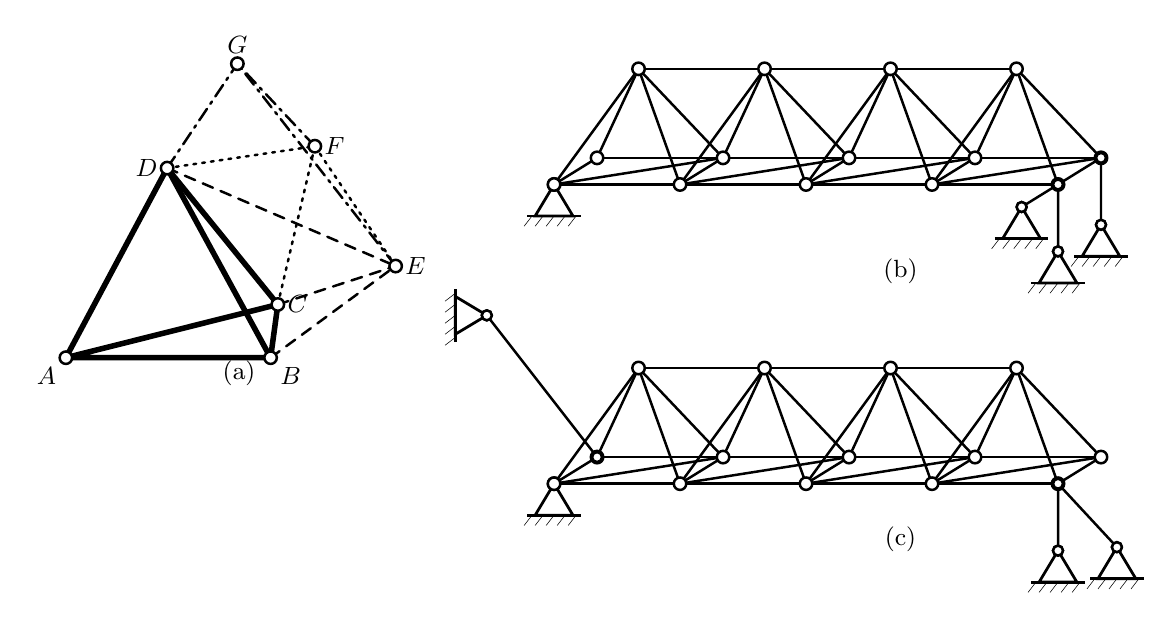
\begin{tikzpicture}[
			asta/.style={line width=0.9pt, line cap=round, line join=round, black},
			base/.style={line width=2.0pt, line cap=round, line join=round, black},
			nuova/.style={line width=0.9pt, line cap=round, line join=round, black,
				dash pattern=on 4pt off 3pt},
			futura/.style={line width=0.9pt, line cap=round, black,
				dash pattern=on 1pt off 2.2pt},
			quarta/.style={line width=0.9pt, line cap=round, black,
				dash pattern=on 5pt off 2.2pt on 1pt off 2.2pt},
			nodo/.style={circle, fill=white, draw=black,
				inner sep=0pt, minimum size=4.5pt, line width=0.9pt},
			etich/.style={font=\small},
			pan/.style={font=\small},
			assi/.style={x={(1cm,0cm)}, y={(0.42cm,0.26cm)}, z={(0cm,1cm)}},
			]
			
			%% simboli di vincolo --------------------------------
			\newcommand{\cerniera}[1]{%
				\begin{scope}[shift={(#1)}, x={(1cm,0cm)}, y={(0cm,1cm)}]
					\draw[line width=1.0pt](0,0)--(-0.24,-0.40)--(0.24,-0.40)--cycle;
					\draw[line width=1.0pt](-0.34,-0.40)--(0.34,-0.40);
					\foreach \x in {-0.28,-0.14,0.00,0.14,0.28}
					\draw[very thin](\x,-0.40)--++(-.10,-0.13);
			\end{scope}}
			\newcommand{\pareteSX}[1]{%
				\begin{scope}[shift={(#1)}, x={(1cm,0cm)}, y={(0cm,1cm)}]
					\draw[line width=1.0pt](0,0)--(-0.40,-0.24)--(-0.40,0.24)--cycle;
					\draw[line width=1.0pt](-0.40,-0.34)--(-0.40,0.34);
					\foreach \yy in {-0.28,-0.14,0.00,0.14,0.28}
					\draw[very thin](-0.40,\yy)--++(-0.13,-0.10);
			\end{scope}}
			%% pendolo: biella da #1 a #2 con cerniere agli estremi
			\newcommand{\pendolo}[2]{%
				\draw[asta](#1)--(#2);
				\node[nodo, minimum size=3.6pt]at(#1){};
				\node[nodo, minimum size=3.6pt]at(#2){};}
			
			%% =========================================================
			%% (a) COMPOSIZIONE RICORRENTE DAL TETRAEDRO ABCD
			%% =========================================================
			\begin{scope}[assi, xshift=0cm, yshift=-0.8cm]
				\coordinate (A) at (0,0,0);
				\coordinate (B) at (2.6,0,0);
				\coordinate (C) at (1.6,2.6,0);
				\coordinate (D) at (0.95,0.8,2.2);
				\coordinate (E) at (3.6,1.4,0.8);
				\coordinate (F) at (2.7,1.1,2.4);
				\coordinate (G) at (1.8,0.9,3.5);
				%% tetraedro base
				\draw[base](A)--(B)--(C)--cycle;
				\draw[base](A)--(D);
				\draw[base](B)--(D);
				\draw[base](C)--(D);
				%% nodo E (tre aste nuove)
				\draw[nuova](B)--(E);
				\draw[nuova](C)--(E);
				\draw[nuova](D)--(E);
				%% nodo F
				\draw[futura](C)--(F);
				\draw[futura](D)--(F);
				\draw[futura](E)--(F);
				%% nodo G
				\draw[quarta](D)--(G);
				\draw[quarta](E)--(G);
				\draw[quarta](F)--(G);
				\foreach \n in {A,B,C,D,E,F,G} \node[nodo]at(\n){};
				\node[etich,below left ]at(A){$A$};
				\node[etich,below right]at(B){$B$};
				\node[etich,right]at(C){$C$};
				\node[etich,left       ]at(D){$D$};
				\node[etich,right      ]at(E){$E$};
				\node[etich,right      ]at(F){$F$};
				\node[etich,above      ]at(G){$G$};
			\end{scope}
			\node[pan]at(2.2,-1.0){(a)};
			
			%% =========================================================
			%% travatura a moduli tetraedrici (geometria comune b-c)
			%% =========================================================
			\newcommand{\boomtetra}{%
				%% correnti inferiori
				\draw[asta](L0)--(L4);
				\draw[asta](R0)--(R4);
				%% corrente superiore
				\draw[asta](T0)--(T3);
				%% piano inferiore: traversi e diagonali
				\foreach \i in {0,...,4} \draw[asta](L\i)--(R\i);
				\foreach \i [evaluate=\i as \j using int(\i+1)] in {0,...,3}
				\draw[asta](L\i)--(R\j);
				%% aste di parete
				\foreach \i [evaluate=\i as \j using int(\i+1)] in {0,...,3}{
					\draw[asta](T\i)--(L\i);
					\draw[asta](T\i)--(R\i);
					\draw[asta](T\i)--(L\j);
					\draw[asta](T\i)--(R\j);}
				%% nodi
				\foreach \i in {0,...,4}{\node[nodo]at(L\i){};\node[nodo]at(R\i){};}
				\foreach \i in {0,...,3} \node[nodo]at(T\i){};}
			
			\newcommand{\boomcoord}{%
				\foreach \i in {0,...,4}{
					\coordinate (L\i) at (1.6*\i,0,0);
					\coordinate (R\i) at (1.6*\i,1.3,0);}
				\foreach \i in {0,...,3}
				\coordinate (T\i) at (1.6*\i+0.8,0.65,1.3);}
			
			%% =========================================================
			%% (b) PRIMO SCHEMA DI VINCOLO
			%% =========================================================
			\begin{scope}[assi, xshift=6.2cm, yshift=1.4cm]
				\boomcoord
				\boomtetra
				%% cerniera sferica a sinistra (nodo L0)
				\cerniera{L0}
				%% pendoli verticali ai due correnti inferiori (L4, R4)
				\coordinate (pL) at (6.4,0,-0.85);
				\coordinate (pR) at (6.4,1.3,-0.85);
				\pendolo{L4}{pL} \cerniera{pL}
				\pendolo{R4}{pR} \cerniera{pR}
				%% pendolo orizzontale trasversale (da L4)
				\coordinate (pT) at (6.4,-1.1,0);
				\pendolo{L4}{pT} \cerniera{pT}
				%% anellini ridisegnati sopra i vincoli
				\node[nodo]at(L0){};
				\foreach \p in {pL,pR,pT} \node[nodo, minimum size=3.6pt]at(\p){};
			\end{scope}
			\node[pan]at(10.6,0.30){(b)};
			
			%% =========================================================
			%% (c) SECONDO SCHEMA DI VINCOLO
			%% =========================================================
			\begin{scope}[assi, xshift=6.2cm, yshift=-2.4cm]
				\boomcoord
				\boomtetra
				%% cerniera sferica a sinistra (nodo L0)
				\cerniera{L0}
				%% tirante dall'alto al secondo nodo di sinistra (R0)
				\coordinate (bW) at (-1.4,1.3,1.8);
				\pendolo{bW}{R0} \pareteSX{bW}
				%% due pendoli convergenti nel nodo L4
				\coordinate (q1) at (6.4,0,-0.85);
				\coordinate (q2) at (7.4,-0.6,-0.65);
				\pendolo{L4}{q1} \cerniera{q1}
				\pendolo{L4}{q2} \cerniera{q2}
				%% anellini ridisegnati sopra i vincoli
				\node[nodo]at(L0){};
				\foreach \p in {bW,q1,q2} \node[nodo, minimum size=3.6pt]at(\p){};
			\end{scope}
			\node[pan]at(10.6,-3.1){(c)};
			
	\end{tikzpicture}}
	\caption{Travature reticolari spaziali.
		\emph{(a)}: composizione ricorrente dal tetraedro
		base $ABCD$; ad ogni passo si aggiunge un nodo
		e tre aste (tratteggiate), generando gli elementi
		$ABCDE$, $ABCDEF$, $ABCDEFG$.
		\emph{(b)}: travatura a moduli tetraedrici con
		schema di vincolo esterno isostatico ($m_{\text{est}} = 6$):
		cerniera sferica all'estremità sinistra, due pendoli
		verticali ai nodi dei correnti inferiori e un pendolo
		orizzontale trasversale all'estremità destra.
		\emph{(c)}: stessa travatura con schema di vincolo
		esterno alternativo ($m_{\text{est}} = 6$): cerniera
		sferica all'estremità sinistra, tirante dall'alto al
		secondo nodo della stessa estremità, due pendoli
		convergenti all'estremità destra; il tirante blocca
		la rotazione attorno all'asse congiungente la cerniera
		sferica con il punto di intersezione dei due pendoli.}
	\label{fig:reticolari_spaz}
\end{figure}
%%%%%%%%%%%%%%%%%%%%%%%%%%%%%%%%%%%%%%%%%%%


%%%%%%%%%%%%%%%%%%%%%%%%%%%%%%%%%%%%%%%%%%%
\begin{figure}[htbp]
	\centering
	\resizebox{\textwidth}{!}{%
		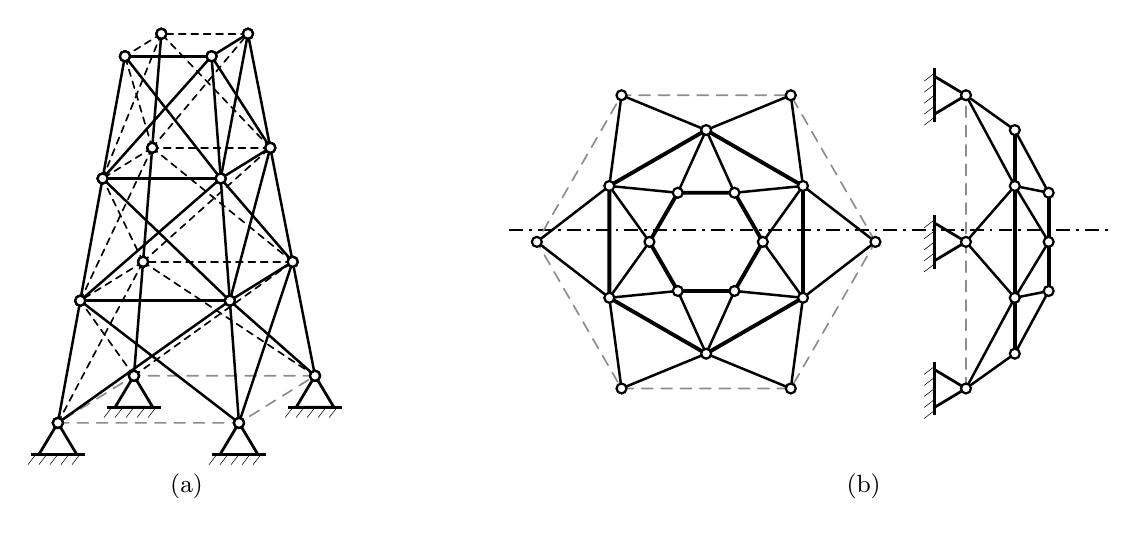
\begin{tikzpicture}[
			asta/.style={line width=0.9pt, line cap=round, line join=round, black},
			anello/.style={line width=1.4pt, line cap=round, line join=round, black},
			anellobase/.style={line width=0.6pt, line cap=round, black!45,	dash pattern=on 4pt off 3pt},
			nascosta/.style={line width=0.6pt, line cap=round, black,dash pattern=on 2.5pt off 2pt},
			assesim/.style={line width=0.6pt,dash pattern=on 5pt off 2.2pt on 1pt off 2.2pt},
			nodo/.style={circle, fill=white, draw=black, inner sep=0pt, minimum size=4.5pt, line width=0.9pt},
			nodino/.style={circle, fill=white, draw=black,	inner sep=0pt, minimum size=3.6pt, line width=0.8pt},
			etich/.style={font=\small},
			pan/.style={font=\small},
			assi/.style={x={(1cm,0cm)}, y={(0.42cm,0.26cm)}, z={(0cm,1cm)}},
			]
			
			\newcommand{\cerniera}[1]{%
				\begin{scope}[shift={(#1)}, x={(1cm,0cm)}, y={(0cm,1cm)}]
					\draw[line width=1.0pt](0,0)--(-0.24,-0.40)--(0.24,-0.40)--cycle;
					\draw[line width=1.0pt](-0.34,-0.40)--(0.34,-0.40);
					\foreach \x in {-0.28,-0.14,0.00,0.14,0.28}
					\draw[very thin](\x,-0.40)--++(-.10,-0.13);
			\end{scope}}
			\newcommand{\pareteSX}[1]{%
				\begin{scope}[shift={(#1)}, x={(1cm,0cm)}, y={(0cm,1cm)}]
					\draw[line width=1.0pt](0,0)--(-0.40,-0.24)--(-0.40,0.24)--cycle;
					\draw[line width=1.0pt](-0.40,-0.34)--(-0.40,0.34);
					\foreach \yy in {-0.28,-0.14,0.00,0.14,0.28}
					\draw[very thin](-0.40,\yy)--++(-0.13,-0.10);
			\end{scope}}
			\newcommand{\cernieraV}[1]{%
				\begin{scope}[shift={(#1)}, x={(1cm,0cm)}, y={(0cm,1cm)}]
					\draw[line width=1.0pt](0,0)--(-0.40,-0.24)--(-0.40,0.24)--cycle;
					\draw[line width=1.0pt](-0.40,-0.34)--(-0.40,0.34);
					\foreach \yy in {-0.28,-0.14,0.00,0.14,0.28}
					\draw[very thin](-0.40,\yy)--++(-0.13,-0.10);
			\end{scope}}
			
			%% =========================================================
			%% (a) PILONE RETICOLARE A PIANTA QUADRATA
			%% =========================================================
			\begin{scope}[assi, xshift=0cm, yshift=0cm]
				%% livelli: z e semilarghezze
				\foreach \k/\z/\a in {0/0.0/1.15, 1/1.5/0.95, 2/3.0/0.75, 3/4.5/0.55}{
					\coordinate (A\k) at (-\a,-\a,\z);
					\coordinate (B\k) at ( \a,-\a,\z);
					\coordinate (C\k) at ( \a, \a,\z);
					\coordinate (D\k) at (-\a, \a,\z);}
				%% base (in pianta, nascosta)
				\draw[anellobase](A0)--(B0)--(C0)--(D0)--cycle;
				%% montanti angolari
				\foreach \p in {A,B,C,D}
				\draw[asta](\p0)--(\p1)--(\p2)--(\p3);
				%% traversi ai livelli 1..3
				\foreach \k in {1,2,3}{
					\draw[asta](A\k)--(B\k);
					\draw[asta](B\k)--(C\k);
					\draw[nascosta](C\k)--(D\k);
					\draw[nascosta](D\k)--(A\k);}
				%% controventi a X: facce anteriori in vista
				\foreach \k [evaluate=\k as \j using int(\k+1)] in {0,1,2}{
					\draw[asta](A\k)--(B\j);
					\draw[asta](B\k)--(A\j);
					\draw[asta](B\k)--(C\j);
					\draw[asta](C\k)--(B\j);
					\draw[nascosta](C\k)--(D\j);
					\draw[nascosta](D\k)--(C\j);
					\draw[nascosta](D\k)--(A\j);
					\draw[nascosta](A\k)--(D\j);}
				%% vincoli al suolo
				\foreach \p in {A,B,C,D} \cerniera{\p0}
				%% nodi (ridisegnati sopra i vincoli)
				\foreach \k in {0,1,2,3}
				\foreach \p in {A,B,C,D}
				\node[nodino]at(\p\k){};
			\end{scope}
			
			%% =========================================================
			%% (b) CUPOLA RETICOLARE: PIANTA E PROSPETTO RIBALTATO
			%%     (asse orizzontale comune; le ordinate dei nodi della
			%%     pianta coincidono con quelle del prospetto)
			%% =========================================================
			%% asse comune
			\draw[assesim](4.10,2.15)--(11.70,2.15);
			
			%% ---- pianta (perimetro con vertici a 0+60k) ----
			\begin{scope}[xshift=6.6cm, yshift=2.0cm]
				\foreach \k in {0,...,5}{
					\coordinate (P\k) at ({60*\k}:0.72);
					\coordinate (Q\k) at ({60*\k+30}:1.42);
					\coordinate (R\k) at ({60*\k}:2.15);}
				%% anelli interni
				\draw[anello](P0)--(P1)--(P2)--(P3)--(P4)--(P5)--cycle;
				\draw[anello](Q0)--(Q1)--(Q2)--(Q3)--(Q4)--(Q5)--cycle;
				%% anello perimetrale (tratteggiato: sostituibile dai vincoli)
				\draw[anellobase] (R0)--(R1)--(R2)--(R3)--(R4)--(R5)--cycle;
				%% rete antiprismatica fra gli anelli
				\foreach \k [evaluate=\k as \j using {int(mod(\k+1,6))}] in {0,...,5}{
					\draw[asta](Q\k)--(P\k);
					\draw[asta](Q\k)--(P\j);
					\draw[asta](R\k)--(Q\k);
					\draw[asta](R\j)--(Q\k);}
				%% nodi
				\foreach \k in {0,...,5}{
					\node[nodino]at(P\k){}; \node[nodino]at(Q\k){};
					\node[nodino]at(R\k){};}
			\end{scope}
			
			%% ---- prospetto ribaltato a destra ----
			\begin{scope}[xshift=9.9cm, yshift=2.0cm]
				%% traccia (tratteggiata) dell'anello perimetrale: linea d'imposta
				\draw[anellobase](0,-1.862)--(0,1.862);
				%\draw[anello, dash pattern=on 4pt off 3pt](0,-1.862)--(0,1.862);
				%% tracce degli anelli intermedi e di sommita'
				\draw[anello](0.62,-1.42)--(0.62,1.42);
				\draw[anello](1.05,-0.624)--(1.05,0.624);
				%% rete fra perimetro e secondo anello
				\draw[asta](0,1.862)--(0.62,1.42);
				\draw[asta](0,1.862)--(0.62,0.71);
				\draw[asta](0,0)--(0.62,0.71);
				\draw[asta](0,0)--(0.62,-0.71);
				\draw[asta](0,-1.862)--(0.62,-0.71);
				\draw[asta](0,-1.862)--(0.62,-1.42);
				%% rete fra secondo anello e anello di sommita'
				\draw[asta](0.62,1.42)--(1.05,0.624);
				\draw[asta](0.62,0.71)--(1.05,0.624);
				\draw[asta](0.62,0.71)--(1.05,0);
				\draw[asta](0.62,-0.71)--(1.05,0);
				\draw[asta](0.62,-0.71)--(1.05,-0.624);
				\draw[asta](0.62,-1.42)--(1.05,-0.624);
				%% vincoli sulla linea d'imposta
				\cernieraV{0,1.862}
				\cernieraV{0,0}
				\cernieraV{0,-1.862}
				%% nodi
				
				\foreach \p in {(0,-1.862),(0,0),(0,1.862),
					(0.62,-1.42),(0.62,-0.71),(0.62,0.71),(0.62,1.42),
					(1.05,-0.624),(1.05,0),(1.05,0.624)}
				\node[nodino]at\p{};
			\end{scope}
			
			\node[pan]at(0,-1.1){(a)};
			\node[pan]at(8.6,-1.1){(b)};
			
	\end{tikzpicture}}
	\caption{Piloni e cupole reticolari.
		\emph{(a)}: pilone verticale reticolare a pianta
		quadrata, ottenuto per sovrapposizione di conci
		a pianta quadrangolare; i vincoli al suolo sono
		indicati alle basi dei montanti angolari.
		\emph{(b)}: cupola reticolare; al centro la pianta
		con la rete di nodi e aste, a destra il prospetto,
		ribaltato attorno alla linea d'imposta, con
		l'andamento della calotta, le aste di parete in
		proiezione, le tracce degli anelli e i vincoli di
		appoggio al perimetro; pianta e prospetto sono
		allineati sullo stesso asse.
		L'anello perimetrale, tratteggiato, può essere
		omesso quando i vincoli di appoggio bloccano
		tutti i nodi del perimetro.}
	\label{fig:piloni_cupole}
\end{figure}
%%%%%%%%%%%%%%%%%%%%%%%%%%%%%%%%%%%%%%%%%%%


\esottotit{Piloni reticolari.}
Sovrapponendo conci strutturali a pianta
quadrangolare si ottiene un \emph{pilone verticale
	reticolare} (\FIGref{fig:piloni_cupole}\,(a)).
La simmetria del sistema richiede particolare
attenzione nella scelta dei vincoli al suolo:
una disposizione troppo simmetrica può lasciare
libera la rotazione d'insieme attorno all'asse
verticale, producendo un meccanismo rigido anche
quando il conteggio di M\"{u}ller-Breslau dà $\nu = 0$.
Lo schema è generalizzabile a piante poligonali
(piloni pentagonali, esagonali) e, al limite, a
geometrie circolari.

\esottotit{Cupole reticolari.}
Quando il poligono di sommità è molto più piccolo
del poligono di base, i conci a pianta poligonale
danno luogo a \emph{strutture a cupola}
(\FIGref{fig:piloni_cupole}\,(b)). La cupola
reticolare è la versione discreta della calotta
sferica e trova impiego in coperture di grandi
luci. La rete di aste si genera coordinando anelli
orizzontali e meridiani: la pianta mostra la
disposizione planimetrica dei nodi, la sezione
laterale l'andamento della calotta.



\begin{oss}
	Il confronto tra gli schemi b) e c) evidenzia
	una differenza qualitativa rispetto al caso
	piano: in tre dimensioni i gradi di libertà
	rotazionali del corpo rigido sono tre
	(non uno solo), e la condizione $m_{\text{est}} = 6$
	necessaria per l'isostaticità esterna non
	garantisce automaticamente che tutti e sei i
	moti rigidi siano contrastati. La verifica
	geometrica --- analoga alla condizione di
	non allineamento dei vincoli nel caso piano ---
	diventa in tre dimensioni non banale e
	richiede l'esame esplicito dei modi di
	spostamento rigido.
\end{oss}



%----------------------------------------------------------------------------------------------------------------------------
\section{Composizione gerarchica e degenerazioni geometriche}
\label{sec:composizione_degenerazioni}
%----------------------------------------------------------------------------------------------------------------------------

La composizione gerarchica caratterizza le travature
isostatiche e ne garantisce la stabilità geometrica
ad ogni passo costruttivo; le degenerazioni
geometriche rappresentano invece le eccezioni in
cui il conteggio di M\"{u}ller-Breslau non è sufficiente
a garantire l'isostaticità effettiva. Entrambi gli
aspetti vengono discussi nelle sottosezioni che
seguono con riferimento agli schemi piani, che
costituiscono il tema centrale del capitolo.

%............................................................................................................................
\subsection{Travature isostatiche e composizione
	gerarchica}
\label{subsec:reticolari_isostatiche}
%............................................................................................................................

La condizione di isostaticità interna $n_a = 2n_n - 3$
e la procedura di composizione gerarchica --- partendo
da un triangolo base e aggiungendo ciascun nuovo nodo
con due aste nuove --- sono state introdotte e
dimostrate nel \PARref{sec:muller_breslau_classificazione}
(\FIGref{fig:reticolare_gerarchia}).

Qui interessa la conseguenza operativa: la struttura
gerarchica suggerisce un ordine naturale di risoluzione.
Il nodo aggiunto per ultimo è collegato a soli due
nodi precedenti da due aste, ed è quindi il primo
ad essere risolvibile una volta note le reazioni
esterne. Risalendo la gerarchia in ordine inverso,
ogni nodo si trova nella stessa condizione nel
momento in cui viene affrontato. Questo è il
fondamento del metodo dei nodi, sviluppato nel
\PARref{sec:metodo_nodi}.


%............................................................................................................................
\subsection{Travature iperstatiche e degenerazioni
	geometriche}
\label{subsec:reticolari_iperstatiche}
%............................................................................................................................

Quando $\nu < 0$ la travatura è sovradeterminata.
Come sarà discusso nel \PARref{sec:classificazione_reticolari},
la sovradeterminazione può essere esterna
($g_\text{est} = m_\text{est} - 3 > 0$) o interna
($g_\text{int} = n_a - (2n_n - 3) > 0$), o entrambe.
In entrambi i casi la formula di M\"{u}ller-Breslau
fornisce il valore corretto di $\nu$ purché le
equazioni di vincolo siano \emph{linearmente
	indipendenti}: quando questa condizione viene meno
si producono \emph{degenerazioni geometriche} che
alterano il comportamento reale della struttura
rispetto a quanto previsto dal conteggio.

\esottotit{Degenerazioni nodali.}
La degenerazione più comune è quella nodale: due
o più aste convergenti in un nodo sono allineate
lungo la stessa retta. In questo caso le equazioni
di equilibrio del nodo nelle due direzioni del piano
non sono indipendenti nella direzione trasversale
alle aste allineate: le aste parallele non possono
equilibrare forze perpendicolari al loro comune
asse, e il nodo ammette un moto di scorrimento
trasversale anche se il conteggio di M\"{u}ller-Breslau
darebbe $\nu = 0$.

La degenerazione nodale è riconoscibile per ispezione
geometrica: è sufficiente verificare che in ogni
nodo le aste convergenti non siano tutte parallele
a una stessa direzione. La condizione di
\emph{non degenerazione} richiede che in ogni nodo
esistano almeno due aste con direzioni linearmente
indipendenti.

\esottotit{Degenerazioni globali.}
Esistono configurazioni in cui nessun singolo nodo
presenta allineamenti locali, ma la struttura nel
suo insieme ammette meccanismi geometrici. Questi
si verificano quando sottostrutture --- gruppi di
aste e nodi --- si comportano come un corpo rigido
con un grado di libertà interno, pur rispettando
il conteggio globale di M\"{u}ller-Breslau.

Il test del moto virtuale è lo strumento più
efficace per individuare queste degenerazioni:
si impone mentalmente un piccolo spostamento a
un nodo e si verifica se esso implica
necessariamente la variazione di lunghezza di
almeno un'asta. Se tale variazione non si produce
per nessun modo di spostamento non nullo,
la struttura è labile indipendentemente dal
conteggio.

\begin{oss}
	La condizione $\nu = 0$ è \emph{necessaria}
	ma non \emph{sufficiente} per l'isostaticità.
	Una travatura costruita per composizione
	gerarchica a partire da un triangolo base ---
	con nodi aggiunti sempre in posizioni non
	degeneri --- è isostatica sia per conteggio
	sia geometricamente. Per travature non costruite
	gerarchicamente, il conteggio va integrato con
	la verifica geometrica.
\end{oss}


%----------------------------------------------------------------------------------------------------------------------------
\section{Equazioni esplicite della seconda lettura}
\label{sec:equazioni_seconda_lettura}
%----------------------------------------------------------------------------------------------------------------------------



La seconda lettura topologica --- nodi come protagonisti,
aste come vincoli --- definisce una struttura analitica
precisa per il problema cinematico e per il problema
statico, con variabili ed equazioni esplicite riferite
a un sistema di riferimento cartesiano globale
$(O;\, x,\, y)$, comune a tutta la travatura.

\noindent\textit{Cinematica: equazione di inestensibilità.}
\label{subsec:inestensibilita}

Il problema cinematico ha come variabili i soli
spostamenti traslazionali $(u_i, v_i)$ di ciascuno
degli $n_n$ nodi, per un totale di $2n_n$ incognite
cinematiche. La rotazione di ogni asta non è
indipendente: essa è univocamente determinata dalle
posizioni dei due nodi di estremità --- una grandezza
derivata, non un parametro autonomo --- come mostrato
nell'\OSSref{oss:rotazione_asta}.

Per l'asta $e$ che connette i nodi $P_i$ e $P_j$,
sia $\mathbf{a}_e = \overrightarrow{P_iP_j}/|\overrightarrow{P_iP_j}|$
il versore orientato da $P_i$ verso $P_j$.
La condizione di \emph{inestensibilità} si scrive:
\begin{equation}\label{eq:inestensibilita}
	\mathbf{a}_e \cdot (\mathbf{u}_j - \mathbf{u}_i) = \varrho_e,
\end{equation}
dove $\mathbf{u}_k$ è il vettore spostamento del nodo $k$
e $\varrho_e$ è la distorsione estensionale dell'asta
(nulla in assenza di cedimenti del vincolo di rigidità
estensionale). Indicato con $\alpha_e$ l'angolo dell'asta
rispetto all'asse $x$ globale, la rappresentazione numerica
$\bm{a}_e = (\cos\alpha_e\;\;\sin\alpha_e)^\top$
porta alla forma scalare operativa:
\begin{equation}\label{eq:inest_scalare}
	(u_j - u_i)\cos\alpha_e + (v_j - v_i)\sin\alpha_e = \varrho_e.
\end{equation}
Il sistema delle~\EQUref{eq:inest_scalare} scritto
per tutte le $n_a$ aste, insieme ai vincoli esterni,
costituisce il problema cinematico nella seconda lettura.
La \FIGref{fig:asta_reticolare_cin_stat}$(a)$ illustra
le variabili cinematiche per la generica asta $e$.

%%%%%%%%%%%%%%%%%%%%%%%%%%%%%%%%%%%%%%%%%%%
\begin{figure}[htbp]
	\centering
	\begin{tikzpicture}[>=Stealth, line width=0.8pt, font=\small]
		
		\def\ang{30}    % angolo alpha_e in gradi
		\def\Lb{3.8}    % lunghezza asta
		\def\sep{6.0}   % offset pannello destro
		\def\ds{0.75}   % lunghezza frecce spostamento
		\def\fn{0.90}   % lunghezza frecce forza
		\def\fib{0.18}  % distanza fibra inferiore dall'asse
		
		%% ══════════════════════════════════════════════════════════════════
		%% PANNELLO (a) — CINEMATICA
		%% ══════════════════════════════════════════════════════════════════
		
		\coordinate (Pi) at (0, 0);
		\coordinate (Pj) at ({\Lb*cos(\ang)}, {\Lb*sin(\ang)});
		
		%% Fibra inferiore (tratteggiata): traslata di \fib nella dir. y_e = (sin,-cos)
		\coordinate (Pif) at ({\fib*sin(\ang)},              {-\fib*cos(\ang)});
		\coordinate (Pjf) at ({\Lb*cos(\ang)+\fib*sin(\ang)}, {\Lb*sin(\ang)-\fib*cos(\ang)});
		
		%% Assi globali
		\draw[->] (-1.0, -1.0) -- ++(1.3, 0) node[right] {$x$};
		\draw[->] (-1.0, -1.0) -- ++(0, 1.2) node[above] {$y$};
		
		%% Segmento orizzontale grigio (riferimento per alpha_e)
		\draw[gray!60, thin] (Pi) -- ++(1.8, 0);
		
		%% Arco alpha_e in grigio, raggio più grande e spostato a destra
		\draw[->, gray!60] (1.30, 0) arc (0:\ang:1.30);
		\node[gray!80] at ({1.60*cos(\ang/2)}, {0.20}) {$\alpha_e$};
		
		%% Fibra inferiore (tratteggiata, grigia)
		\draw[dashed, gray!70, line width=1.0pt] (Pif) -- (Pjf);
		
		%% Asta (linea d'asse continua)
		\draw[line width=1.4pt] (Pi) -- (Pj);
		
		%% Nodi (cerchietti vuoti)
		\filldraw[fill=white, draw=black, line width=1pt] (Pi) circle (3.5pt);
		\filldraw[fill=white, draw=black, line width=1pt] (Pj) circle (3.5pt);
		
		%% Etichette nodi
		\node[above left]  at (Pi) {$P_i$};
		\node[above left] at (Pj) {$P_j$};
		
		%% Spostamenti in P_i
		\draw[->, line width=1.1pt] (Pi) -- ++(\ds, 0)
		node[below] {$u_i$};
		\draw[->, line width=1.1pt] (Pi) -- ++(0, \ds)
		node[right]  {$v_i$};
		
		%% Spostamenti in P_j
		\draw[->, line width=1.1pt] (Pj) -- ++(\ds, 0)
		node[below] {$u_j$};
		\draw[->, line width=1.1pt] (Pj) -- ++(0, \ds)
		node[right] {$v_j$};
		
		%% Etichetta pannello
		\node[font=\small] at ({0.5*\Lb*cos(\ang)}, {-1.35}) {$(a)$};
		
		
		%% ══════════════════════════════════════════════════════════════════
		%% PANNELLO (b) — STATICA
		%% ══════════════════════════════════════════════════════════════════
		
		\coordinate (Pis) at (\sep, 0);
		\coordinate (Pjs) at ({\sep + \Lb*cos(\ang)}, {\Lb*sin(\ang)});
		
		%% Fibra inferiore pannello (b)
		\coordinate (Pisf) at ({\sep+\fib*sin(\ang)},                       {-\fib*cos(\ang)});
		\coordinate (Pjsf) at ({\sep+\Lb*cos(\ang)+\fib*sin(\ang)}, {\Lb*sin(\ang)-\fib*cos(\ang)});
		
		%% Assi globali
		\draw[->] ({\sep - 1.0}, -1.0) -- ++(1.3, 0) node[right] {$x$};
		\draw[->] ({\sep - 1.0}, -1.0) -- ++(0, 1.2) node[above] {$y$};
		
		%% Fibra inferiore (tratteggiata, grigia)
		\draw[dashed, gray!70, line width=1.0pt] (Pisf) -- (Pjsf);
		
		%% Asta
		\draw[line width=1.4pt] (Pis) -- (Pjs);
		
		%% Nodi (cerchietti vuoti)
		\filldraw[fill=white, draw=black, line width=1pt] (Pis) circle (3.5pt);
		\filldraw[fill=white, draw=black, line width=1pt] (Pjs) circle (3.5pt);
		
		%% Etichette nodi
		\node[above left]  at (Pis) {$P_i$};
		\node[above left] at (Pjs) {$P_j$};
		
		%% N_e in P_j: direzione +a_e (verso uscente estremo destro)
		\draw[->, line width=1.3pt] (Pjs)
		-- ++({cos(\ang)*\fn}, {sin(\ang)*\fn})
		node[below right] {$N_e$};
		
		%% N_e in P_i: direzione -a_e (verso uscente estremo sinistro)
		\draw[->, line width=1.3pt] (Pis)
		-- ++({-cos(\ang)*\fn}, {-sin(\ang)*\fn})
		node[below right] {$N_e$};
		
		%% Etichetta pannello
		\node[font=\small] at ({\sep + 0.5*\Lb*cos(\ang)}, {-1.35}) {$(b)$};
		
	\end{tikzpicture}
	\caption{Asta reticolare $e$ che connette i nodi $P_i$ (iniziale)
		e $P_j$ (finale), inclinata di $\alpha_e$ rispetto all'asse
		globale $x$. La linea tratteggiata indica la fibra inferiore
		e definisce il verso di percorrenza da $P_i$ a $P_j$.
		\emph{(a)}~Cinematica: spostamenti nodali $(u_i,\,v_i)$ e
		$(u_j,\,v_j)$ nel riferimento globale $(x,\,y)$.
		\emph{(b)}~Statica: sforzo normale $N_e$
		($N_e > 0$ indica trazione) alle due sezioni di
		estremità, con il verso convenzionale positivo rivolto
		verso l'esterno dell'asta.}
	\label{fig:asta_reticolare_cin_stat}
\end{figure}
%%%%%%%%%%%%%%%%%%%%%%%%%%%%%%%%%%%%%%%%%%%


\medskip
\noindent\textit{Statica: equazioni di equilibrio nodale.}
\label{subsec:equilibrio_nodale}

Il problema statico ha come variabili i soli sforzi
normali $N_e$ nelle $n_a$ aste --- taglio e momento
sono identicamente nulli per ipotesi di carichi nodali
--- e le $m_\text{est}$ reazioni vincolari esterne.
Le equazioni sono le $2n_n$ equazioni di equilibrio
di tutti i nodi, due proiezioni per nodo.

Per il nodo $i$ --- nel caso generale di nodo vincolato ---
l'equilibrio nel riferimento globale si scrive in forma
vettoriale:
\begin{equation}\label{eq:equilibrio_nodale}
	\sum_{e \in \mathcal{E}_i}
	\mp\, N_e\, \mathbf{a}_e
	+ \mathbf{f}_i + \mathbf{r}_i = \bm{0},
\end{equation}
dove $\mathcal{E}_i$ è l'insieme delle aste convergenti
nel nodo $i$; il segno $-$ vale quando $i$ è l'estremo
iniziale dell'asta $e$ e il segno $+$ quando $i$ è
l'estremo finale; $N_e > 0$ indica trazione;
$\mathbf{f}_i$ è la forza
attiva applicata al nodo $i$; $\mathbf{r}_i $ è la reazione vincolare
esterna nel nodo $i$, nulla per i nodi liberi. 
Il pannello $(b)$ della \FIGref{fig:asta_reticolare_cin_stat}
mostra il contributo dell'asta $e$ all'equilibrio dei
nodi $P_i$ e $P_j$: lo sforzo normale $N_e$ alle due
sezioni di estremità, con il verso convenzionale positivo
rivolto verso l'esterno dell'asta.

La condizione di isostaticità nella seconda lettura
corrisponde all'uguaglianza tra numero di incognite
ed equazioni:
\[
n_a + m_\text{est} = 2n_n,
\]
che è la formula di M\"{u}ller-Breslau~\EQUref{eq:muller_breslau}
con $\nu = 0$.

\medskip
\noindent\textit{Vincoli esterni: equazioni di congruenza.}
\label{subsec:vincoli_esterni}

I vincoli esterni impongono condizioni sullo spostamento
\emph{assoluto} dei nodi vincolati, a differenza delle
equazioni di inestensibilità che coinvolgono spostamenti
\emph{relativi} tra due nodi. Per un carrello applicato
al nodo $k$ nella direzione del versore $\mathbf{a}_k$,
la condizione di congruenza si scrive:
\begin{equation}\label{eq:vincolo_esterno}
	\mathbf{a}_k \cdot \mathbf{u}_k = s_k,
\end{equation}
dove $s_k$ è il cedimento del vincolo, nullo in assenza
di cedimenti imposti. Nella forma scalare operativa:
\begin{equation}\label{eq:vincolo_esterno_scalare}
	u_k \cos\alpha_k + v_k \sin\alpha_k = s_k,
\end{equation}
con $\alpha_k$ angolo del versore $\mathbf{a}_k$ rispetto
all'asse $x$ globale. Una cerniera al nodo $k$ introduce
due equazioni di questo tipo, con versori $\mathbf{a}_k$
nelle due direzioni coordinate: $\alpha_k = 0$ per la
componente orizzontale e $\alpha_k = \pi/2$ per quella
verticale, con cedimenti $s_k^x$ e $s_k^y$ rispettivamente.

Le equazioni~\EQUref{eq:vincolo_esterno_scalare} hanno
la stessa struttura scalare delle equazioni di
inestensibilità~\EQUref{eq:inest_scalare}: coinvolgono
le stesse incognite cinematiche nodali $(u_k, v_k)$ e
entrano nel sistema assemblato $\bm{A}\bm{u} = \bm{s}$
esattamente allo stesso modo, con la sola differenza
che riguardano lo spostamento assoluto di un nodo
singolo anziché lo spostamento relativo tra due nodi.



\begin{oss}[Convenzione di segno nell'equilibrio nodale]
	La formula $\mp\, N_e\, \bm{a}_e$ è equivalente
	alla regola: \emph{un'asta in trazione tira entrambi
		i nodi verso il nodo opposto}. Per $N_e > 0$ e nodo
	$i$ estremo iniziale, il termine è $-N_e\mathbf{a}_e$,
	ossia nel verso $-\bm{a}_e$, verso il nodo $j$:
	fisicamente, l'asta tende ad avvicinare $i$ a $j$.
	All'estremo finale $j$ il termine è $+N_e\mathbf{a}_e$,
	ossia verso $i$: anche $j$ è attirato verso $i$.
	Per un'asta in compressione ($N_e < 0$) i segni
	si invertono e l'asta spinge i nodi verso l'esterno,
	il che è fisicamente corretto.
\end{oss}

\begin{oss}[Dualità cinematica--statica:
	$\bm{B} = \bm{A}^\top$]
	Le \EQUref{eq:inestensibilita}
	e~\EQUref{eq:equilibrio_nodale} sono duali nel
	senso della struttura $\bm{B} = \bm{A}^\top$:
	il versore $\bm{a}_e$ che proietta lo spostamento
	relativo dei nodi nella direzione dell'asta in
	cinematica è lo stesso che distribuisce lo sforzo
	normale nelle direzioni globali in statica.
	La matrice cinematica $\bm{A}$ e la matrice di
	equilibrio $\bm{B} = \bm{A}^\top$ sono costruite
	con gli stessi coefficienti geometrici
	$(\cos\alpha_e,\, \sin\alpha_e)$; il dato di
	distorsione $\varrho_e$ appare come termine noto
	in cinematica esattamente nella posizione duale in
	cui lo sforzo $N_e$ è l'incognita in statica.
\end{oss}


Le equazioni di inestensibilità~\EQUref{eq:inest_scalare}
scritte per tutte le $n_a$ aste e le equazioni di
congruenza dei vincoli esterni~\EQUref{eq:vincolo_esterno_scalare}
scritte per tutti i nodi vincolati si assemblano nel
sistema cinematico globale
\[
\bm{A}\bm{u} = \bm{s},
\]
dove $\bm{u}$ raccoglie le $2n_n$ incognite cinematiche
nodali $(u_i, v_i)$ e $\bm{s}$ raccoglie i dati di
distorsione $\varrho_e$ e i cedimenti vincolari $s_k$.
Le equazioni di equilibrio nodale~\EQUref{eq:equilibrio_nodale}
scritte per tutti i nodi si assemblano nel sistema
statico globale
\[
\bm{B}\bm{r} + \bm{f} = \bm{0},
\]
dove $\bm{r}$ raccoglie le $n_a$ incognite statiche
$N_e$ e le $m_\text{est}$ reazioni vincolari esterne,
e $\bm{f}$ raccoglie i carichi nodali applicati.
I due sistemi sono duali nel senso della struttura
$\bm{B} = \bm{A}^\top$: la matrice cinematica $\bm{A}$
e la matrice di equilibrio $\bm{B}$ sono costruite con
gli stessi coefficienti geometrici $(\cos\alpha_e,\,
\sin\alpha_e)$, e il vettore dei dati $\bm{s}$ occupa
in cinematica la posizione duale di quella occupata
dal vettore delle incognite $\bm{r}$ in statica.


%----------------------------------------------------------------------------------------------------------------------------
\section{Problema cinematico: formulazione nodale}
\label{sec:cinematica_reticolari}
%----------------------------------------------------------------------------------------------------------------------------

Il problema cinematico di una travatura reticolare
si formula nella seconda lettura topologica
come un sistema lineare $\bm{A}\bm{u} = \bm{s}$,
in cui le incognite sono gli spostamenti di tutti
i nodi e i termini noti raccolgono le cause cinematiche: i cedimenti dei vincoli esterni e
le distorsioni estensionali delle aste. Le due
categorie di cause hanno la stessa natura matematica
ma producono effetti cinematici profondamente diversi,
come si mostra nelle sottosezioni seguenti.


%............................................................................................................................
\subsection{Struttura del problema cinematico}
\label{subsec:struttura_cinematica}
%............................................................................................................................

Il problema cinematico nella seconda lettura ha come
incognite i vettori spostamento $\bm{u}_i = (u_i\;\;v_i)^\top$
di tutti gli $n_n$ nodi, raccolti nel vettore globale
\begin{equation}\label{eq:vettore_u_reticolare}
	\bm{u} = 
	\left\{
	\begin{array}{c} \bm{u}_1 \\ \vdots \\ \bm{u}_{n_n} 
	\end{array}
	\right\} \in \mathbb{R}^{2n_n}.
\end{equation}
Le equazioni cinematiche si suddividono in due gruppi
di natura diversa ma struttura formale identica,
e si organizzano nel sistema a blocchi
\begin{equation}\label{eq:Au=s}
	\begin{bmatrix} \bm{A}_\text{est} \\ \bm{A}_\text{int} 
	\end{bmatrix}\bm{u} =
	\left\{
	\begin{array}{c} \bm{s}_\text{est} \\ \bm{s}_\text{int} 
	\end{array}
	\right\}.
\end{equation}
\textbf{\textit{Blocco esterno.}}
Le $m_\text{est}$ righe di $\bm{A}_\text{est}$ esprimono
i vincoli cinematici imposti al suolo: ciascuna riga
proietta lo spostamento del nodo vincolato nella
direzione del vincolo. Il termine noto corrispondente
$\bm{s}_\text{est} \in \mathbb{R}^{m_\text{est}}$
raccoglie i cedimenti dei vincoli esterni: esso è
nullo in assenza di cedimenti, non nullo quando
un appoggio cede o una cerniera subisce uno
spostamento imposto.

\vspace{4pt}
\noindent \textit{\textbf{Blocco interno.}}
Le $n_a$ righe di $\bm{A}_\text{int}$ esprimono
le condizioni di inestensibilità delle aste:
la riga corrispondente all'asta $e$ che connette
i nodi $i$ e $j$ ha la forma
\[
\bigl(\cdots\;\;
{-\cos\alpha_e}\;\;{-\sin\alpha_e}
\;\;\cdots\;\;
{\cos\alpha_e}\;\;{\sin\alpha_e}
\;\;\cdots\bigr)\,\bm{u} = \varrho_e,
\]
con i coefficienti $\pm(\cos\alpha_e, \sin\alpha_e)$
nelle colonne corrispondenti ai nodi $i$ e $j$
e zero altrove. Il termine noto $\bm{s}_\text{int}
= (\varrho_1\;\;\cdots\;\;\varrho_{n_a})^\top$
raccoglie le distorsioni estensionali delle aste:
anch'esso è nullo in assenza di distorsioni.

\begin{oss}
	I cedimenti dei vincoli esterni $\bm{s}_\text{est}$
	e le distorsioni estensionali $\bm{s}_\text{int}$
	hanno la stessa natura matematica: sono entrambi
	termini noti del sistema $\bm{A}\bm{u} = \bm{s}$.
	La distinzione è solo fisica --- gli uni riguardano
	i vincoli al suolo, gli altri le aste --- ma la
	struttura del problema è identica. I due casi
	sono analizzati separatamente nelle sottosezioni
	seguenti per ragioni di chiarezza espositiva.
\end{oss}


%............................................................................................................................
\subsection{Cedimenti dei vincoli esterni:
	la travatura come corpo rigido reticolare}
\label{subsec:cedimenti_reticolare}
%............................................................................................................................

Una travatura reticolare isostatica è, per costruzione,
internamente rigida: le aste inestensibili e la topologia
delle cerniere impediscono qualsiasi variazione di forma
della struttura. L'intera travatura si comporta quindi,
rispetto ai vincoli esterni, come un \emph{unico corpo
	rigido reticolare}: un corpo di forma fissa i cui
gradi di libertà sono soltanto le tre componenti
rigide del piano (due traslazioni e una rotazione).

Un cedimento dei vincoli esterni --- uno spostamento
imposto a un appoggio, una rotazione imposta a una
cerniera fissa --- produce pertanto uno
\emph{spostamento rigido dell'intera travatura},
identico a quello che subirebbe qualunque altro corpo
rigido vincolato allo stesso modo. Tutti i nodi si
spostano secondo la legge del moto rigido:
\begin{equation}\label{eq:moto_rigido_reticolare}
	\mathbf{u}(P) = \mathbf{u}(O) +
	\vartheta \times \overrightarrow{OP},
\end{equation}
dove $O$ è un polo di riferimento, $\mathbf{u}(O)$ è
la sua traslazione e $\vartheta$ è la rotazione rigida.

\begin{oss}
	Questa proprietà è la manifestazione cinematica
	della composizione gerarchica: poiché la travatura
	isostatica è costruita aggiungendo nodi a coppie
	di aste, la sua forma è rigidamente fissa, e nessun
	cedimento esterno compatibile può deformarla
	internamente. I cedimenti non compatibili, nel caso
	di travatura esternamente iperstatica, richiedono
	invece deformazioni interne e sono trattati nel
	Vol.~II.
\end{oss}

L'analisi dei cedimenti si riconduce pertanto a quella
già sviluppata per i sistemi di corpi rigidi nel
\CAPref{cap:problemi_cin_stat_SCR}: si determina il
moto rigido dell'insieme dai cedimenti dei vincoli
esterni e se ne ricava lo spostamento di ciascun
nodo per composizione cinematica.

Un esempio significativo di questa proprietà è
offerto dalla travatura a tre cerniere, in cui
ciascun semiarco è a sua volta una travatura
reticolare. Il sistema globale risponde ai cedimenti
degli appoggi esattamente come un sistema a tre
cerniere con semiarchi rigidi: la struttura interna
reticolare è inessenziale per la cinematica dei
cedimenti.

%............................................................................................................................
\subsection{Distorsioni interne: effetti locali e globali}
\label{subsec:distorsioni_reticolare}
%............................................................................................................................


Le \emph{distorsioni interne} sono discontinuità
cinematiche imposte in una sezione di un'asta,
analoghe alle distorsioni della trave singola
introdotte nel \CAPref{cap:Trave_Rigida}. Nel
riferimento intrinseco dell'asta, le tre distorsioni
possibili sono la distorsione estensionale $\varrho_w$
(scorrimento relativo lungo l'asse dell'asta), quella
trasversale $\varrho_v$ (scorrimento relativo
perpendicolare all'asse) e quella rotazionale
$\varrho_\vartheta$ (rotazione relativa tra i due
tratti).

Nelle travature reticolari, le tre distorsioni hanno
effetti cinematici radicalmente diversi sull'insieme
della struttura.

\subsubsection{Distorsioni trasversale e rotazionale: 	effetto locale}
Una distorsione trasversale $\varrho_v$ o rotazionale
$\varrho_\vartheta$ imposta in una sezione di un'asta
produce una discontinuità di spostamento o di rotazione
\emph{confinata all'asta stessa}. Le cerniere ai nodi
di estremità dell'asta sono libere di ruotare: esse
assorbono la discontinuità angolare senza trasmetterla
al resto della travatura. Gli spostamenti dei nodi
adiacenti non sono influenzati, e l'intera struttura
al di fuori dell'asta rimane immobile.

Questo comportamento è la conseguenza diretta della
libertà rotazionale delle cerniere: la distorsione
non produce alcuna variazione di lunghezza dell'asta,
e poiché sono le sole variazioni di lunghezza a
vincolare la posizione relativa dei nodi, il campo
di spostamento nodale rimane inalterato.

Dal punto di vista statico duale, le distorsioni
trasversale e rotazionale sono duali rispettivamente
al taglio $T$ e al momento flettente $M$, che sono
identicamente nulli nelle aste reticolari. Per la
struttura $\bm{B} = \bm{A}^\top$, il duale di una
grandezza statica nulla è una distorsione che non
produce reazioni negli elementi adiacenti: una
distorsione trasversale o rotazionale in un'asta
reticolare non si propaga al resto della travatura
e resta confinata all'asta sede della distorsione.


\subsubsection{Distorsione estensionale: effetto globale}
Una distorsione estensionale $\varrho_w$ --- un allungamento o
accorciamento relativo imposto lungo l'asse dell'asta --- non è
assorbibile dalle cerniere e si propaga \emph{all'intera travatura},
inducendo spostamenti in tutti i nodi. Per comprendere questo effetto
si ricorre al concetto di \emph{sezione canonica}: una sezione ideale
che taglia esattamente tre aste non concorrenti in un punto, 
suddividendo la travatura in due tronconi rigidi,
quello di sinistra $\mathcal{T}_L$ e quello di destra
$\mathcal{T}_R$ (\FIGref{fig:polo_distorsione}\,(a)).
Se la distorsione è imposta nell'asta
$i$ di tale sezione, i due tronconi subiscono un \emph{moto rigido
	relativo}, la cui cinematica è determinata dal fatto che le altre due
aste rimangono inestese: esse costringono il moto relativo a una
rotazione intorno al punto di intersezione delle loro rette d'azione.
Tale punto è il \emph{polo dell'asta} $i$; essendo il centro della
rotazione \emph{relativa} fra i due tronconi, lo si indica con
$P_i\equiv C_{L,R}$ (\FIGref{fig:polo_distorsione}\,(b)).

\begin{oss}[Il polo come centro di rotazione relativa]
	Quando una distorsione estensionale $\varrho_w$ è imposta nell'asta
	$i$, i due tronconi ruotano rigidamente l'uno rispetto all'altro
	intorno al polo $P_i\equiv C_{L,R}$ di un angolo
	\begin{equation}\label{eq:rotazione_polo}
		\Delta\vartheta = \frac{\varrho_w}{d},
	\end{equation}
	dove $d$ è il braccio dell'asta $i$ rispetto a $P_i$, ossia la
	distanza tra $P_i$ e la retta d'azione dell'asta
	(\FIGref{fig:polo_distorsione}\,(a--b), a destra). Lo spostamento di ciascun nodo è
	quindi perpendicolare alla congiungente il nodo con $P_i$, e
	proporzionale alla distanza da $P_i$.
	
	Lo stesso polo $P_i$ compare nel problema statico duale come
	\emph{polo di Ritter}\index{polo dell'asta}: il punto rispetto al quale si scrive
	l'equazione di momento per determinare lo sforzo normale nell'asta
	$i$. La coincidenza non è casuale: è la manifestazione geometrica
	della dualità $\bm{B} = \bm{A}^{\top}$ nelle travature reticolari.
\end{oss}

%%%%%%%%%%%%%%%%%%%%%%%%%%%%%%%%%%%%%%%%%%%
\begin{figure}[!htbp]
	\centering
	\resizebox{\textwidth}{!}{%
		\begin{tikzpicture}[font=\small,
			asta/.style={line width=0.9pt, line cap=round, line join=round, black},
			cede/.style={line width=0.9pt, line cap=round, gray!55},
			blocco/.style={line width=0.9pt, line join=round, fill=black!12},
			nodo/.style={circle, fill=white, draw=black,
				inner sep=0pt, minimum size=4.5pt, line width=0.9pt},
			quota/.style={<->, >={Latex[length=1.6mm]}, line width=0.5pt},
			frec/.style={->, >={Latex[length=1.6mm]}, line width=0.8pt},
			ext/.style={line width=0.3pt},
			rif/.style={line width=0.4pt, dash pattern=on 2.5pt off 2pt, gray!80},
			etich/.style={font=\small},
			pan/.style={font=\small},
			]
			
			\def\bw{1.8}   % larghezza blocchi
			\def\bh{1.4}   % altezza blocchi (= h)
			\def\gp{1.4}   % luce della sezione canonica
			
			%% =========================================================
			%% (a.1) SEZIONE CANONICA INDEFORMATA
			%% =========================================================
			\begin{scope}[xshift=0cm, yshift=0cm]
				\draw[blocco](-\bw,0) rectangle (0,\bh);
				\draw[blocco](\gp,0) rectangle (\gp+\bw,\bh);
				\draw[asta](0,\bh)--(\gp,\bh);
				\draw[asta](0,0)--(\gp,0);
				\draw[asta](0,\bh)--(\gp,0);
				\foreach \p in {(0,0),(0,\bh),(\gp,0),(\gp,\bh)} \node[nodo]at\p{};
				%\node[etich,above]at(0,\bh+0.10){$C$};
				%% angolo alpha (configurazione indeformata): fra la diagonale e la
				%% perpendicolare ai correnti (verticale per il nodo C)
				\draw[rif](0,\bh)--(0,\bh-0.95);
				\draw[line width=0.5pt](0,\bh)++(-90:0.78)	arc[start angle=-90, end angle=-45, radius=0.78];
				
				\node[etich]at(-0.5*\bw,0.5*\bh){$\mathcal{C}_L$};
				\node[etich]at(\gp+0.5*\bw,0.5*\bh){$\mathcal{C}_R$};
				
				\node[etich]at($(0,\bh)+(-67:1.02)$){$\alpha$};
			\end{scope}
			
			
			%% =========================================================
			%% (a.2) DISTORSIONE NEL CORRENTE INFERIORE: ROTAZIONE CCW
			%% =========================================================
			\begin{scope}[xshift=6.6cm, yshift=0cm]
				\draw[blocco](-\bw,0) rectangle (0,\bh);
				%% riferimento orizzontale (configurazione indeformata)
				\draw[rif](0,0)--(\gp+\bw+0.45,0);
				\begin{scope}[rotate around={9:(0,\bh)}]
					\draw[blocco](\gp,0) rectangle (\gp+\bw,\bh);
					\coordinate (TR) at (\gp,\bh);
					\coordinate (BR) at (\gp,0);
				\end{scope}
				\draw[asta](0,\bh)--(TR);
				\draw[asta](0,\bh)--(BR);
				\draw[cede](0,0)--(BR);
				%% frecce antagoniste della distorsione (sotto il corrente inferiore)
				\coordinate (M) at ($(0,0)!0.5!(BR)+(0,-0.30)$);
				\draw[frec]($(M)+(-0.06,0)$)--($(M)+(-0.40,-0.02)$);
				\draw[frec]($(M)+( 0.06,0.01)$)--($(M)+( 0.40,0.04)$);
				\node[etich,below]at($(M)+(0,-0.07)$){$\varrho_w$};
				%% quota h (a sinistra)
				\draw[ext](0,\bh)--(-\bw-0.50,\bh);
				\draw[ext](0,0)--(-\bw-0.50,0);
				\draw[quota](-\bw-0.40,0)--(-\bw-0.40,\bh)
				node[midway,left,etich]{$d$};
				%% angolo Delta-theta: fra la linea d'intradosso prolungata del
				%% troncone sinistro (y=0) e il corrente inferiore che ha ruotato,
				%% con vertice nel nodo d'appoggio sinistro				
				\pgfmathsetmacro{\angBR}{atan2(0.236,1.602)}   % inclinazione del corrente ruotato
				\def\Rarc{2.05}                                % raggio dell'archetto
				\draw[->,line width=0.5pt](0,0)++(0:\Rarc)	arc[start angle=0, end angle=\angBR, radius=\Rarc];
				\draw[<-, ext]($(0,0)+(0.5*\angBR:\Rarc)$)--(\gp+0.25,-0.45);
				\node[etich,right]at(\gp+0.30,-0.52){$\Delta\vartheta=\dfrac{\varrho_w}{d}$};
				\foreach \p in {(0,0),(0,\bh)} \node[nodo]at\p{};
				\node[nodo]at(TR){};
				\node[nodo]at(BR){};
				\node[etich,above]at(0,\bh+0.10){$P_i\equiv C_{LR}$};
			\end{scope}
			
			
			%% =========================================================
			%% (b.1) POLO IMPROPRIO: ASTE RESIDUE PARALLELE, TRASLAZIONE
			%% =========================================================
			\begin{scope}[xshift=0cm, yshift=-4.0cm]
				\def\vt{0.50}  % traslazione verticale del troncone destro
				\draw[blocco](-\bw,0) rectangle (0,\bh);
				%% configurazione indeformata del troncone destro (riferimento)
				\draw[rif](\gp,0) rectangle (\gp+\bw,\bh);
				\draw[rif](0,\bh)--(\gp,\bh);
				\draw[rif](0,0)--(\gp,0);
				%% troncone destro traslato verso il basso
				\begin{scope}[yshift=-\vt cm]
					\draw[blocco](\gp,0) rectangle (\gp+\bw,\bh);
					\coordinate (TRb) at (\gp,\bh);
					\coordinate (BRb) at (\gp,0);
				\end{scope}
				\draw[asta](0,\bh)--(TRb);
				\draw[asta](0,0)--(BRb);
				
				
				%% diagonale distorta in configurazione INDEFORMATA: (0,h) -> (gp,0)
				\draw[cede, dashed](0,\bh)--(\gp,0);
				
				\draw[cede](0,\bh)--(BRb);
				%% frecce antagoniste lungo di essa (versore (gp,-h)/|...| = (0.658,-0.753))
				\pgfmathsetmacro{\dL}{sqrt(\gp*\gp+\bh*\bh)}
				\pgfmathsetmacro{\tbx}{\gp/\dL}
				\pgfmathsetmacro{\tby}{-\bh/\dL}
				
				\coordinate (Mo) at ($(0,\bh)!0.5!(\gp,0)+(-0.18*\tby,0.18*\tbx)$);
				
				%\coordinate (Mo) at ($(0,\bh)!0.5!(\gp,0)+(0.26*\tby,-0.26*\tbx)$);
				\draw[frec]($(Mo)+(-0.05*\tbx,-0.05*\tby)$)--($(Mo)+(-0.38*\tbx,-0.38*\tby)$);
				\draw[frec]($(Mo)+( 0.05*\tbx, 0.05*\tby)$)--($(Mo)+( 0.38*\tbx, 0.38*\tby)$);
				\node[etich]at($(Mo)+(-0.12,-0.16)$){$\varrho_w$};
				
				%\node[etich]at($(Mo)+(-0.14,-0.20)$){$\varrho_w$};
				
				\draw[rif](0,\bh)--(0,-0.30);
				%				\draw[line width=0.5pt](0,\bh)++(-90:0.78)
				%				arc[start angle=-90, end angle=-54, radius=0.78];
				%\node[etich]at($(0,\bh)+(-67:1.02)$){$\alpha'$};
				%% quota della traslazione (a destra)
				\draw[ext](\gp+\bw,\bh)--(\gp+\bw+0.50,\bh);
				\draw[ext](\gp+\bw,\bh-\vt)--(\gp+\bw+0.50,\bh-\vt);
				\draw[quota](\gp+\bw+0.40,\bh)--(\gp+\bw+0.40,\bh-\vt)
				node[midway,right,etich]{$\dfrac{\varrho_w}{\cos\alpha}$};
				\foreach \p in {(0,0),(0,\bh)} \node[nodo]at\p{};
				\node[nodo]at(TRb){};
				\node[nodo]at(BRb){};
				
				%% --- nodo "prima" (indeformato) e cerchio di dettaglio attorno ai due nodi
				%\draw[rif](\gp,0) circle(1.7pt);
				\coordinate (Cdet) at (\gp,-0.5*\vt);
				\draw[line width=0.5pt](Cdet) circle(0.42);
				%% --- dettaglio ingrandito: scomposizione al vertice inferiore
				\coordinate (Iorg) at (0.55,-1.20);
				\draw[rif]($(Cdet)+(-128:0.42)$)--(Iorg);
				\begin{scope}[shift={(Iorg)}]
					\pgfmathsetmacro{\dang}{atan2(-\bh,\gp)}    % direzione diagonale indeformata
					\pgfmathsetmacro{\aalpha}{90+\dang}         % angolo verticale-diagonale
					\def\Lv{0.95}                                % traslazione disegnata (ipotenusa)
					\pgfmathsetmacro{\Lrho}{\Lv*cos(\aalpha)}   % cateto rho_w
					\coordinate (O)  at (0,0);
					\coordinate (Vv) at (0,-\Lv);
					\coordinate (Hh) at ($(O)+(\dang:\Lrho)$);
					\draw[rif]($(O)+(\dang:-0.35)$)--($(O)+(\dang:\Lrho+0.30)$);
					\draw[asta](O)--(Vv);
					\draw[cede](O)--(Hh);
					\draw[line width=0.5pt](Hh)--(Vv);
					\coordinate (q1) at ($(Hh)!0.13!(O)$);
					\coordinate (q2) at ($(Hh)!0.13!(Vv)$);
					\draw[line width=0.3pt](q1)--($(q1)+(q2)-(Hh)$)--(q2);
					%% centro relativo improprio: freccia orizzontale (direzione all'infinito)
					\draw[->, line width=0.7pt](0.18,\bh+1.4)--(\gp-0.18,\bh+1.4);
					\node[etich,above]at($(0.5*\gp,\bh+1.4)$){$P_i\equiv C_{L,R}^\infty$};
					
					\draw[line width=0.5pt](O)++(-90:0.34)	arc[start angle=-90, end angle=\dang, radius=0.34];
					\node[etich]at($(O)+({0.5*(-90+\dang)}:0.58)+(-0.08,0.06)$){$\alpha$};
					\node[etich]at($(O)!0.5!(Hh)+(0.22,0.16)$){$\varrho_w$};
					\node[etich,left]at($(O)!0.5!(Vv)+(-0.05,0)$){$\dfrac{\varrho_w}{\cos\alpha}$};
				\end{scope}
			\end{scope}
			
			%% =========================================================
			%% (b.2) DISTORSIONE NEL CORRENTE SUPERIORE: ROTAZIONE CW
			%% =========================================================
			\begin{scope}[xshift=6.6cm, yshift=-4.0cm]
				\draw[blocco](-\bw,0) rectangle (0,\bh);
				\begin{scope}[rotate around={-9:(\gp,0)}]
					\draw[blocco](\gp,0) rectangle (\gp+\bw,\bh);
					\coordinate (TRc) at (\gp,\bh);
				\end{scope}
				\draw[asta](0,0)--(\gp,0);
				\draw[asta](0,\bh)--(\gp,0);
				\draw[cede](0,\bh)--(TRc);
				%% frecce antagoniste della distorsione (sopra il corrente superiore)
				\coordinate (Mc) at ($(0,\bh)!0.5!(TRc)+(0,0.30)$);
				\draw[frec]($(Mc)+(-0.06,0)$)--($(Mc)+(-0.40,0)$);
				\draw[frec]($(Mc)+( 0.06,0)$)--($(Mc)+( 0.40,0)$);
				\node[etich,above]at($(Mc)+(0,0.05)$){$\varrho_w$};
				
				%% estradosso del troncone sinistro, prolungato orizzontale
				\draw[ext](0,\bh)--(\gp+\bw+0.75,\bh);
				%% quota d: dal livello del polo C (y=0) all'estradosso (y=d)
				\draw[ext](\gp,0)--(\gp+\bw+0.75,0);
				\draw[quota](\gp+\bw+0.62,0)--(\gp+\bw+0.62,\bh)
				node[midway,right,etich]{$d$};
				%% angolo Delta-theta fra l'estradosso orizzontale e il bordo
				%% superiore ruotato (vertice Vt sull'estradosso, y=h)
				\coordinate (Vt) at ($(\gp,\bh)+(0.11,0)$);
				\draw[->, line width=0.5pt](Vt)++(0:1.55) arc[start angle=0, end angle=-9, radius=1.55];
				\draw[ext]($(Vt)+(-9:1.55)$)--($(Vt)+(1.45,0.70)$);
				\node[etich,right]at($(Vt)+(1.40,0.63)$){$\Delta\vartheta=\dfrac{\varrho_w}{d}$};
				
				\foreach \p in {(0,0),(0,\bh),(\gp,0)} \node[nodo]at\p{};
				\node[nodo]at(TRc){};
				\node[etich,below]at(\gp,-0.12){$P_i \equiv C_{LR}$};
			\end{scope}
			
			
			%% =========================================================
			%% (c) EFFETTO GLOBALE: cinematismo completo (cfr. fig:LI_reticolare)
			%%     travatura + configurazione deformata + campi v* e u*
			%% =========================================================
			\begin{scope}[xshift=13.0cm, yshift=-0.8cm]
				\def\L{2.0}
				\def\h{1.5}
				\coordinate (N1) at (0,0);
				\coordinate (N2) at (\L,0);
				\coordinate (N3) at (2*\L,0);
				\coordinate (N4) at (3*\L,0);
				\coordinate (N5) at (0.5*\L,\h);
				\coordinate (N6) at (1.5*\L,\h);
				\coordinate (N7) at (2.5*\L,\h);
				\coordinate (CR) at (3*\L,2*\h);
				%% --- configurazione deformata (nodi spostati, fattore di scala visuale)
				\coordinate (D1) at (0,0);
				\coordinate (D2) at (\L,-0.24);
				\coordinate (D3) at (2*\L+0.36,-0.24);
				\coordinate (D4) at (3*\L+0.36,0);
				\coordinate (D5) at (0.5*\L+0.18,\h-0.12);
				\coordinate (D6) at (1.5*\L+0.18,\h-0.36);
				\coordinate (D7) at (2.5*\L+0.18,\h-0.12);
				%% --- tronconi DEFORMATI campiti in grigio (configurazione reale)
				\fill[black!12](D1)--(D2)--(D6)--(D5)--cycle;
				\fill[black!12](D3)--(D4)--(D7)--(D6)--cycle;
				%% --- configurazione INDEFORMATA: riferimento grigio tratteggiato
				\draw[rif](N1)--(N5)--(N2)--(N6)--(N3)--(N7)--(N4);
				\draw[rif](N1)--(N2)--(N3)--(N4);
				\draw[rif](N5)--(N6)--(N7);
				%% --- struttura DEFORMATA: linea piena
				\draw[asta](D1)--(D5);
				\draw[asta](D2)--(D5);
				\draw[asta](D2)--(D6);
				\draw[asta](D3)--(D6);
				\draw[asta](D3)--(D7);
				\draw[asta](D4)--(D7);
				\draw[asta](D1)--(D2);
				\draw[cede](D2)--(D3);
				\draw[asta](D3)--(D4);
				\draw[asta](D5)--(D6)--(D7);
				%% distorsione sull'asta 2 (deformata)
				\coordinate (Mw) at ($(D2)!0.5!(D3)+(0,0.30)$);
				\draw[frec]($(Mw)+(-0.06,0)$)--($(Mw)+(-0.40,0)$);
				\draw[frec]($(Mw)+( 0.06,0)$)--($(Mw)+( 0.40,0)$);
				\node[etich,above]at($(Mw)+(0,0.02)$){$\varrho_w$};
				%% cerniera in D1 (=N1, fissa)
				\draw[line width=1.0pt](D1)--++(-0.24,-0.40)--++(0.48,0)--cycle;
				\draw[line width=1.0pt]($(D1)+(-0.34,-0.40)$)--($(D1)+(0.34,-0.40)$);
				\foreach \x in {-0.28,-0.14,0.00,0.14,0.28}
				\draw[very thin]($(D1)+(\x,-0.40)$)--++(-.10,-0.13);
				%% carrello nella posizione deformata D4
				\draw[line width=1.0pt](D4)--++(-0.24,-0.34)--++(0.48,0)--cycle;
				\draw[line width=1.0pt]($(D4)+(-0.34,-0.34)$)--($(D4)+(0.34,-0.34)$);
				\draw[line width=1.0pt]($(D4)+(-0.16,-0.47)$) circle(2.2pt);
				\draw[line width=1.0pt]($(D4)+( 0.16,-0.47)$) circle(2.2pt);
				\draw[line width=1.0pt]($(D4)+(-0.34,-0.58)$)--($(D4)+(0.34,-0.58)$);
				\foreach \x in {-0.28,-0.14,0.00,0.14,0.28}
				\draw[very thin]($(D4)+(\x,-0.58)$)--++(-.10,-0.13);
				%% carrello indeformato di riferimento (grigio) in N4
				\draw[rif]($(N4)+(-0.16,-0.47)$) circle(2.2pt);
				\draw[rif]($(N4)+( 0.16,-0.47)$) circle(2.2pt);
				%% rette dei centri e centro assoluto C_R
				\draw[rif](N1)--(CR);
				\draw[rif](N4)--(CR);
				%% nodi della struttura deformata
				\foreach \d in {D1,D2,D3,D4,D5,D6,D7} \node[nodo]at(\d){};
				\node[nodo]at(CR){};
				\node[etich,above left]at(D1){$C_L$};
				\node[etich,above]at($(N6)+(0,0.12)$){$C_{L,R}\equiv P_i$};
				\node[etich,above right]at(CR){$C_R$};
				%% quota h (a sinistra)
				\draw[ext](-0.48,0)--(-1.05,0);
				\draw[ext](N5)--(-1.05,\h);
				\draw[quota](-0.95,0)--(-0.95,\h) node[midway,left,etich]{$h$};
				%% quote l (tre campate)
				\def\yq{-0.95}
				\foreach \x in {0,\L,2*\L,3*\L} \draw[ext](\x,-0.42)--(\x,\yq-0.10);
				\draw[quota](0,\yq)--(\L,\yq) node[midway,below,etich]{$\ell$};
				\draw[quota](\L,\yq)--(2*\L,\yq) node[midway,below,etich]{$\ell$};
				\draw[quota](2*\L,\yq)--(3*\L,\yq) node[midway,below,etich]{$\ell$};
				%% ---- diagramma v* (spostamenti verticali, campito verticalmente) ----
				\def\yB{-2.75}
				\def\vpk{0.95}
				\draw[rif](0,\yq-0.10)--(0,\yB);
				\draw[rif](1.5*\L,\yq-0.10)--(1.5*\L,\yB-\vpk);
				\draw[rif](3*\L,\yq-0.10)--(3*\L,\yB);
				\fill[black!12]
				(0,\yB)--(1.5*\L,\yB-\vpk)--(3*\L,\yB)--cycle;
				\draw[line width=1.0pt](0,\yB)--(1.5*\L,\yB-\vpk)--(3*\L,\yB);
				\draw[line width=0.4pt](-0.40,\yB)--(3*\L+0.40,\yB);
				\foreach \x in {0,1.5*\L,3*\L}
				\draw[line width=0.5pt](\x,\yB-0.08)--(\x,\yB+0.08);
				\node[etich,above]at(0,\yB+0.07){$C_L$};
				\node[etich,above]at(1.5*\L,\yB+0.07){$C_{L,R}$};
				\node[etich,above]at(3*\L,\yB+0.07){$C_R$};
				%% quota del picco (esterna al diagramma)
				\draw[ext](2.9*\L,\yB-\vpk)--(3*\L+0.62,\yB-\vpk);
				\draw[quota](3*\L+0.52,\yB)--(3*\L+0.52,\yB-\vpk);
				\node[etich,right]at(3*\L+0.62,\yB-0.5*\vpk){$\dfrac{3}{4}\,\dfrac{\varrho_w\,\ell}{h}$};
				
				% prolungamento in grigio del ramo sinistro (rotazione rigida del troncone SX)
				\draw[rif](1.5*\L,\yB-\vpk)--(3*\L,\yB-2*\vpk);
				\draw[rif](3*\L,\yB)--(3*\L,\yB-2*\vpk);
				% rotazione relativa al colmo, fra prolungamento e ramo destro
				\draw[<-,line width=0.5pt](1.5*\L,\yB-\vpk)++({atan2(\vpk,1.5*\L)}:0.66)
				arc[start angle={atan2(\vpk,1.5*\L)}, end angle={atan2(-\vpk,1.5*\L)}, radius=0.66];
				\node[etich,right]at($(1.5*\L,\yB-\vpk)+(0.80,0)$){$\Delta\vartheta=\dfrac{\varrho_w}{h}$};
				%% etichette dei due contributi
				\node[etich,below]at($(0,\yB)!0.5!(1.5*\L,\yB+\vpk)+(0,+0.10)$){$v_L$};
				\node[etich,below]at($(1.5*\L,\yB+\vpk)!0.5!(3*\L,\yB)+(0,+0.10)$){$v_R$};
				
				%% ---- campo u* (spostamenti orizzontali, a destra) ----
				\pgfmathsetmacro{\xU}{3*\L+1.70}
				\def\uRho{0.80}
				\pgfmathsetmacro{\uHalf}{0.5*\uRho}
				\draw[rif](3*\L+0.40,0)--(\xU+0.10,0);
				\draw[rif](2.5*\L+0.10,\h)--(\xU+0.10,\h);
				\draw[rif](CR)--(\xU+0.10,2*\h);
				\fill[black!12]
				(\xU,0)--(\xU+\uRho,0)--(\xU+\uHalf,\h)--(\xU,\h)--cycle;
				\draw[line width=0.5pt](\xU,0)--(\xU+\uRho,0);
				\draw[line width=0.5pt](\xU,\h)--(\xU+\uHalf,\h);
				\draw[line width=0.5pt](\xU,0)--(\xU,\h);
				\draw[rif](\xU,\h)--(\xU,2*\h);
				\draw[line width=0.5pt](\xU-0.08,0)--(\xU+0.08,0);
				\node[etich,left]at(\xU-0.10,0){$C_L$};
				\draw[line width=0.5pt](\xU-0.08,\h)--(\xU+0.08,\h);
				\node[etich,left]at(\xU-0.10,\h){$C_{L,R}$};
				\draw[line width=0.5pt](\xU-0.08,2*\h)--(\xU+0.08,2*\h);
				\node[etich,left]at(\xU-0.10,2*\h){$C_R$};
				\draw[line width=0.9pt](\xU,0)--(\xU+\uHalf,\h);
				\draw[line width=0.9pt](\xU+\uRho,0)--(\xU,2*\h);
				\draw[ext](\xU,0)--(\xU,-0.30);
				\draw[ext](\xU+\uRho,0)--(\xU+\uRho,-0.30);
				\draw[quota](\xU,-0.25)--(\xU+\uRho,-0.25)
				node[midway,below,etich]{$\varrho_w$};
				\node[etich,right]at($(\xU+\uHalf,\h)+(0.10,-0.30)$){$u_L$};
				\node[etich,right]at($(\xU+\uRho,0)+(0.04,0.55)$){$u_R$};
			\end{scope}
			
			
			%% =========================================================
			%% lettere dei pannelli
			%% =========================================================
			\node[pan]at(4.1,-1.40){(a)};
			\node[pan]at(4.1,-5.50){(b)};
			\node[pan]at(15.6,-5.50){(c)};
			
	\end{tikzpicture}}
	\caption{Effetto di una distorsione estensionale $\varrho_w$ in una
		travatura reticolare piana. \emph{(a)}~caso generale, con polo
		proprio $C\equiv P_i$ e rotazione relativa
		$\Delta\vartheta=\varrho_w/d$; \emph{(b)}~polo improprio (a
		sinistra) e distorsione nel corrente superiore (a destra);
		\emph{(c)}~effetto globale su travatura vincolata: configurazione
		deformata, centri di rotazione $C_L$, $C_{L,R}\equiv P_i$, $C_R$ e
		campi degli spostamenti verticali $v^*$ e orizzontali $u^*$.}
	\label{fig:polo_distorsione}
\end{figure}
%%%%%%%%%%%%%%%%%%%%%%%%%%%%%%%%%%%%%%%%%%%


Quando il polo $P_i$ è un punto improprio --- caso che si verifica
quando le altre due aste della sezione canonica sono parallele --- il
centro di rotazione relativa $C_{L,R}$ è all'infinito nella direzione
comune di tali aste, e il moto relativo degenera in una
\emph{traslazione} perpendicolare ad esse, di ampiezza
$\varrho_w/\cos\alpha$, dove $\alpha$ è l'angolo che l'asta distorta
forma con tale \emph{perpendicolare} --- cioè con la direzione della
traslazione (\FIGref{fig:polo_distorsione}\,(b), a sinistra). È il caso tipico delle
travature a correnti paralleli, con estradosso e intradosso orizzontali
e diagonali ugualmente inclinate. Se invece la distorsione interessa il
corrente superiore, il polo torna proprio, nel nodo del corrente
inferiore, e il troncone destro ruota in senso orario di $\varrho_w/d$
(\FIGref{fig:polo_distorsione}\,(b), a destra).

Quando la travatura è vincolata al suolo, il moto relativo dei due
tronconi deve essere compatibile con i vincoli esterni: si sovrappone
pertanto uno \emph{spostamento rigido d'insieme} che ristabilisce la
compatibilità (\FIGref{fig:polo_distorsione}\,(c)). I due tronconi ruotano
allora attorno ai rispettivi \emph{centri assoluti} $C_L$ e $C_R$,
individuati dai vincoli esterni e dall'allineamento con il centro
relativo $C_{L,R}$. Il diagramma degli spostamenti verticali dei nodi
del corrente inferiore, campito in grigio in figura, ha andamento
lineare a tratti e si decompone nel contributo della rotazione rigida
del troncone sinistro, $v_L$, e in quello della rotazione relativa
attorno a $C_{L,R}$, $v_R$; per la travatura mostrata raggiunge il
valore massimo $\tfrac{3}{4}\,\varrho_w\ell/h$ in corrispondenza di
$C_{L,R}$ (qui il braccio $d$ coincide con l'altezza $h$). I campi
$u_L$ e  $u_R$ riportati a lato danno invece le componenti orizzontali degli spostamenti dei medesimi nodi.






%----------------------------------------------------------------------------------------------------------------------------
\section{Principio di sostituzione asta--vincolo}
\label{sec:sostituzione_reticolari}
%----------------------------------------------------------------------------------------------------------------------------

Un'asta di una travatura reticolare e un vincolo
esterno di tipo carrello hanno in comune una proprietà
essenziale: ciascuno impone \emph{una sola equazione
	scalare di vincolo}, riducendo di uno il numero di
gradi di libertà del sistema. Dal punto di vista del
conteggio nella formula di M\"{u}ller-Breslau, i due
dispositivi sono intercambiabili: sopprimere un'asta
e aggiungere un carrello lascia $\nu$ invariato.

Questa osservazione è il fondamento del \emph{principio
	di sostituzione}\index{principio di sostituzione asta-vincolo|textbf}, che enuncia:

\begin{quote}
	\itshape
	Se da una travatura reticolare isostatica si
	sopprime un'asta e si aggiunge un vincolo esterno
	scalare geometricamente indipendente, la travatura
	risultante è ancora isostatica.
\end{quote}

%............................................................................................................................
\subsection{Asta e carrello: vincoli di natura diversa}
\label{subsec:asta_vs_carrello}
%............................................................................................................................

Sebbene asta e carrello abbiano la stessa molteplicità
$m = 1$, essi vincolano grandezze cinematiche
\emph{di natura diversa}.

Un'\emph{asta} vincola uno spostamento \emph{relativo}:
impedisce la variazione di distanza tra i due nodi
di estremità, ossia la componente dello spostamento
relativo nella direzione dell'asta stessa.

Un \emph{carrello} vincola uno spostamento
\emph{assoluto}: impedisce la componente di
spostamento di un singolo nodo nella direzione della
reazione, rispetto al suolo.

Ne segue che il carrello sostitutivo non deve essere
necessariamente orientato nella direzione dell'asta
soppressa. La sua direzione e il nodo su cui è
applicato sono liberi, purché il vincolo risultante
sia geometricamente indipendente dai vincoli già
presenti.

\begin{esempio}
	Il principio di sostituzione asta--vincolo esterno
	si illustra con riferimento alla
	\FIGref{fig:sistemi_complessi}.
	
	Il pannello~$(c)$ mostra la travatura di Gerber
	reticolare ottenuta dalla travatura isostatica
	del pannello~$(b)$ sopprimendo l'asta~$DE$ del
	corrente superiore e aggiungendo un carrello
	verticale in~$C$. L'asta soppressa era orizzontale,
	il carrello introdotto reagisce verticalmente:
	le direzioni sono diverse, ma entrambi costituiscono
	un vincolo semplice. 
	La classificazione cinematica globale è preservata:
	il troncone sinistro  $ACD$, vincolato dalla cerniera in~$A$
	e dal carrello introdotto in~$C$, è
	una trave appoggiata isostatica e cinematicamente
	trascinante; il troncone destro $EB$, vincolato dalla
	cerniera collocata aldisotto ldel tratto $DE$ e dal carrello originale in~$B$, è
	anch'esso isostatico, cinematicamente trascinato
	dal primo. Il sistema nel suo complesso rimane
	isostatico.
	
	
	I pannelli~$(e)$ e~$(f)$ mostrano due varianti di
	struttura sospesa ottenute dalla travatura a mensola
	del pannello~$(d)$ applicando lo stesso principio
	con scelte diverse di aste soppresse e vincoli
	introdotti. In entrambi i casi la classificazione
	cinematica globale rimane invariata: si rimanda
	alla \FIGref{fig:sistemi_complessi} per i dettagli
	delle due configurazioni.
\end{esempio}

%............................................................................................................................
\subsection{Condizione di efficacia del vincolo sostitutivo}
\label{subsec:efficacia_vincolo}
%............................................................................................................................

La sostituzione preserva l'isostaticità solo se il
vincolo esterno aggiunto è \emph{geometricamente
	indipendente} dai vincoli già presenti sul troncone
cui appartiene il nodo vincolato. La condizione di
indipendenza ha una lettura geometrica immediata:
il nodo vincolato non deve essere un \emph{centro
	di rotazione} del troncone a cui
appartiene dopo la soppressione dell'asta.

Se il nodo fosse un centro di rotazione,
il carrello non impedirebbe alcun moto di quel
troncone --- esattamente come un'asta mal disposta
crea un meccanismo invece di vincolare la struttura.
In tal caso la sostituzione produrrebbe una travatura
labile, non isostatica.

Questa condizione è del tutto analoga a quella
richiesta per la buona disposizione delle aste
nella composizione gerarchica: ogni nuovo nodo deve
essere collegato a due nodi precedenti con due aste
non allineate tra loro e non passanti per lo stesso
centro.

%............................................................................................................................
\subsection{Decomposizione di travature complesse}
\label{subsec:decomposizione}
%............................................................................................................................

Il principio di sostituzione è uno strumento potente
per l'analisi di travature complesse: consente di
\emph{decomporre} una travatura in sottostrutture
più semplici, ciascuna analizzabile separatamente,
senza alterare la classificazione complessiva.

La procedura è la seguente. Si individua un'asta
la cui soppressione divide la travatura in due
tronconi con una topologia più semplice e nota.
Si sostituisce l'asta con un carrello, scelto in
direzione e posizione tali da rendere ciascun
troncone isostatico per sé. Si analizzano i due
tronconi separatamente, trattando la reazione del
carrello sostitutivo come un'incognita comune: il
carrello in $B$ è un vincolo per il troncone sinistro
(che vi appoggia) e simultaneamente una forza
esterna nota per il troncone destro (o viceversa,
a seconda dell'ordine scelto).

\begin{oss}[Legame con il sistema principale
	per le travature iperstatiche]
	Il principio di sostituzione si estende
	naturalmente alle travature iperstatiche:
	sopprimere $g$ aste ridondanti (o $g$ reazioni
	vincolari ridondanti, o una combinazione delle
	due) e sostituirle con vincoli esterni equivalenti
	produce il \emph{sistema principale isostatico},
	punto di partenza del metodo delle forze del
	Vol.~II. Le incognite iperstatiche sono gli sforzi
	nelle aste soppresse (o le reazioni dei vincoli
	rimossi), determinati imponendo le condizioni di
	congruenza del problema elastico.
\end{oss}





%----------------------------------------------------------------------------------------------------------------------------
\section{Problema statico: formulazione nodale}
\label{sec:equilibrio_parti}
%----------------------------------------------------------------------------------------------------------------------------

Il problema statico di una travatura reticolare
si formula nella seconda lettura topologica
come un sistema lineare $\bm{B}\bm{r} + \bm{f} = \bm{0}$,
in cui le incognite sono raccolte nel vettore
\begin{equation}\label{eq:vettore_r_reticolare}
	\bm{r} = 
	\left\{
	\begin{array}{c} \bm{r}_\text{est} \\ \bm{r}_\text{int} 
	\end{array}
	\right\} \in \mathbb{R}^{m_\text{est}+n_a},
\end{equation}
dove $\bm{r}_\text{est}$ raccoglie le reazioni
dei vincoli esterni e $\bm{r}_\text{int} $
raccoglie gli sforzi normali nelle aste, e
$\bm{f}$ è il vettore delle forze nodali applicate.
Il sistema a blocchi esplicito è
\begin{equation}\label{eq:Br+f=0}
	\begin{bmatrix} \bm{B}_\text{est} \mid \bm{B}_\text{int}
	\end{bmatrix}
	\left\{
	\begin{array}{c} \bm{r}_\text{est} \\ \bm{r}_\text{int}
	\end{array}
	\right\} + \bm{f} = \bm{0},
\end{equation}
con $\bm{B} = \bm{A}^\top$, dunque
$\bm{B}_\text{est} = \bm{A}_\text{est}^\top$ e
$\bm{B}_\text{int} = \bm{A}_\text{int}^\top$.


%............................................................................................................................
\subsection{Principio di equilibrio delle parti}
\label{subsec:equilibrio_parti}
%............................................................................................................................

La struttura della matrice $\bm{B} = \bm{A}^\top$
e le equazioni esplicite~\EQUref{eq:Br+f=0} si
ricavano applicando il seguente principio, che
discende direttamente dalla teoria dei sistemi
di corpi rigidi sviluppata nella Parte~II:


\begin{quote}
	\itshape
	Una travatura reticolare è in equilibrio se e
	solo se ogni sua parte è in equilibrio: ogni
	nodo isolato, ogni asta isolata, ogni troncone
	ottenuto sezionando la travatura con un taglio
	ideale.
\end{quote}

Isolare una parte significa applicare il metodo
dei corpi liberi: si separa la parte dal resto
della struttura, si sostituiscono le connessioni
sezionate con le forze interne che esse trasmettono
--- gli sforzi normali nelle aste sezionate ---
e si scrivono le equazioni di equilibrio della
parte isolata sotto l'azione di tutte le forze
che vi agiscono.

La scelta della parte su cui scrivere l'equilibrio
non è imposta dalla teoria ma dalla convenienza
operativa: parti diverse conducono a equazioni
che coinvolgono incognite diverse, e la strategia
risolutiva consiste nello scegliere la parte che
isola l'incognita di interesse con il minor numero
di equazioni da risolvere simultaneamente.

I due metodi classici sono applicazioni sistematiche
di questo principio a parti di dimensione diversa:

\begin{itemize}[noitemsep]
	\item il \emph{metodo dei nodi}
	(\PARref{sec:metodo_nodi}) isola i
	\emph{nodi} --- le parti più piccole
	della travatura --- e scrive due equazioni
	di equilibrio per ciascuno. È lo strumento
	naturale per determinare gli sforzi in
	tutte le aste in sequenza;
	\item il \emph{metodo delle sezioni di Ritter}
	(\PARref{sec:metodo_ritter}) isola i
	\emph{tronconi} --- parti più grandi
	ottenute da un taglio che attraversa
	tre aste --- e scrive tre equazioni di
	equilibrio per il troncone. È lo strumento
	naturale per determinare lo sforzo in
	un'asta specifica senza risolvere l'intera
	struttura.
\end{itemize}

Nulla vieta di isolare parti intermedie --- un
gruppo di nodi e aste --- quando ciò risulta
più conveniente. Il principio di equilibrio delle
parti\index{principio di equilibrio delle parti|textbf} è sempre valido, qualunque sia la scelta
della parte isolata.


\begin{oss}
	Il metodo dei nodi e il metodo delle sezioni di
	Ritter sono sviluppati qui per travature isostatiche,
	nelle quali l'equilibrio è sufficiente a determinare
	univocamente tutti gli sforzi. Per le travature
	iperstatiche gli stessi metodi si applicano al
	\emph{sistema principale}\index{sistema principale} --- la travatura isostatica
	ottenuta rimuovendo le aste o i vincoli ridondanti
	--- e a ciascuna \emph{autosoluzione}\index{autosoluzione}, determinando
	la distribuzione degli sforzi in funzione delle
	incognite iperstatiche $\chi_j$. La determinazione
	di queste ultime richiede le condizioni di congruenza
	elastica ed è rinviata al Vol.~II.
\end{oss}

%----------------------------------------------------------------------------------------------------------------------------
\subsection{Metodo dei nodi}
\label{sec:metodo_nodi}
%----------------------------------------------------------------------------------------------------------------------------

Il \emph{metodo dei nodi}\index{metodo!dei nodi|textbf}\index{sistema reticolare!metodo dei nodi} è il procedimento risolutivo
fondamentale per le travature reticolari isostatiche.
Si basa sull'equilibrio di ogni nodo\index{nodo!equilibrio del} come corpo libero:
poiché le aste trasmettono solo forza normale, le forze
che agiscono su ciascun nodo sono la forza esterna
eventualmente applicata e le forze assiali delle aste
convergenti, dirette lungo le aste stesse.

Per un nodo $i$ in cui convergono $e_i$ aste, l'equilibrio
fornisce due equazioni scalari (proiezioni lungo due
direzioni indipendenti nel piano), con $e_i$ incognite
scalari --- gli sforzi normali nelle aste. Il sistema
è determinato quando $e_i = 2$.


%............................................................................................................................
\subsubsection{Il nodo canonico e la propagazione a cascata}
%\label{subsec:nodo_canonico}
%............................................................................................................................

Si chiama \emph{nodo canonico}\index{nodo!canonico|textbf} un nodo in cui
convergono esattamente due aste con sforzo normale
incognito. L'equilibrio di un nodo canonico fornisce
un sistema di due equazioni in due incognite,
risolvibile immediatamente senza coinvolgere
il resto della struttura.

Nelle travature costruite per composizione gerarchica,
il nodo aggiunto per ultimo è sempre canonico: esso
è connesso a soli due nodi precedenti, da cui lo
raggiungono due aste incognite, e su di esso agisce
al più una forza esterna nota. La risoluzione può
quindi procedere \emph{a cascata}, seguendo in ordine
inverso la sequenza di costruzione gerarchica:

\begin{enumerate}[noitemsep]
	\item Si determina l'equilibrio globale della
	travatura e si calcolano le reazioni vincolari
	esterne.
	\item Si individua un nodo canonico --- un nodo
	con esattamente due aste incognite.
	\item Si scrivono le due equazioni di equilibrio
	del nodo e si determinano i due sforzi
	incogniti.
	\item Si aggiorna il conteggio: i nodi adiacenti
	al nodo appena risolto vedono ridursi di uno
	il numero di aste incognite convergenti.
	Alcuni di essi possono così diventare
	canonici.
	\item Si ripete dai punti 2--4 fino a esaurire
	tutte le aste.
\end{enumerate}

La propagazione a cascata termina sempre per le
travature isostatiche costruite gerarchicamente:
la sequenza di risoluzione è la sequenza inversa
di costruzione, e ogni passo incontra almeno un
nodo canonico.

\begin{oss}
	La scelta della coppia di direzioni di proiezione
	influisce sull'efficienza del calcolo. Quando le
	due aste convergenti in un nodo canonico non sono
	perpendicolari tra loro, conviene proiettare
	alternativamente lungo le direzioni delle due aste:
	ciascuna proiezione elimina direttamente una delle
	due incognite, e le equazioni risultanti sono
	disaccoppiate.
\end{oss}


%............................................................................................................................
\subsubsection{Criteri di riconoscimento delle aste scariche}
%\label{subsec:aste_scariche}
%............................................................................................................................

Prima di avviare la risoluzione sistematica a cascata,
è spesso possibile individuare per ispezione diretta
alcune aste con sforzo normale nullo. I due criteri
seguenti, conseguenza immediata delle equazioni di
equilibrio nodale, permettono di semplificare
considerevolmente l'analisi.

\subsubsection{Primo criterio: nodo con due aste e nessun	carico esterno}
Se in un nodo convergono esattamente due aste e
non è applicata alcuna forza esterna, l'equilibrio
impone che entrambe le aste siano scariche\index{asta!scarica|textbf},
indipendentemente dalla loro orientazione reciproca.

\begin{figure}[htbp]
	\centering
	%── pannello (a): primo criterio ──────────────────────────
	\begin{minipage}[t]{0.48\textwidth}
		\centering
		\begin{tikzpicture}[
			scale=0.80,
			asta/.style={line width=1.5pt, line cap=round, black},
			astazero/.style={line width=1.2pt, line cap=round,
				gray!70},
			nodo/.style={circle, fill=white, draw=black,
				inner sep=0pt, minimum size=5pt,
				line width=1.0pt},
			nodop/.style={circle, fill=white, draw=black,
				inner sep=0pt, minimum size=7pt,
				line width=1.5pt},
			stub/.style={circle, fill=gray!30, draw=gray!50,
				inner sep=0pt, minimum size=5pt},
			]
			%\useasboundingbox (-1.0,-1.2) rectangle (8.0,5.5);
			%% pannello (a)
			\useasboundingbox (0.0, 1.2) rectangle (7.5, 5.2);
			
			\coordinate (P)  at (3.0, 2.5);
			\coordinate (E1) at (0.5, 4.8); % estremo membro 1
			\coordinate (E2) at (7.0, 2.5); % estremo membro 2
			
			% nodi stub (connessione al resto della travatura)
			\node[stub] at (E1){};
			\node[stub] at (E2){};
			
			% aste scariche
			\draw[astazero] (E1)--(P)
			node[midway, above right, font=\small, gray!80]{$N_1=0$};
			\draw[astazero] (P)--(E2)
			node[midway, above,      font=\small, gray!80]{$N_2=0$};
			
			% nodo chiave
			\node[nodop] at (P){};
			\node[below right, font=\normalsize] at (P){$P$};
			
			
		\end{tikzpicture}
		\par\smallskip$(a)$
	\end{minipage}
	\hfill
	%── pannello (b): secondo criterio ────────────────────────
	\begin{minipage}[t]{0.48\textwidth}
		\centering
		\begin{tikzpicture}[
			scale=0.90,
			asta/.style={line width=1.5pt, line cap=round, black},
			astazero/.style={line width=1.2pt, line cap=round,
				gray!70},
			nodo/.style={circle, fill=white, draw=black,
				inner sep=0pt, minimum size=5pt,
				line width=1.0pt},
			nodop/.style={circle, fill=white, draw=black,
				inner sep=0pt, minimum size=7pt,
				line width=1.5pt},
			stub/.style={circle, fill=gray!30, draw=gray!50,
				inner sep=0pt, minimum size=5pt},
			freccia/.style={->, >=stealth, line width=0.8pt, black},
			]
			%\useasboundingbox (-1.0,-1.2) rectangle (8.0,5.5);
			%% pannello (b)
			\useasboundingbox (0.0, 1.2) rectangle (7.0, 5.2);
			
			\coordinate (P) at (3.5, 2.5);
			\coordinate (L) at (0.5, 2.5); % estremo sinistro (allineato)
			\coordinate (R) at (6.5, 2.5); % estremo destro  (allineato)
			\coordinate (U) at (3.5, 5.0); % estremo superiore (trasversale)
			
			% nodi stub
			\node[stub] at (L){};
			\node[stub] at (R){};
			\node[stub] at (U){};
			
			% aste allineate (non scariche)
			\draw[asta] (L)--(P);
			\draw[asta] (P)--(R);
			
			% frecce che indicano N_1 = N_2 = N sotto le aste
			\draw[freccia](0.90,2.10)--(1.70,2.10);
			\draw[freccia](2.30,2.10)--(1.70,2.10);
			\node[font=\small, below] at (1.30,2.05){$N$};
			\draw[freccia](4.30,2.10)--(5.10,2.10);
			\draw[freccia](6.10,2.10)--(5.10,2.10);  
			\node[font=\small, below] at (5.50,2.05){$N$};
			
			% linea punteggiata di allineamento
			\draw[gray!35, very thin, loosely dotted]
			($(L)-(0.2,0)$)--($(R)+(0.2,0)$);
			
			% asta trasversale (scarica)
			\draw[astazero] (U)--(P)
			node[midway, right, font=\small, gray!80]{$N_3=0$};
			
			% nodo chiave
			\node[nodop] at (P){};
			\node[below right, font=\normalsize] at (P){$P$};
			
			% etichette forze sulle aste allineate
			\node[font=\small, above] at (1.5, 2.5){$N_1$};
			\node[font=\small, above] at (5.5, 2.5){$N_2$};
			
			% uguaglianza
			\node[font=\small] at (3.5, 1.5){$N_1 = N_2 = N$};
			
			
		\end{tikzpicture}
		\par\smallskip$(b)$
	\end{minipage}
	%
	\caption{Criteri di riconoscimento delle aste scariche.
		\emph{(a)}: primo criterio --- nel nodo $P$ convergono
		esattamente due aste con direzioni non parallele e non
		è applicato alcun carico esterno; entrambe le aste
		sono scariche ($N_1 = N_2 = 0$).
		\emph{(b)}: secondo criterio --- nel nodo $P$
		convergono tre aste, di cui le aste~1 e~2 sono
		allineate (tratto continuo) e l'asta~3 è trasversale
		(tratto tratteggiato), senza carico esterno; l'asta
		trasversale è scarica ($N_3 = 0$) e le aste allineate
		trasmettono lo stesso sforzo ($N_1 = N_2 = N$).
		I cerchi grigi indicano la connessione al resto
		della travatura.}
	\label{fig:aste_scariche}
\end{figure}

\begin{oss}
	Siano $N_1$ e $N_2$ gli sforzi nelle due aste,
	con direzioni unitarie $\mathbf{a}_1$ e $\mathbf{a}_2$.
	L'equilibrio del nodo richiede
	$N_1\,\mathbf{a}_1 + N_2\,\mathbf{a}_2 = \bm{0}$.
	Poiché $\mathbf{a}_1$ e $\mathbf{a}_2$ sono linearmente
	indipendenti (le aste non sono allineate),
	l'unica soluzione è $N_1 = N_2 = 0$.
\end{oss}


\subsubsection{Secondo criterio: nodo con tre aste di	cui due allineate e nessun carico esterno}
Se in un nodo convergono tre aste, di cui due
allineate, e non è applicata alcuna forza esterna,
allora l'asta trasversale è scarica e le due aste
allineate trasmettono lo stesso sforzo normale.

\begin{oss}
	Siano le aste 1 e 2 allineate lungo la direzione
	$\mathbf{a}$, e l'asta 3 trasversale con direzione
	$\mathbf{a}_3 \not\parallel \mathbf{a}$.
	L'equilibrio nella direzione $\mathbf{a}_3$ dà
	$N_3 = 0$; l'equilibrio nella direzione $\mathbf{a}$
	dà $N_1 = N_2$.
\end{oss}

Questi due criteri si applicano all'inizio
dell'analisi, prima di impostare le equazioni di
equilibrio, e consentono di ridurre il numero di
incognite effettive. Vanno però applicati con
attenzione: un'asta scarica per una data condizione
di carico può essere sollecitata per un'altra
configurazione di forze esterne, e rimane
strutturalmente necessaria per garantire
l'isostaticità della travatura.


\begin{esempio}[Capriata palladiana con carichi
	simmetrici]\label{ese:capriata_palladiana}
	Si consideri la capriata simmetrica di luce $4\ell$
	e altezza al colmo $2\ell$ rappresentata in
	\FIGref{fig:capriata_palladiana}\,$(a)$. La catena
	(corrente inferiore) poggia sui tre nodi allineati
	$A = (0,\,0)$, $B = (2\ell,\,0)$ e $C = (4\ell,\,0)$;
	i nodi intermedi delle falde sono $D = (\ell,\,\ell)$
	ed $E = (3\ell,\,\ell)$, mentre il colmo è il nodo
	$F = (2\ell,\,2\ell)$. La travatura è vincolata da
	una cerniera nel nodo $A$ e da un carrello ad asse
	verticale --- scorrimento orizzontale --- nel
	nodo $C$, configurazione di trave appoggiata.
	Le nove aste sono: i due tratti della catena
	$AB$ e $BC$; le due falde, ciascuna in due tratti,
	$AD$, $DF$ (falda sinistra) e $CE$, $FE$ (falda
	destra); il monaco $BF$ (montante centrale);
	le due saette $DB$ ed $EB$.
	Tre forze verticali di intensità $F$, dirette verso
	il basso, sono applicate ai nodi delle falde $D$, $E$
	e al colmo $F$.
	Si determinino gli sforzi normali in tutte le aste
	con il metodo dei nodi.
	
	\begin{svolgimento}
		
		%%%%%%%%%%%%%%%%%%%%%%%%%%%%%%%%%%%%%%%%%%%%%%%%%%%%%%
		\begin{figure}[htbp]
			\centering
			%── pannello (a): schema strutturale ──────────────────────
			\begin{minipage}[t]{0.48\textwidth}
				\centering
				\begin{tikzpicture}[
					scale=0.52,
					asta/.style={line width=1.5pt, line cap=round,
						line join=round},
					nodo/.style={circle, fill=white, draw=black,
						inner sep=0pt, minimum size=6pt,
						line width=1.2pt},
					quota/.style={very thin, gray, |<->|, >=stealth},
					richiam/.style={thin, gray, dashed},
					forza/.style={->, >=stealth, line width=1.5pt, black},
					]
					\useasboundingbox (-1.6,-1.9) rectangle (9.3,6.1);
					
					\coordinate (A) at (0,0);
					\coordinate (B) at (4,0);
					\coordinate (C) at (8,0);
					\coordinate (D) at (2,2);
					\coordinate (E) at (6,2);
					\coordinate (F) at (4,4);
					
					\draw[asta](A)--(B);
					\draw[asta](B)--(C);
					\draw[asta](A)--(D);
					\draw[asta](C)--(E);
					\draw[asta](D)--(F);
					\draw[asta](F)--(E);
					\draw[asta](D)--(B);
					\draw[asta](E)--(B);
					\draw[asta](B)--(F);
					
					%% cerniera A
					\draw[line width=1.2pt](A)--++(-0.4,-0.65)--++(0.8,0)--cycle;
					\draw[line width=1.2pt](-0.55,-0.65)--(0.55,-0.65);
					\foreach \x in {-0.45,-0.25,-0.05,0.15,0.35}
					\draw[thin](\x,-0.65)--++(-.18,-.22);
					
					%% carrello C (asse verticale)
					\draw[line width=1.2pt](C)--++(-0.4,-0.50)--++(0.8,0)--cycle;
					\draw[line width=1.2pt]($(C)+(-0.50,-0.50)$)--($(C)+(0.50,-0.50)$);
					\draw[line width=1.2pt]($(C)+(-0.25,-0.65)$)circle(3.5pt);
					\draw[line width=1.2pt]($(C)+( 0.25,-0.65)$)circle(3.5pt);
					\draw[line width=1.2pt]($(C)+(-0.55,-0.82)$)--($(C)+(0.55,-0.82)$);
					\foreach \x in {-0.45,-0.25,-0.05,0.15,0.35}
					\draw[thin]($(C)+(\x,-0.82)$)--++(-.18,-.22);
					
					\node[nodo]at(A){}; \node[nodo]at(B){};
					\node[nodo]at(C){}; \node[nodo]at(D){};
					\node[nodo]at(E){}; \node[nodo]at(F){};
					
					%% carichi verticali
					\draw[forza]($(D)+(0,1.45)$)--($(D)+(0,0.35)$);
					\node[above,font=\normalsize]at($(D)+(0,1.45)$){$F$};
					\draw[forza]($(E)+(0,1.45)$)--($(E)+(0,0.35)$);
					\node[above,font=\normalsize]at($(E)+(0,1.45)$){$F$};
					\draw[forza]($(F)+(0,1.45)$)--($(F)+(0,0.35)$);
					\node[above,font=\normalsize]at($(F)+(0,1.45)$){$F$};
					
					\node[left=2pt,    font=\normalsize]at(A){$A$};
					\node[below=2pt,   font=\normalsize]at(B){$B$};
					\node[right=2pt,   font=\normalsize]at(C){$C$};
					\node[left=2pt,    font=\normalsize]at(D){$D$};
					\node[right=2pt,   font=\normalsize]at(E){$E$};
					\node[above right, font=\normalsize]at(F){$F$};
					
					%% quote orizzontali
					\draw[richiam](A)--++(0,-1.45);
					\draw[richiam](2,0)--++(0,-1.45);
					\draw[richiam](B)--++(0,-1.45);
					\draw[richiam](6,0)--++(0,-1.45);
					\draw[richiam](C)--++(0,-1.45);
					\draw[quota](0,-1.25)--node[below,font=\small]{$\ell$}(2,-1.25);
					\draw[quota](2,-1.25)--node[below,font=\small]{$\ell$}(4,-1.25);
					\draw[quota](4,-1.25)--node[below,font=\small]{$\ell$}(6,-1.25);
					\draw[quota](6,-1.25)--node[below,font=\small]{$\ell$}(8,-1.25);
					%% quote verticali
					\draw[richiam](A)--++(-1.4,0);
					\draw[richiam](D)--++(-3.4,0);
					\draw[richiam](F)--++(-5.4,0);
					\draw[quota](-1.25,0)--node[left,font=\small]{$\ell$}(-1.25,2);
					\draw[quota](-1.25,2)--node[left,font=\small]{$\ell$}(-1.25,4);
				\end{tikzpicture}
				\par\smallskip$(a)$
			\end{minipage}
			\hfill
			%── pannello (b): stato di sollecitazione ─────────────────
			\begin{minipage}[t]{0.48\textwidth}
				\centering
				\begin{tikzpicture}[
					scale=0.52,
					puntone/.style={line width=3.5pt, line cap=round,
						line join=round, black},
					tirante/.style={line width=1.0pt, line cap=round,
						line join=round, black},
					nodo/.style={circle, fill=white, draw=black,
						inner sep=0pt, minimum size=6pt,
						line width=1.2pt},
					forza/.style={->, >=stealth, line width=1.5pt, black},
					val/.style={font=\scriptsize, fill=white, inner sep=1pt},
					]
					\useasboundingbox (-1.2,-1.9) rectangle (9.4,6.1);
					
					\coordinate (A) at (0,0);
					\coordinate (B) at (4,0);
					\coordinate (C) at (8,0);
					\coordinate (D) at (2,2);
					\coordinate (E) at (6,2);
					\coordinate (F) at (4,4);
					
					%% puntoni (compressione): falde AD,DF,CE,FE e saette DB,EB
					\draw[puntone](A)--(D);
					\draw[puntone](D)--(F);
					\draw[puntone](C)--(E);
					\draw[puntone](F)--(E);
					\draw[puntone](D)--(B);
					\draw[puntone](E)--(B);
					%% tiranti (trazione): catena AB,BC e monaco BF
					\draw[tirante](A)--(B);
					\draw[tirante](B)--(C);
					\draw[tirante](B)--(F);
					
					%% cerniera A
					\draw[line width=1.2pt](A)--++(-0.4,-0.65)--++(0.8,0)--cycle;
					\draw[line width=1.2pt](-0.55,-0.65)--(0.55,-0.65);
					\foreach \x in {-0.45,-0.25,-0.05,0.15,0.35}
					\draw[thin](\x,-0.65)--++(-.18,-.22);
					
					%% carrello C
					\draw[line width=1.2pt](C)--++(-0.4,-0.50)--++(0.8,0)--cycle;
					\draw[line width=1.2pt]($(C)+(-0.50,-0.50)$)--($(C)+(0.50,-0.50)$);
					\draw[line width=1.2pt]($(C)+(-0.25,-0.65)$)circle(3.5pt);
					\draw[line width=1.2pt]($(C)+( 0.25,-0.65)$)circle(3.5pt);
					\draw[line width=1.2pt]($(C)+(-0.55,-0.82)$)--($(C)+(0.55,-0.82)$);
					\foreach \x in {-0.45,-0.25,-0.05,0.15,0.35}
					\draw[thin]($(C)+(\x,-0.82)$)--++(-.18,-.22);
					
					\node[nodo]at(A){}; \node[nodo]at(B){};
					\node[nodo]at(C){}; \node[nodo]at(D){};
					\node[nodo]at(E){}; \node[nodo]at(F){};
					
					%% reazioni
					\draw[forza]($(A)+(0,-1.55)$)--($(A)+(0,-0.35)$);
					\node[below,font=\small]at($(A)+(0,-1.55)$){$\tfrac{3}{2}$};
					\draw[forza]($(C)+(0,-1.75)$)--($(C)+(0,-0.55)$);
					\node[below,font=\small]at($(C)+(0,-1.75)$){$\tfrac{3}{2}$};
					
					%% carichi verticali
					\draw[forza]($(D)+(0,1.45)$)--($(D)+(0,0.35)$);
					\node[above,font=\normalsize]at($(D)+(0,1.45)$){$1$};
					\draw[forza]($(E)+(0,1.45)$)--($(E)+(0,0.35)$);
					\node[above,font=\normalsize]at($(E)+(0,1.45)$){$1$};
					\draw[forza]($(F)+(0,1.45)$)--($(F)+(0,0.35)$);
					\node[above,font=\normalsize]at($(F)+(0,1.45)$){$1$};
					
					%% valori (al netto di F)
					\node[val,below, yshift=-2pt]      at($(A)!0.5!(B)$){$\tfrac{3}{2}$};
					\node[val,below, yshift=-2pt]      at($(B)!0.5!(C)$){$\tfrac{3}{2}$};
					\node[val,above left, xshift=-2pt] at($(A)!0.5!(D)$){$\tfrac{3\sqrt2}{2}$};
					\node[val,above left, xshift=2pt, yshift=6pt] at($(D)!0.5!(F)$){$\sqrt2$};
					\node[val,above right, xshift=2pt]at($(C)!0.5!(E)$){$\tfrac{3\sqrt2}{2}$};
					\node[val,above right,xshift=-2pt,yshift=4pt]at($(F)!0.5!(E)$){$\sqrt2$};
					\node[val,xshift=-8pt, yshift=-6pt]            at(2.78,1.05){$\tfrac{\sqrt2}{2}$};
					\node[val,xshift=8pt, yshift=-6pt]            at(5.22,1.05){$\tfrac{\sqrt2}{2}$};
					\node[val,right]      at($(B)!0.5!(F)$){$1$};
					
					\node[left=2pt,   font=\normalsize]at(A){$A$};
					\node[below=2pt,  font=\normalsize]at(B){$B$};
					\node[right=2pt,  font=\normalsize]at(C){$C$};
					\node[left=2pt,   font=\normalsize]at(D){$D$};
					\node[right=2pt,  font=\normalsize]at(E){$E$};
					\node[above right,font=\normalsize]at(F){$F$};
				\end{tikzpicture}
				\par\smallskip$(b)$
			\end{minipage}
			%
			\caption{Capriata palladiana con carichi simmetrici.
				\emph{(a)}: schema strutturale con denominazione dei nodi
				(ogni asta è individuata dalla coppia dei nodi di estremità).
				\emph{(b)}: stato di sollecitazione, con i valori delle forze
				--- carichi, reazioni e sforzi normali --- al netto del fattore $F$.
				Tratto spesso: aste compresse --- le falde $AD$,
				$DF$, $CE$, $FE$ e le saette $DB$, $EB$ (puntoni).
				Tratto sottile: aste tese --- la catena $AB$, $BC$
				e il monaco $BF$ (tiranti). Sotto gli appoggi le due
				reazioni verticali $\tfrac{3}{2}$.}
			\label{fig:capriata_palladiana}
		\end{figure}
		%%%%%%%%%%%%%%%%%%%%%%%%%%%%%%%%%%%%%%%%%%%%%%%%%%%%%%%%%%
		
		\noindent\textbf{Verifica della classificazione.}
		La travatura ha $n_n = 6$ nodi, $n_a = 9$ aste e
		$m_\text{est} = 3$ (cerniera in $A$: 2 componenti;
		carrello in $C$: 1 componente). Dalla formula di
		M\"{u}ller-Breslau:
		\[
		\nu = 2 \times 6 - 9 - 3 = 0.
		\]
		La travatura è isostatica. $\quad\checkmark$
		
		\noindent\textbf{Ispezione preliminare: aste scariche.}
		Nessuno dei criteri di riconoscimento immediato è
		applicabile: i nodi $D$, $E$ ed $F$ portano un carico
		esterno, i nodi $A$ e $C$ portano una reazione
		vincolare, e nel nodo $B$ convergono cinque aste.
		Non vi sono dunque aste scariche individuabili per
		ispezione: si procede con la risoluzione a cascata.
		
		\noindent\textbf{Reazioni vincolari.}
		La simmetria della struttura e del carico rispetto
		all'asse verticale per $B$ ed $F$ impone reazioni
		verticali uguali in $A$ e $C$. Con carico totale
		$3F$, dall'equilibrio globale:
		\[
		\sum F_y = 0:\quad
		Y_A + Y_C - 3F = 0,
		\qquad
		Y_A = Y_C = \frac{3}{2}\,F.
		\]
		Non essendovi forze orizzontali esterne, la
		componente orizzontale della cerniera in $A$ è nulla:
		$X_A = 0$.
		
		\noindent\textbf{Risoluzione a cascata.}
		Per la geometria assegnata tutte le aste inclinate
		formano $45^\circ$ con l'orizzontale, sicché
		$\sin 45^\circ = \cos 45^\circ = \sqrt2/2$. In
		particolare le falde sono rettilinee: $A$, $D$, $F$
		sono allineati (così come $C$, $E$, $F$), per cui in
		$D$ le aste $AD$ e $DF$ sono \emph{collineari} e la
		saetta $DB$ è ad esse \emph{ortogonale}.
		
		\textit{Nodo $A$.}
		Vi convergono le sole aste $AB$ (orizzontale) e
		$AD$ (a $45^\circ$): è un nodo canonico. Su di esso
		agisce la reazione $Y_A = \tfrac{3}{2}F$ verso l'alto.
		
		Equilibrio verticale:
		\[
		N_{AD}\,\frac{\sqrt2}{2} + Y_A = 0
		\;\Rightarrow\;
		N_{AD} = -\sqrt2\,Y_A
		= -\frac{3\sqrt2}{2}\,F.
		\]
		La falda $AD$ è in \emph{compressione}.
		
		Equilibrio orizzontale:
		\[
		N_{AB} + N_{AD}\,\frac{\sqrt2}{2} = 0
		\;\Rightarrow\;
		N_{AB} = -N_{AD}\,\frac{\sqrt2}{2}
		= \frac{3}{2}\,F.
		\]
		La catena $AB$ è in \emph{trazione}.
		
		\textit{Nodo $D$.}
		Noto $N_{AD}$, nel nodo $D$ restano incognite la
		falda $DF$ e la saetta $DB$: è un nuovo nodo canonico,
		su cui agisce il carico $F$ verso il basso. La falda
		$AD$, compressa, spinge il nodo lungo la propria
		giacitura con componenti
		$\lvert N_{AD}\rvert \tfrac{\sqrt2}{2} = \tfrac{3}{2}F$
		in orizzontale e in verticale. Proiettando in
		orizzontale e in verticale:
		\[
		\begin{aligned}
			\text{(orizz.)}\quad
			&\tfrac{3}{2}F + N_{DF}\,\tfrac{\sqrt2}{2}
			+ N_{DB}\,\tfrac{\sqrt2}{2} = 0,\\[2pt]
			\text{(vert.)}\quad
			&\tfrac{3}{2}F + N_{DF}\,\tfrac{\sqrt2}{2}
			- N_{DB}\,\tfrac{\sqrt2}{2} - F = 0.
		\end{aligned}
		\]
		Sottraendo le due equazioni si elimina $N_{DF}$:
		\[
		\sqrt2\,N_{DB} + F = 0
		\;\Rightarrow\;
		N_{DB} = -\frac{\sqrt2}{2}\,F
		\quad\text{(compressione)};
		\]
		sommandole si elimina $N_{DB}$:
		\[
		2F + \sqrt2\,N_{DF} = 0
		\;\Rightarrow\;
		N_{DF} = -\sqrt2\,F
		\quad\text{(compressione)}.
		\]
		La saetta $DB$ punta dunque la falda contro il carico
		applicato in $D$, mentre il tronco $DF$ prosegue in
		compressione verso il colmo.
		
		\textit{Nodo $F$ (colmo).}
		Vi convergono i due tronchi superiori delle falde
		$DF$ ed $FE$ (a $45^\circ$) e il monaco $BF$
		(verticale), con il carico $F$ verso il basso. Noto
		$N_{DF}$, le due falde compresse spingono il colmo
		verso l'alto con componente verticale complessiva
		$2 \lvert N_{DF}\rvert \tfrac{\sqrt2}{2} = 2F$, e si
		bilanciano in orizzontale (donde, per inciso,
		$N_{FE} = N_{DF} = -\sqrt2\,F$).
		
		Equilibrio verticale del colmo:
		\[
		2F - N_{BF} - F = 0
		\;\Rightarrow\;
		N_{BF} = F.
		\]
		Il monaco $BF$ è in \emph{trazione}: le falde
		sosterrebbero il colmo più di quanto il carico $F$
		lo prema verso il basso, e il monaco appende il nodo
		$B$ al colmo trattenendolo.
		
		\textit{Aste rimanenti.}
		Per la simmetria della struttura e del carico, gli
		sforzi nella metà destra eguagliano quelli nella
		metà sinistra:
	\[
	\begin{aligned}
		&N_{BC} = N_{AB} = \frac{3}{2}F, \qquad
		N_{CE} = N_{AD} = -\frac{3\sqrt2}{2}F, \\[4pt]
		&N_{FE} = N_{DF} = -\sqrt2\,F, \qquad
		N_{EB} = N_{DB} = -\frac{\sqrt2}{2}F.
	\end{aligned}
	\]
		
		\textit{Verifica al nodo $B$.}
		Il nodo $B$, non ancora utilizzato, fornisce il
		controllo finale. Vi convergono i tronchi di catena
		$AB$, $BC$ (orizzontali, tesi), le saette $DB$, $EB$
		(a $45^\circ$, compresse) e il monaco $BF$ (verticale,
		teso); non vi è carico esterno.
		
		Equilibrio orizzontale:
		\[
		-N_{AB} + N_{BC}
		+ N_{DB}\,\Big(\!-\tfrac{\sqrt2}{2}\Big)
		+ N_{EB}\,\Big(\tfrac{\sqrt2}{2}\Big)
		= -\tfrac{3}{2}F + \tfrac{3}{2}F
		+ \tfrac{1}{2}F - \tfrac{1}{2}F = 0. \quad\checkmark
		\]
		Equilibrio verticale (le saette compresse spingono
		$B$ verso il basso, il monaco teso lo tira verso
		l'alto):
		\[
		N_{DB}\,\frac{\sqrt2}{2} + N_{EB}\,\frac{\sqrt2}{2}
		+ N_{BF}
		= -\tfrac{1}{2}F - \tfrac{1}{2}F + F = 0. \quad\checkmark
		\]
		L'equilibrio del nodo $B$ è soddisfatto: la soluzione
		è completa e congruente.
		
		\noindent\textbf{Riepilogo degli sforzi.}
		\[
		\begin{array}{lll}
			N_{AB} = N_{BC} = +\dfrac{3}{2}\,F
			& \text{(trazione)}, \\[8pt]
			N_{AD} = N_{CE} = -\dfrac{3\sqrt2}{2}\,F
			& \text{(compressione)}, \\[8pt]
			N_{DF} = N_{FE} = -\sqrt2\,F
			& \text{(compressione)}, \\[8pt]
			N_{DB} = N_{EB} = -\dfrac{\sqrt2}{2}\,F
			& \text{(compressione)}, \\[8pt]
			N_{BF} = +F
			& \text{(trazione)}.
		\end{array}
		\]
		Si riconosce lo schema tipico della capriata: le falde
		($AD$, $DF$ e simmetriche) lavorano a compressione
		come puntoni, la catena ($AB$, $BC$) a trazione, le
		saette $DB$, $EB$ puntano le falde contro i carichi
		di campo, e il monaco $BF$, teso, appende la mezzeria
		della catena al colmo.
		\begin{oss}
			La falda inferiore $AD$ è l'asta più sollecitata
			($\lvert N_{AD}\rvert = \tfrac{3\sqrt2}{2}F
			\approx 2{,}12\,F$): vi transita l'intera reazione
			d'appoggio $\tfrac{3}{2}F$ scomposta lungo la
			direzione a $45^\circ$. È l'asta che, in fase di
			progetto, governa il dimensionamento dei puntoni:
			essendo compressa, è soggetta al rischio di
			instabilità laterale, aspetto trattato nel Vol.~III
			nel contesto della stabilità dell'equilibrio
			elastico delle travi rettilinee.
		\end{oss}
	\end{svolgimento}
\end{esempio}


\begin{esempio}[Capriata triangolare con carico al colmo]\label{ese:capriata_triangolare}
	Si consideri una capriata triangolare simmetrica
	di luce $2\ell$ e altezza $h$, vincolata con una
	cerniera nel nodo $A$ (appoggio sinistro) e un
	carrello verticale nel nodo $B$ (appoggio destro).
	La capriata è composta da cinque aste: corrente
	superiore sinistro $AC$, corrente superiore destro
	$CB$, catena sinistra $AD$, catena destra $DB$ e
	monaco $CD$, dove $C$ è il nodo di colmo e $D$
	è il nodo intermedio della catena
	(\FIGref{fig:capriata_triangolare}).
	Una forza verticale $F$ (verso il basso) è
	applicata al nodo di colmo $C$.
	Si determinino gli sforzi normali in tutte le aste.
	
	\begin{svolgimento}
		
		%%%%%%%%%%%%%%%%%%%%%%%%%%%%%%%%%%%%%%%%%%%%%%%%%%%%%%
		\begin{figure}[htbp]
			\centering
			%── pannello (a): schema strutturale ──────────────────────
			\begin{minipage}[t]{0.48\textwidth}
				\centering
				\begin{tikzpicture}[
					scale=0.62,
					asta/.style={line width=1.5pt, line cap=round,
						line join=round},
					nodo/.style={circle, fill=white, draw=black,
						inner sep=0pt, minimum size=6pt,
						line width=1.2pt},
					quota/.style={very thin, gray, |<->|, >=stealth},
					richiam/.style={thin, gray, dashed},
					forza/.style={->, >=stealth, line width=1.5pt, black},
					]
					\useasboundingbox (-0.7,-1.6) rectangle (8.4,4.3);
					
					\coordinate (A) at (0,0);
					\coordinate (B) at (8,0);
					\coordinate (C) at (4,3);
					\coordinate (D) at (4,0);
					
					
					\draw[asta](A)--(C);
					\draw[asta](C)--(B);
					\draw[asta](A)--(D);
					\draw[asta](D)--(B);
					\draw[asta](C)--(D);
					
%					\draw[asta](A)--(C)node[midway,above left, font=\small]{$AC$};
%					\draw[asta](C)--(B)node[midway,above right,font=\small]{$CB$};
%					\draw[asta](A)--(D)node[midway,below,      font=\small]{$AD$};
%					\draw[asta](D)--(B)node[midway,below,      font=\small]{$DB$};
%					\draw[asta](C)--(D)node[midway,right,      font=\small]{$CD$};
					
					%% cerniera A
					\draw[line width=1.2pt](A)--++(-0.4,-0.65)--++(0.8,0)--cycle;
					\draw[line width=1.2pt](-0.55,-0.65)--(0.55,-0.65);
					\foreach \x in {-0.45,-0.25,-0.05,0.15,0.35}
					\draw[thin](\x,-0.65)--++(-.18,-.22);
					
					%% carrello B
					\draw[line width=1.2pt](B)--++(-0.4,-0.50)--++(0.8,0)--cycle;
					\draw[line width=1.2pt]($(B)+(-0.50,-0.50)$)--($(B)+(0.50,-0.50)$);
					\draw[line width=1.2pt]($(B)+(-0.25,-0.65)$)circle(3.5pt);
					\draw[line width=1.2pt]($(B)+( 0.25,-0.65)$)circle(3.5pt);
					\draw[line width=1.2pt]($(B)+(-0.55,-0.82)$)--($(B)+(0.55,-0.82)$);
					\foreach \x in {-0.45,-0.25,-0.05,0.15,0.35}
					\draw[thin]($(B)+(\x,-0.82)$)--++(-.18,-.22);
					
					\node[nodo]at(A){}; \node[nodo]at(B){};
					\node[nodo]at(C){}; \node[nodo]at(D){};
					
					\draw[forza]($(C)+(0,1.60)$)--($(C)+(0,0.35)$);
					\node[left,font=\normalsize]at($(C)+(0,1.60)$){$F$};
					
					\node[above left, font=\normalsize]at(A){$A$};
					\node[above right,font=\normalsize]at(B){$B$};
					\node[above right,font=\normalsize]at(C){$C$};
					\node[below=2pt,font=\normalsize]at(D){$D$};
					
					\draw[richiam](A)--++(0,-1.3);
					\draw[richiam](D)--++(0,-1.3);
					\draw[richiam](B)--++(0,-1.3);
					\draw[quota](0,-1.1)--node[below,font=\small]{$\ell$}(4,-1.1);
					\draw[quota](4,-1.1)--node[below,font=\small]{$\ell$}(8,-1.1);
					\draw[richiam](C)--++(-4.3,0);
					\draw[richiam](A)--++(-0.8,0);
					\draw[quota](-0.6,0)--node[left,font=\small]{$h$}(-0.6,3);
				\end{tikzpicture}
				\par\smallskip$(a)$
			\end{minipage}
			\hfill
			%── pannello (b): stato di sollecitazione ─────────────────
			\begin{minipage}[t]{0.48\textwidth}
				\centering
				\begin{tikzpicture}[
					scale=0.62,
					puntone/.style={line width=3.5pt, line cap=round,
						line join=round, black},
					tirante/.style={line width=1.0pt, line cap=round,
						line join=round, black},
					scarico/.style={line width=1.5pt, line cap=round,
						line join=round, gray!60},
					nodo/.style={circle, fill=white, draw=black,
						inner sep=0pt, minimum size=6pt,
						line width=1.2pt},
					forza/.style={->, >=stealth, line width=1.5pt, black},
					fc/.style={->, >=stealth, line width=0.9pt, black},
					ft/.style={->, >=stealth, line width=0.9pt, black},
					]
					\useasboundingbox (-1.0,-1.6) rectangle (8.8,4.3);
					
					\coordinate (A) at (0,0);
					\coordinate (B) at (8,0);
					\coordinate (C) at (4,3);
					\coordinate (D) at (4,0);
					
					\draw[puntone](A)--(C);
					\draw[puntone](C)--(B);
					\draw[tirante](A)--(D);
					\draw[tirante](D)--(B);
					\draw[scarico](C)--(D);
					
					%% frecce compressione su AC
					\draw[fc](1.35,0.70)--(0.75,0.25);
					\draw[fc](2.95,1.90)--(3.55,2.35);
					%% frecce compressione su CB
					\draw[fc](5.05,1.90)--(4.45,2.35);
					\draw[fc](6.65,0.70)--(7.25,0.25);
					%% frecce trazione su AD
					\draw[ft](0.60,-0.25)--(1.40,-0.25);
					\draw[ft](3.40,-0.25)--(2.60,-0.25);
					%% frecce trazione su DB
					\draw[ft](4.60,-0.25)--(5.40,-0.25);
					\draw[ft](7.40,-0.25)--(6.60,-0.25);
					
					%% cerniera A
					\draw[line width=1.2pt](A)--++(-0.4,-0.65)--++(0.8,0)--cycle;
					\draw[line width=1.2pt](-0.55,-0.65)--(0.55,-0.65);
					\foreach \x in {-0.45,-0.25,-0.05,0.15,0.35}
					\draw[thin](\x,-0.65)--++(-.18,-.22);
					
					%% carrello B
					\draw[line width=1.2pt](B)--++(-0.4,-0.50)--++(0.8,0)--cycle;
					\draw[line width=1.2pt]($(B)+(-0.50,-0.50)$)--($(B)+(0.50,-0.50)$);
					\draw[line width=1.2pt]($(B)+(-0.25,-0.65)$)circle(3.5pt);
					\draw[line width=1.2pt]($(B)+( 0.25,-0.65)$)circle(3.5pt);
					\draw[line width=1.2pt]($(B)+(-0.55,-0.82)$)--($(B)+(0.55,-0.82)$);
					\foreach \x in {-0.45,-0.25,-0.05,0.15,0.35}
					\draw[thin]($(B)+(\x,-0.82)$)--++(-.18,-.22);
					
					\node[nodo]at(A){}; \node[nodo]at(B){};
					\node[nodo]at(C){}; \node[nodo]at(D){};
					
					\draw[forza]($(C)+(0,1.60)$)--($(C)+(0,0.35)$);
					\node[left,font=\normalsize]at($(C)+(0,1.60)$){$F$};
					
					\node[above left, font=\normalsize]at(A){$A$};
					\node[above right,font=\normalsize]at(B){$B$};
					\node[above right,font=\normalsize]at(C){$C$};
					\node[below=2pt,font=\normalsize]at(D){$D$};
				\end{tikzpicture}
				\par\smallskip$(b)$
			\end{minipage}
			%
			\caption{Capriata triangolare con carico al colmo.
				\emph{(a)}: schema strutturale con denominazione
				dei nodi.
				\emph{(b)}: stato di sollecitazione qualitativo.
				Tratto spesso: aste compresse $AC$ e $CB$ (puntoni);
				le frecce mostrano la compressione interna,
				con le estremità spinte verso l'esterno.
				Tratto sottile: aste tese $AD$ e $DB$ (tiranti);
				le frecce mostrano la trazione interna,
				con le estremità tirate verso il centro.
				In grigio il monaco $CD$: sforzo nullo per simmetria
				con carico al colmo.}
			\label{fig:capriata_triangolare}
		\end{figure}
		%%%%%%%%%%%%%%%%%%%%%%%%%%%%%%%%%%%%%%%%%%%%%%%%%%%%%%%%%%
		
		\noindent\textbf{Verifica della classificazione.}
		La capriata ha $n_n = 4$ nodi ($A$, $B$, $C$, $D$),
		$n_a = 5$ aste e $m_\text{est} = 3$ (cerniera in $A$:
		2 componenti; carrello in $B$: 1 componente). Dalla
		formula di M\"{u}ller-Breslau:
		\[
		\nu = 2 \times 4 - 5 - 3 = 0.
		\]
		La travatura è isostatica. $\quad\checkmark$
		
		\noindent\textbf{Ispezione preliminare: aste scariche.}
		Si applicano i criteri di riconoscimento prima di
		avviare la risoluzione.
		
		Il nodo $D$ ha tre aste convergenti: $AD$, $DB$
		e $CD$ (il monaco). Le aste $AD$ e $DB$ sono
		allineate lungo la catena orizzontale; non è
		applicata alcuna forza esterna in $D$. Per il
		secondo criterio:
		\[
		N_{CD} = 0, \qquad N_{AD} = N_{DB}.
		\]
		Il monaco è scarico per qualsiasi carico verticale
		applicato al colmo, purché non vi siano forze
		orizzontali. Questo risultato è indipendente dal
		valore di $F$.
		
		\noindent\textbf{Reazioni vincolari.}
		La simmetria della struttura e del carico impone
		reazioni verticali uguali in $A$ e $B$. Dall'equilibrio
		globale:
		\[
		\sum F_y = 0:\quad
		Y_A + Y_B - F = 0,
		\qquad
		Y_A = Y_B = \frac{F}{2}.
		\]
		La cerniera in $A$ non ha componente orizzontale
		perché non vi sono forze orizzontali esterne:
		$X_A = 0$.
		
		\noindent\textbf{Risoluzione a cascata.}
		
		\textit{Nodo $A$.}
		Nel nodo $A$ convergono le aste $AC$ e $AD$,
		entrambe incognite. È un nodo canonico.
		L'asta $AC$ forma un angolo $\alpha = \arctan(h/\ell)$
		con l'orizzontale; l'asta $AD$ è orizzontale.
		Si proietta nella direzione di $AD$ (orizzontale)
		e nella direzione di $AC$:
		
		Equilibrio verticale:
		\[
		N_{AC}\sin\alpha + Y_A = 0
		\;\Rightarrow\;
		N_{AC} = -\frac{Y_A}{\sin\alpha}
		= -\frac{F}{2\sin\alpha}
		= -\frac{F}{2} \cdot \frac{\sqrt{\ell^2+h^2}}{h}.
		\]
		L'asta $AC$ è in \emph{compressione}.
		
		Equilibrio orizzontale:
		\[
		N_{AD} + N_{AC}\cos\alpha = 0
		\;\Rightarrow\;
		N_{AD} = -N_{AC}\cos\alpha
		= \frac{F}{2} \cdot \frac{\ell}{h}.
		\]
		L'asta $AD$ è in \emph{trazione}.
		
		\textit{Nodo $B$.}
		Per simmetria, $N_{BC} = N_{AC}$ (compressione)
		e $N_{DB} = N_{AD}$ (trazione). Si verifica:
		$N_{AD} = N_{DB} = F\ell/(2h)$. $\quad\checkmark$
		
		\textit{Nodo $C$.}
		Rimangono le aste $AC$, $BC$ e $CD$, ma $N_{CD} = 0$
		è già noto. Si verifica l'equilibrio verticale:
		\[
		-N_{AC}\sin\alpha - N_{BC}\sin\alpha - F = 0
		\;\Rightarrow\;
		2 \cdot \frac{F}{2\sin\alpha} \cdot \sin\alpha
		= F. \quad\checkmark
		\]
		
		\noindent\textbf{Riepilogo degli sforzi.}
		\[
		\begin{array}{lll}
			N_{AC} = N_{BC} = -\dfrac{F\sqrt{\ell^2+h^2}}{2h}
			& \text{(compressione)}, \\[8pt]
			N_{AD} = N_{DB} = +\dfrac{F\ell}{2h}
			& \text{(trazione)}, \\[8pt]
			N_{CD} = 0
			& \text{(scarica)}.
		\end{array}
		\]
		Come atteso, i correnti superiori lavorano a
		compressione e la catena a trazione: la capriata
		trasferisce il carico agli appoggi attraverso
		la coppia interna compressione--trazione, con
		braccio $h$.
		\begin{oss}
			Le aste $AC$ e $CB$, compresse, svolgono la
			funzione di \emph{puntoni}; le aste $AD$, $DB$
			e il monaco $CD$ sono tese e svolgono la funzione
			di \emph{tiranti}. La distinzione non è solo
			terminologica: le aste compresse devono resistere
			al rischio di instabilità laterale, il che impone
			requisiti geometrici sulla sezione trasversale
			(momento di inerzia minimo) che le aste tese non
			hanno. Questo aspetto sarà trattato nel Vol.~III
			nel contesto della stabilità dell'equilibrio
			elastico delle travi rettilinee.
		\end{oss}
	\end{svolgimento}
\end{esempio}



%----------------------------------------------------------------------------------------------------------------------------
\subsection{Metodo delle sezioni di Ritter}
\label{sec:metodo_ritter}
%----------------------------------------------------------------------------------------------------------------------------

Il \emph{metodo delle sezioni di Ritter}\index{metodo!delle sezioni di Ritter|textbf}\index{sistema reticolare!metodo delle sezioni} consente
di determinare lo sforzo normale in un'asta specifica
\emph{senza risolvere l'intera struttura}: è il metodo
più efficiente quando interessano solo poche aste,
tipicamente quelle più sollecitate, e si vuole evitare
la risoluzione a cascata completa del metodo dei nodi.

%............................................................................................................................
\subsubsection{La sezione canonica e il polo}
\label{subsec:sezione_canonica}
%............................................................................................................................

Il metodo si basa sul concetto di \emph{sezione
	canonica}\index{sezione canonica|textbf}: un taglio ideale che attraversa esattamente
tre aste \emph{non concorrenti in un punto},
dividendo la travatura in due tronconi rigidi.
La condizione di non concorrenza è essenziale:
se le tre aste si incontrassero in un unico punto,
i tre poli coinciderebbero e le tre equazioni di
equilibrio del troncone sarebbero linearmente
dipendenti, rendendo il sistema indeterminato.
Quando invece le aste sono non concorrenti,
l'equilibrio di ciascun troncone --- corpo rigido
soggetto a forze esterne note e agli sforzi normali
incogniti nelle tre aste sezionate --- fornisce
tre equazioni scalari (due di traslazione e una
di momento) per tre incognite: il sistema è
determinato.

A ciascuna delle tre aste sezionate si associa
un \emph{polo}, definito come l'intersezione delle
rette d'azione delle altre due aste. Scrivendo
l'equazione di momento del troncone rispetto al polo
dell'asta $i$, i contributi delle altre due aste
si annullano (le loro rette d'azione passano per il
polo), e l'equazione coinvolge come unica incognita
lo sforzo normale $N_i$:
\begin{equation}\label{eq:ritter_momento}
	N_i \cdot d_i = M_\text{est}(P_i),
\end{equation}
dove $d_i$ è il braccio di $N_i$ rispetto al polo
$P_i$ e $M_\text{est}(P_i)$ è il momento risultante
delle forze esterne sul troncone rispetto a $P_i$.


Quando due delle tre aste sezionate sono parallele,
il loro polo è un punto improprio (all'infinito).
In tal caso l'equazione di momento degenera in
un'equazione di traslazione nella direzione
perpendicolare alle aste parallele, che ancora
elimina le due incognite nelle aste parallele e
lascia solo $N_i$.

\begin{oss}
	Il polo $P_i$ è lo stesso punto che nel
	\PARref{sec:cinematica_reticolari} è stato
	individuato come centro di rotazione relativa
	dei due tronconi sotto distorsione estensionale
	dell'asta $i$. La dualità è esplicita: in
	cinematica il polo è il centro del moto rigido
	relativo, in statica è il centro di momento che
	elimina le incognite nelle altre due aste.
\end{oss}

%............................................................................................................................
\subsubsection{Procedura operativa} La procedura del metodo di Ritter si articola nei
passi seguenti.

\begin{enumerate}[noitemsep]
	\item \emph{Equilibrio globale.} Si calcolano
	le reazioni vincolari esterne applicando
	le tre equazioni cardinali della statica
	all'intera travatura.
	\item \emph{Scelta della sezione.} Si individua
	una sezione canonica che attraversi l'asta
	di interesse insieme ad altre due aste, in
	modo che i tre poli siano facilmente
	determinabili.
	\item \emph{Calcolo del polo.} Si determina il
	polo $P_i$ dell'asta di interesse come
	intersezione delle rette d'azione delle
	altre due aste sezionate.
	\item \emph{Equazione di momento.} Si scrive
	l'equilibrio alla rotazione di uno dei due
	tronconi rispetto a $P_i$ e si ricava $N_i$
	dalla~\EQUref{eq:ritter_momento}.
	\item \emph{Segno.} Nell'impostare l'equazione
	di momento si assume per convenzione $N_i > 0$
	con la forza diretta \emph{uscente} dal troncone
	di cui si scrive l'equilibrio (convenzione di
	trazione). Se il risultato è positivo l'asta
	è in trazione, se negativo è in compressione.
	Questa convenzione è equivalente alla
	definizione globale $N_i > 0$ quando l'asta
	tira i propri nodi di estremità l'uno verso
	l'altro: un'asta in trazione esercita sul
	troncone una forza diretta verso l'esterno,
	ossia uscente.
\end{enumerate}

Se si desidera determinare gli sforzi in tutte e tre
le aste sezionate, si ripete il passo~4 per ciascuna,
usando il polo corrispondente. In alternativa, per
le due aste restanti si possono usare le equazioni
di traslazione del troncone, che in taluni casi
risultano più rapide.

\begin{esempio}[Capriata a correnti non paralleli:
	metodo delle sezioni di Ritter]
	Si consideri una capriata piana con cinque nodi:
	$A = (0,\,0)$ (cerniera), $B = (4d,\,0)$
	(carrello verticale), $C = (d,\,h)$,
	$D = (3d,\,2h)$, $E = (2d,\,0)$.
	Le sette aste sono: la catena inferiore in due
	tratti $AE$ ed $EB$; il corrente superiore
	in tre tratti $AC$, $CD$, $DB$, ciascuno con
	inclinazione diversa; e le due diagonali $CE$
	ed $ED$ (\FIGref{fig:ritter_non_paralleli}).
	Sono applicate due forze verticali $F$ verso
	il basso, rispettivamente nei nodi $C$ e $D$.
	Si determinino con il metodo delle sezioni di
	Ritter gli sforzi normali nelle aste $CD$,
	$AE$ e $CE$.
	
	\begin{svolgimento}
		
		\begin{figure}[htbp]
			\centering
			\begin{tikzpicture}[
				scale=0.95,
				asta/.style={line width=1.5pt, line cap=round, line join=round, black},
				prolunga/.style={line width=0.8pt, line cap=round, gray!50},
				nodo/.style={circle, fill=white, draw=black,
					inner sep=0pt, minimum size=6pt, line width=1.2pt},
				polo/.style={circle, fill=white, draw=gray!60,
					inner sep=0pt, minimum size=5pt, line width=1.0pt},
				quota/.style={very thin, gray, |<->|, >=stealth},
				richiam/.style={thin, gray, dashed},
				forza/.style={->, >=stealth, line width=1.5pt, black},
				sez/.style={black, thick, dashed},
				]
				
				\coordinate (A)   at (0,   0  );
				\coordinate (B)   at (8,   0  );
				\coordinate (C)   at (2,   1.5);
				\coordinate (D)   at (6,   3  );
				\coordinate (E)   at (4,   0  );
				\coordinate (PCE) at (-2,  0  );
				
				%% prolungamenti grigi
				\draw[prolunga](D)--(PCE);
				\draw[prolunga](E)--(PCE);
				
				%% aste non tagliate
				\draw[asta](A)--(C)node[midway,below=-1pt, right,font=\small]{$AC$};
				\draw[asta](D)--(B)node[midway,above right,font=\small]{$DB$};
				\draw[asta](E)--(B)node[midway,below,font=\small]{$EB$};
				\draw[asta](E)--(D)node[midway,right,font=\small]{$ED$};
				
				%% aste tagliate (nero come le altre)
				\draw[asta](C)--(D)node[midway,above left,font=\small]{$CD$};
				\draw[asta](A)--(E)node[midway,below,font=\small]{$AE$};
				\draw[asta](C)--(E)node[midway,right,font=\small]{$CE$};
				
				%% sezione di Ritter
				\draw[sez](3,-0.7)--(3,3.7)
				node[above,font=\small]{sezione};
				
				%% cerniera A
				\draw[line width=1.2pt](A)--++(-0.4,-0.65)--++(0.8,0)--cycle;
				\draw[line width=1.2pt](-0.55,-0.65)--(0.55,-0.65);
				\foreach \x in {-0.45,-0.25,-0.05,0.15,0.35}
				\draw[thin](\x,-0.65)--++(-.18,-.22);
				
				%% carrello B
				\draw[line width=1.2pt](B)--++(-0.4,-0.50)--++(0.8,0)--cycle;
				\draw[line width=1.2pt]($(B)+(-0.50,-0.50)$)--($(B)+(0.50,-0.50)$);
				\draw[line width=1.2pt]($(B)+(-0.25,-0.65)$)circle(3.5pt);
				\draw[line width=1.2pt]($(B)+( 0.25,-0.65)$)circle(3.5pt);
				\draw[line width=1.2pt]($(B)+(-0.55,-0.82)$)--($(B)+(0.55,-0.82)$);
				\foreach \x in {-0.45,-0.25,-0.05,0.15,0.35}
				\draw[thin]($(B)+(\x,-0.82)$)--++(-.18,-.22);
				
				%% nodi
				\node[nodo]at(A){}; \node[nodo]at(B){};
				\node[nodo]at(C){}; \node[nodo]at(D){};
				\node[nodo]at(E){};
				
				%% polo P_CE
				\node[polo]at(PCE){};
				\node[below,font=\small,gray!70]at(PCE){$P_{CE}$};
				
				%% forze (traslate più in alto)
				\draw[forza](C)++(0,1.30)--($(C)+(0,0.15)$);
				\node[above,font=\normalsize]at($(C)+(0,1.30)$){$F$};
				\draw[forza](D)++(0,1.30)--($(D)+(0,0.15)$);
				\node[above,font=\normalsize]at($(D)+(0,1.30)$){$F$};
				
				%% etichette nodi
				\node[above=2pt,       font=\normalsize]at(A){$A$};
				\node[above right,      font=\normalsize]at(B){$B$};
				\node[above left, font=\normalsize]at(C){$C$};
				\node[above right,font=\normalsize]at(D){$D$};
				\node[below right,font=\normalsize]at(E){$E$};
				
				%% quote d
				\draw[richiam](A)--++(0,-1.1);
				\draw[richiam](E)--++(0,-1.1);
				\draw[richiam](D)--++(0,-1.1);
				\draw[richiam](B)--++(0,-1.1);
				\draw[quota](0,-0.9)--node[below,font=\small]{$d$}(2,-0.9);
				\draw[quota](2,-0.9)--node[below,font=\small]{$d$}(4,-0.9);
				\draw[quota](4,-0.9)--node[below,font=\small]{$d$}(6,-0.9);
				\draw[quota](6,-0.9)--node[below,font=\small]{$d$}(8,-0.9);
				
				%% quote h
				\draw[richiam](A)--++(-0.8,0);
				\draw[richiam](C)--++(-0.8,0);
				\draw[richiam](D)--++(-2.8,0);
				\draw[quota](-0.6,0)--node[left,font=\small]{$h$}(-0.6,1.5);
				\draw[quota](-0.6,1.5)--node[left,font=\small]{$h$}(-0.6,3.0);
				
			\end{tikzpicture}
			\caption{Capriata a correnti non paralleli.
				Schema strutturale con la sezione canonica di
				Ritter (linea tratteggiata verticale) che taglia
				le aste $CD$, $AE$ e $CE$.
				I prolungamenti in grigio delle rette d'azione
				di $CD$ e $AE$ si incontrano nel polo
				$P_{CE} = (-d,\,0)$, esterno alla struttura.
				I poli $P_{CD} \equiv E$ e $P_{AE} \equiv C$
				coincidono con nodi della travatura.}
			\label{fig:ritter_non_paralleli}
		\end{figure}
		
		\noindent\textbf{Verifica della classificazione.}
		\[
		\nu = 2 \times 5 - 7 - 3 = 0. \quad\checkmark
		\]
		
		\noindent\textbf{Reazioni vincolari.}
		Non vi sono forze orizzontali esterne, dunque
		$X_A = 0$. Dall'equilibrio globale:
		\[
		\sum \mu_A = 0:\quad
		Y_B \cdot 4d - F \cdot d - F \cdot 3d = 0
		\;\Rightarrow\; Y_B = F,
		\]
		\[
		\sum F_y = 0:\quad
		Y_A + Y_B = 2F
		\;\Rightarrow\; Y_A = F.
		\]
		
		\noindent\textbf{Sezione canonica e poli.}
		Si taglia la struttura con la sezione indicata in
		\FIGref{fig:ritter_non_paralleli}, che attraversa
		le aste $CD$, $CE$ e $AE$, dividendo la travatura
		nel troncone sinistro (nodi $A$, $C$, $E$) e nel
		troncone destro (nodi $D$, $B$). Le forze esterne
		sul troncone sinistro sono $Y_A = F$ verso l'alto
		in $A$ e $F$ verso il basso in $C$.
		
		I tre poli si determinano geometricamente:
		
		\begin{itemize}[noitemsep]
			\item \emph{Polo di $CD$} = intersezione delle
			rette di $CE$ e $AE$. Poiché $E$ è l'estremo
			comune delle due aste, le loro rette d'azione
			si incontrano in $E$ per ispezione diretta:
			$P_{CD} \equiv E = (2d,\,0)$.
			
			\item \emph{Polo di $AE$} = intersezione delle
			rette di $CD$ e $CE$. Poiché $C$ è l'estremo
			comune delle due aste, le loro rette d'azione
			si incontrano in $C$ per ispezione diretta:
			$P_{AE} \equiv C = (d,\,h)$.
			
			\item \emph{Polo di $CE$} = intersezione
			delle rette di $CD$ e $AE$.
			La retta di $AE$ è $y = 0$; la retta di $CD$
			dà $y = 0$ per $x = -d$. Dunque
			$P_{CE} = (-d,\,0)$ --- \emph{punto esterno}
			alla struttura.
			La collocazione si legge direttamente sulla figura:
			$CD$ ha pendenza $h/(2d)$ (sale di $h$ ogni $2d$
			orizzontalmente); partendo da $C = (d,\,h)$ e
			prolungando verso sinistra, occorrono esattamente
			$2d$ per scendere di $h$ e toccare $y = 0$,
			arrivando a $x = d - 2d = -d$.
		\end{itemize}
		
		\noindent\textbf{Calcolo di $N_{CD}$
			(momento rispetto a $P_{CD} = E$).}
		Il braccio di $N_{CD}$ rispetto a $E(2d,0)$
		è la distanza del polo dalla retta di $CD$.
		La retta passante per $C=(d,h)$ e $D=(3d,2h)$
		ha equazione $h\,x - 2d\,y + d\,h = 0$
		(vettore direzione $(2d,h)$, normale $(h,-2d)$).
		La distanza di $E=(2d,0)$ è:
		\[
		d_{CD}
		= \frac{|h\cdot 2d - 2d\cdot 0 + dh|}{\sqrt{h^2+4d^2}}
		= \frac{|2dh+dh|}{\sqrt{h^2+4d^2}}
		= \frac{3dh}{\sqrt{4d^2+h^2}}.
		\]
		Assumendo $N_{CD} > 0$ con la forza uscente
		dal troncone sinistro (trazione), il suo momento
		rispetto a $E$ è orario. Le forze esterne
		danno momento orario $F \cdot 2d$ (da $Y_A$)
		e antiorario $F \cdot d$ (da $F$ in $C$):
		\begin{align*}
			\sum \mu_E = 0:\quad
			-F \cdot 2d + F \cdot d
			- N_{CD} \cdot \frac{3dh}{\sqrt{4d^2+h^2}}
			&= 0 \\
			N_{CD} &= -\frac{F\sqrt{4d^2+h^2}}{3h}.
		\end{align*}
		L'asta $CD$ è in \emph{compressione}.
		
		\noindent\textbf{Calcolo di $N_{AE}$
			(momento rispetto a $P_{AE} = C$).}
		Il carico $F$ in $C$ passa per il polo e non
		contribuisce al momento. La reazione $Y_A = F$,
		verticale e applicata in $A=(0,0)$, ha braccio $d$
		rispetto a $C=(d,h)$ (distanza orizzontale);
		essa dà momento orario. L'asta $AE$ è orizzontale,
		quindi $N_{AE}$ è orizzontale e il suo braccio
		rispetto a $C$ è la distanza verticale $h$;
		assumendo $N_{AE}>0$ (trazione), la forza uscente
		verso destra dal troncone sinistro dà momento
		antiorario:
		\[
		\sum \mu_C = 0:\quad
		-F \cdot d + N_{AE} \cdot h = 0
		\;\Rightarrow\;
		N_{AE} = \frac{Fd}{h}.
		\]
		L'asta $AE$ è in \emph{trazione}.
		
		\noindent\textbf{Calcolo di $N_{CE}$
			(momento rispetto a $P_{CE} = (-d,\,0)$).}
		Il polo è esterno alla struttura. I momenti delle
		forze esterne rispetto a $(-d,0)$ sono: $Y_A$ in
		$A(0,0)$ con braccio $d$ (antiorario, $+Fd$) e
		$F\downarrow$ in $C(d,h)$ con braccio $2d$
		(orario, $-2Fd$). Il braccio di $N_{CE}$ rispetto
		al polo è:
		\[
		d_{CE} = \frac{3dh}{\sqrt{d^2+h^2}}.
		\]
		\[
		\sum \mu_{P_{CE}} = 0:\quad
		Fd - 2Fd
		- N_{CE} \cdot \frac{3dh}{\sqrt{d^2+h^2}}
		= 0
		\;\Rightarrow\;
		N_{CE} = -\frac{F\sqrt{d^2+h^2}}{3h}.
		\]
		L'asta $CE$ è in \emph{compressione}.
		
		\noindent\textbf{Verifica con il metodo dei nodi
			in $A$.}
		Nel nodo $A$ convergono $AE$ (orizzontale) e $AC$
		(direzione $(d,h)/\sqrt{d^2+h^2}$). Con $Y_A=F$
		e $X_A=0$:
		\[
		\sum F_y = 0:\;
		N_{AC}\frac{h}{\sqrt{d^2+h^2}} + F = 0
		\;\Rightarrow\;
		N_{AC} = -\frac{F\sqrt{d^2+h^2}}{h},
		\]
		\[
		\sum F_x = 0:\;
		N_{AE} + N_{AC}\frac{d}{\sqrt{d^2+h^2}} = 0
		\;\Rightarrow\;
		N_{AE} = \frac{Fd}{h}. \quad\checkmark
		\]
		Il risultato coincide con quello di Ritter.
		
		\noindent\textbf{Osservazione sul polo esterno.}
		Il polo $P_{CE} = (-d,0)$ giace al di fuori della
		struttura: non corrisponde ad alcun nodo né a
		nessun punto interno. Questo è il caso generale
		del metodo di Ritter --- i poli sono punti
		geometrici costruiti dall'intersezione delle rette
		d'azione delle aste, e possono cadere ovunque nel
		piano. La procedura rimane identica: si calcola
		il braccio del polo rispetto alla retta d'azione
		dell'asta di interesse e si scrive l'equazione di
		momento.
	\end{svolgimento}
\end{esempio}

%----------------------------------------------------------------------------------------------------------------------------
\subsection{Analogia con la trave equivalente}
\label{sec:trave_equivalente}
%----------------------------------------------------------------------------------------------------------------------------

Per le travature reticolari a \emph{correnti paralleli}\index{sistema reticolare!a correnti paralleli}
--- corrente superiore e corrente inferiore orizzontali,
aste di parete (montanti e diagonali) --- soggette a
carichi verticali con reazioni verticali agli appoggi,
il metodo di Ritter si semplifica in modo notevole
sfruttando l'analogia con una trave rettilinea
equivalente.

\subsubsection{La trave equivalente}
\label{subsec:trave_equiv_def}

Si chiama \emph{trave equivalente}\index{trave!equivalente|textbf} la trave rettilinea
appoggiata con la stessa luce, gli stessi carichi
esterni e le stesse reazioni verticali della travatura
reticolare. I diagrammi del taglio $T_\text{eq}$
e del momento flettente $M_\text{eq}$ si calcolano
con i metodi ordinari della trave singola.
L'analogia si fonda sull'osservazione che le forze
esterne e le reazioni sono identiche per i due sistemi:
la trave equivalente e la travatura reticolare sono
in equilibrio sotto lo stesso sistema di forze.

La corrispondenza tra i diagrammi della trave
equivalente e gli sforzi nelle aste non è però
uniforme: il taglio $T_\text{eq}$ è costante
all'interno di ciascun pannello e va messo in
corrispondenza con le \emph{aste di parete}
(montanti e diagonali) del pannello stesso;
il momento flettente $M_\text{eq}$ calcolato
rispetto a un nodo coincide con il momento
della sezione di Ritter che assume quel nodo
come polo: esso è proporzionale allo sforzo
nel corrente per cui quel nodo è polo,
attraverso il braccio~$h$.

La \FIGref{fig:trave_equivalente} illustra l'analogia
per due casi: carichi nodali asimmetrici (colonna
sinistra) e carichi uniformi (colonna destra).


%%%%%%%%%%%%%%%%%%%%%%%%%%%%%%%%%%%%%%%%%%%%%%%%%%%%%%%%%
\begin{figure}[htbp]
	\centering
	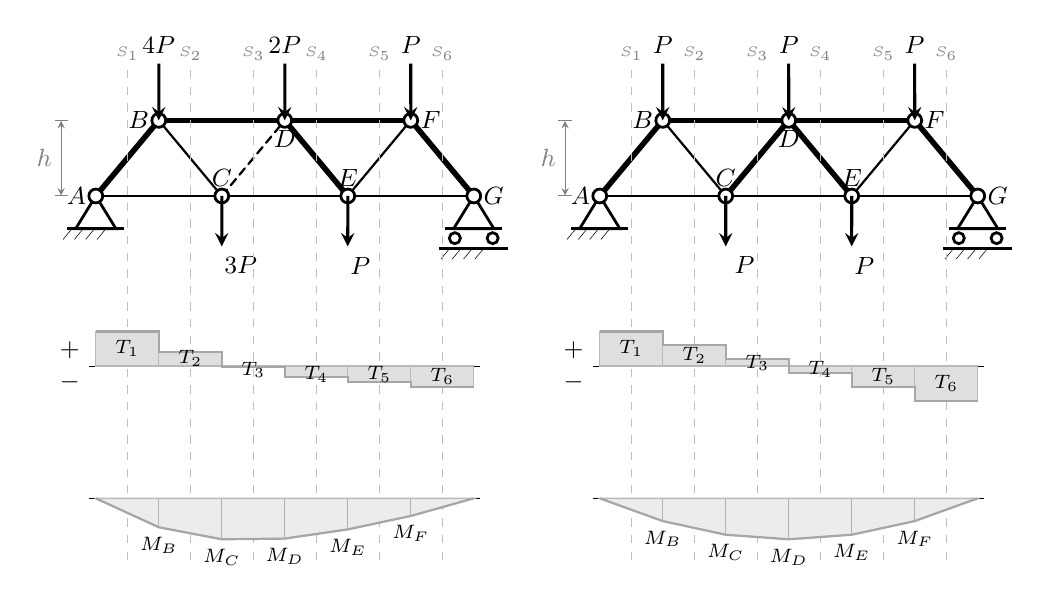
\begin{tikzpicture}[
		scale=0.80,
		comp/.style={line width=2.0pt, line cap=round, line join=round, black},
		tens/.style={line width=0.8pt, line cap=round, line join=round, black},
		zero/.style={line width=0.8pt, line cap=round, line join=round, black,
			dash pattern=on 3pt off 2pt},
		nodo/.style={circle, fill=white, draw=black,
			inner sep=0pt, minimum size=5pt, line width=1.0pt},
		forza/.style={->, >=stealth, line width=1.1pt},
		sez/.style={very thin, gray!50, dashed},
		Tfill/.style={fill=gray!25, draw=gray!55, line width=0.5pt},
		Mfill/.style={fill=gray!15, draw=gray!55, line width=0.5pt},
		Mtick/.style={gray!60, line width=0.5pt},
		]
		
		%%-- COLONNA 1 -------------------------------------------------------
		\coordinate (A)  at (0,0);
		\coordinate (C1) at (2,0);
		\coordinate (E1) at (4,0);
		\coordinate (G)  at (6,0);
		\coordinate (B1) at (1,1.2);
		\coordinate (D1) at (3,1.2);
		\coordinate (F1) at (5,1.2);
		
		%% corrente inferiore: teso (sottile)
		\draw[tens](A)--(C1)--(E1)--(G);
		%% corrente superiore: compresso (spesso)
		\draw[comp](B1)--(D1)--(F1);
		%% diagonali col 1:
		%% AB: salente, T1>0 → compressa
		\draw[comp](A)--(B1);
		%% BC: discendente, T2>0 → tesa
		\draw[tens](B1)--(C1);
		%% CD: salente, T3≈0 → scarica
		\draw[zero](C1)--(D1);
		%% DE: discendente, T4<0 → compressa
		\draw[comp](D1)--(E1);
		%% EF: salente, T5<0 → tesa
		\draw[tens](E1)--(F1);
		%% FG: discendente, T6<0 → compressa
		\draw[comp](F1)--(G);
		
		\foreach \pt in {C1,E1,B1,D1,F1}{\node[nodo]at(\pt){};}
		
		\node[left,  font=\small]at(A)  {$A$};
		\node[left,  font=\small]at(B1) {$B$};
		\node[above, font=\small]at(C1) {$C$};
		\node[below, font=\small]at(D1) {$D$};
		\node[above, font=\small]at(E1) {$E$};
		\node[right, font=\small]at(F1) {$F$};
		\node[right, font=\small]at(G)  {$G$};
		
		\draw[ |<->|,>=stealth,very thin,gray]
		(-0.55,0)--(-0.55,1.2)node[midway,left,font=\small]{$h$};
		
		\draw[forza](1,2.1)--(B1);  \node[above,font=\small]at(1,2.1){$4P$};
		\draw[forza](C1)--(2,-0.8); \node[below,font=\small]at(2.3,-0.8){$3P$};
		\draw[forza](3,2.1)--(D1);  \node[above,font=\small]at(3,2.1){$2P$};
		\draw[forza](E1)--(4,-0.8); \node[above,font=\small]at(4.2,-1.4){$P$};
		\draw[forza](5,2.1)--(F1);  \node[above,font=\small]at(5,2.1){$P$};
		
		\draw[line width=1.0pt](A)--++(-0.32,-0.52)--++(0.64,0)--cycle;
		\draw[line width=1.0pt](-0.45,-0.52)--(0.45,-0.52);
		\foreach \xx in {-0.38,-0.20,-0.02,0.16}
		\draw[very thin](\xx,-0.52)--++(-0.14,-0.17);
		\node[nodo]at(A){};
		
		\draw[line width=1.0pt](G)--++(-0.32,-0.52)--++(0.64,0)--cycle;
		\draw[line width=1.0pt](5.55,-0.52)--(6.45,-0.52);
		\draw[line width=1.0pt](5.70,-0.67)circle(2.5pt);
		\draw[line width=1.0pt](6.30,-0.67)circle(2.5pt);
		\draw[line width=1.0pt](5.45,-0.83)--(6.55,-0.83);
		\foreach \xx in {-0.38,-0.20,-0.02,0.16}
		\draw[very thin](6+\xx,-0.83)--++(-0.14,-0.17);
		\node[nodo]at(G){};
		
		\foreach \xs/\lab in {0.5/$S_1$,1.5/$S_2$,2.5/$S_3$,3.5/$S_4$,4.5/$S_5$,5.5/$S_6$}{
			\draw[sez](\xs,2.0)--(\xs,-5.80);
			\node[above,font=\tiny,gray]at(\xs,2.0){\lab};}
		
		%% taglio col 1
		\draw[thin](-0.1,-2.7)--(6.1,-2.7);
		\node[left,font=\small]at(-0.1,-2.45){$+$};
		\node[left,font=\small]at(-0.1,-2.95){$-$};
		\fill[Tfill](0,-2.7)rectangle(1,-2.15);
		\fill[Tfill](1,-2.7)rectangle(2,-2.472);
		\fill[Tfill](2,-2.713)rectangle(3,-2.7);
		\fill[Tfill](3,-2.875)rectangle(4,-2.7);
		\fill[Tfill](4,-2.955)rectangle(5,-2.7);
		\fill[Tfill](5,-3.036)rectangle(6,-2.7);
		\draw[gray!70,line width=0.8pt]
		(0,-2.15)--(1,-2.15)--(1,-2.472)--(2,-2.472)--
		(2,-2.713)--(3,-2.713)--(3,-2.875)--(4,-2.875)--
		(4,-2.955)--(5,-2.955)--(5,-3.036)--(6,-3.036);
		\node[font=\scriptsize]at(0.5,-2.42){$T_1$};
		\node[font=\scriptsize]at(1.5,-2.58){$T_2$};
		\node[font=\scriptsize]at(2.5,-2.76){$T_3$};
		\node[font=\scriptsize]at(3.5,-2.83){$T_4$};
		\node[font=\scriptsize]at(4.5,-2.83){$T_5$};
		\node[font=\scriptsize]at(5.5,-2.87){$T_6$};
		
		%% momento col 1
		\draw[thin](-0.1,-4.8)--(6.1,-4.8);
		\fill[Mfill]
		(0,-4.8)--(1,-5.259)--(2,-5.450)--(3,-5.439)--
		(4,-5.293)--(5,-5.080)--(6,-4.8)--cycle;
		\draw[gray!70,line width=0.8pt]
		(0,-4.8)--(1,-5.259)--(2,-5.450)--(3,-5.439)--
		(4,-5.293)--(5,-5.080)--(6,-4.8);
		\draw[Mtick](1,-4.8)--(1,-5.259); \node[font=\scriptsize,below]at(1,-5.259){$M_B$};
		\draw[Mtick](2,-4.8)--(2,-5.450); \node[font=\scriptsize,below]at(2,-5.450){$M_C$};
		\draw[Mtick](3,-4.8)--(3,-5.439); \node[font=\scriptsize,below]at(3,-5.439){$M_D$};
		\draw[Mtick](4,-4.8)--(4,-5.293); \node[font=\scriptsize,below]at(4,-5.293){$M_E$};
		\draw[Mtick](5,-4.8)--(5,-5.080); \node[font=\scriptsize,below]at(5,-5.080){$M_F$};
		
		%%-- COLONNA 2 -------------------------------------------------------
		\coordinate (A2) at (8,0);
		\coordinate (C2) at (10,0);
		\coordinate (E2) at (12,0);
		\coordinate (G2) at (14,0);
		\coordinate (B2) at (9,1.2);
		\coordinate (D2) at (11,1.2);
		\coordinate (F2) at (13,1.2);
		
		%% corrente inferiore: teso
		\draw[tens](A2)--(C2)--(E2)--(G2);
		%% corrente superiore: compresso
		\draw[comp](B2)--(D2)--(F2);
		%% diagonali col 2:
		%% AB: salente, T1>0 → compressa
		\draw[comp](A2)--(B2);
		%% BC: discendente, T2>0 → tesa
		\draw[tens](B2)--(C2);
		%% CD: salente, T3>0 → compressa
		\draw[comp](C2)--(D2);
		%% DE: discendente, T4<0 → compressa
		\draw[comp](D2)--(E2);
		%% EF: salente, T5<0 → tesa
		\draw[tens](E2)--(F2);
		%% FG: discendente, T6<0 → compressa
		\draw[comp](F2)--(G2);
		
		\foreach \pt in {C2,E2,B2,D2,F2}{\node[nodo]at(\pt){};}
		
		\node[left, font=\small]at(A2){$A$};
		\node[left, font=\small]at(B2){$B$};
		\node[above,font=\small]at(C2){$C$};
		\node[below,font=\small]at(D2){$D$};
		\node[above,font=\small]at(E2){$E$};
		\node[right,font=\small]at(F2){$F$};
		\node[right,font=\small]at(G2){$G$};
		
		\draw[ |<->|,>=stealth,very thin,gray]
		(7.45,0)--(7.45,1.2)node[midway,left,font=\small]{$h$};
		
		\draw[forza](9,2.1)--(B2);   \node[above,font=\small]at(9,2.1){$P$};
		\draw[forza](C2)--(10,-0.8); \node[below,font=\small]at(10.3,-0.8){$P$};
		\draw[forza](11,2.1)--(D2);  \node[above,font=\small]at(11,2.1){$P$};
		\draw[forza](E2)--(12,-0.8); \node[above,font=\small]at(12.2,-1.4){$P$};
		\draw[forza](13,2.1)--(F2);  \node[above,font=\small]at(13,2.1){$P$};
		
		\draw[line width=1.0pt](A2)--++(-0.32,-0.52)--++(0.64,0)--cycle;
		\draw[line width=1.0pt](7.55,-0.52)--(8.45,-0.52);
		\foreach \xx in {-0.38,-0.20,-0.02,0.16}
		\draw[very thin](8+\xx,-0.52)--++(-0.14,-0.17);
		\node[nodo]at(A2){};
		
		\draw[line width=1.0pt](G2)--++(-0.32,-0.52)--++(0.64,0)--cycle;
		\draw[line width=1.0pt](13.55,-0.52)--(14.45,-0.52);
		\draw[line width=1.0pt](13.70,-0.67)circle(2.5pt);
		\draw[line width=1.0pt](14.30,-0.67)circle(2.5pt);
		\draw[line width=1.0pt](13.45,-0.83)--(14.55,-0.83);
		\foreach \xx in {-0.38,-0.20,-0.02,0.16}
		\draw[very thin](14+\xx,-0.83)--++(-0.14,-0.17);
		\node[nodo]at(G2){};
		
		\foreach \xs/\lab in {8.5/$S_1$,9.5/$S_2$,10.5/$S_3$,11.5/$S_4$,12.5/$S_5$,13.5/$S_6$}{
			\draw[sez](\xs,2.0)--(\xs,-5.80);
			\node[above,font=\tiny,gray]at(\xs,2.0){\lab};}
		
		%% taglio col 2
		\draw[thin](7.9,-2.7)--(14.1,-2.7);
		\node[left,font=\small]at(7.9,-2.45){$+$};
		\node[left,font=\small]at(7.9,-2.95){$-$};
		\fill[Tfill]( 8,-2.7)rectangle( 9,-2.15);
		\fill[Tfill]( 9,-2.7)rectangle(10,-2.37);
		\fill[Tfill](10,-2.7)rectangle(11,-2.59);
		\fill[Tfill](11,-2.81)rectangle(12,-2.7);
		\fill[Tfill](12,-3.03)rectangle(13,-2.7);
		\fill[Tfill](13,-3.25)rectangle(14,-2.7);
		\draw[gray!70,line width=0.8pt]
		(8,-2.15)--(9,-2.15)--(9,-2.37)--(10,-2.37)--
		(10,-2.59)--(11,-2.59)--(11,-2.81)--(12,-2.81)--
		(12,-3.03)--(13,-3.03)--(13,-3.25)--(14,-3.25);
		\node[font=\scriptsize]at( 8.5,-2.42){$T_1$};
		\node[font=\scriptsize]at( 9.5,-2.53){$T_2$};
		\node[font=\scriptsize]at(10.5,-2.65){$T_3$};
		\node[font=\scriptsize]at(11.5,-2.75){$T_4$};
		\node[font=\scriptsize]at(12.5,-2.87){$T_5$};
		\node[font=\scriptsize]at(13.5,-2.98){$T_6$};
		
		%% momento col 2
		\draw[thin](7.9,-4.8)--(14.1,-4.8);
		\fill[Mfill]
		(8,-4.8)--(9,-5.161)--(10,-5.378)--(11,-5.450)--
		(12,-5.378)--(13,-5.161)--(14,-4.8)--cycle;
		\draw[gray!70,line width=0.8pt]
		(8,-4.8)--(9,-5.161)--(10,-5.378)--(11,-5.450)--
		(12,-5.378)--(13,-5.161)--(14,-4.8);
		\draw[Mtick]( 9,-4.8)--( 9,-5.161); \node[font=\scriptsize,below]at( 9,-5.161){$M_B$};
		\draw[Mtick](10,-4.8)--(10,-5.378); \node[font=\scriptsize,below]at(10,-5.378){$M_C$};
		\draw[Mtick](11,-4.8)--(11,-5.450); \node[font=\scriptsize,below]at(11,-5.450){$M_D$};
		\draw[Mtick](12,-4.8)--(12,-5.378); \node[font=\scriptsize,below]at(12,-5.378){$M_E$};
		\draw[Mtick](13,-4.8)--(13,-5.161); \node[font=\scriptsize,below]at(13,-5.161){$M_F$};
		
	\end{tikzpicture}
	\caption{Analogia della trave equivalente per travature
		reticolari piane a correnti paralleli.
		\emph{Colonna sinistra}: carichi asimmetrici
		$4P,\,3P,\,2P,\,P,\,P$ ai nodi $B,C,D,E,F$;
		il diagramma del taglio ha cambio di segno
		tra $T_2$ e $T_3$, e il poligono del momento
		ha massimo in $C$.
		\emph{Colonna destra}: carichi uniformi $P$
		a tutti i nodi interni; il diagramma del taglio
		è antisimmetrico con gradini uguali, e il poligono
		del momento è simmetrico con massimo in $D$.
		I trattini verticali indicano i valori nodali
		$M_B,\ldots,M_F$ del momento flettente equivalente;
		le sezioni $S_1,\ldots,S_6$ mostrano la corrispondenza
		tra taglio nel pannello e aste sezionate:
		lo sforzo nel corrente è proporzionale al momento
		$M/h$, quello nella diagonale al taglio
		$T/\!\cos\alpha$.
		Tratto spesso: asta compressa; tratto sottile:
		asta tesa; tratto tratteggiato: asta scarica
		(colonna sinistra, asta~$CD$).}
	\label{fig:trave_equivalente}
\end{figure}
%%%%%%%%%%%%%%%%%%%%%%%%%%%%%%%%%%%%%%%%%%%%%%%%%%%%%%%%%

\subsubsection{Sforzi nelle aste dei correnti}
\label{subsec:sforzi_correnti}

Si consideri una sezione canonica che taglia un'asta
del corrente superiore, un'asta del corrente inferiore
e un'asta di parete, come illustrato nella
\FIGref{fig:trave_equivalente}. Con correnti orizzontali
ad altezza~$h$, il polo dell'asta di corrente è il
punto~$P$ di intersezione della retta dell'asta di
parete con quella del corrente opposto: per un'asta
di parete verticale (montante), $P$ coincide con il
nodo di intersezione; per un'asta di parete inclinata,
$P$ è il punto proprio o improprio di intersezione.

L'equazione di momento rispetto a~$P$ per la parte
di travatura a sinistra della sezione uguaglia il
momento esterno~$M_\text{eq}(P)$ al momento
interno prodotto dallo sforzo~$N$ nell'asta del
corrente sezionato, con braccio~$h$:
\begin{equation}\label{eq:N_corrente}
	N = \frac{M_\text{eq}(P)}{h}.
\end{equation}
Il segno si determina osservando che il momento
esterno e quello interno devono equilibrarsi: se
procedendo da sinistra il momento esterno in~$P$
è antiorario, lo sforzo~$N$ nell'asta del corrente
deve produrre un momento orario, e viceversa.
Ne segue che il corrente inferiore è teso
($N > 0$) e quello superiore è compresso ($N < 0$)
quando il momento equivalente è positivo,
come nella configurazione ordinaria di trave
appoggiata con carichi verso il basso.

\begin{oss}
	Il vantaggio statico della travatura reticolare
	rispetto a una trave piena di pari ingombro è
	evidente dalla~\EQUref{eq:N_corrente}: lo sforzo
	normale nelle aste di corrente è il momento
	flettente diviso per il braccio $h$. Più alto
	è $h$, minore è $N$ a parità di $M_\text{eq}$.
	Le travature reticolari sfruttano l'altezza
	per ridurre gli sforzi interni, a differenza
	della trave piena che concentra le tensioni
	nelle fibre esterne.
\end{oss}


%............................................................................................................................
\subsubsection{Sforzi nelle aste di parete}
\label{subsec:sforzi_parete}
%............................................................................................................................

Per un'asta di parete inclinata di un angolo $\alpha$
rispetto all'orizzontale, il polo delle altre due
aste sezionate (i due tratti dei correnti) è
un punto improprio se i correnti sono paralleli.
L'equazione di Ritter degenera in un'equazione
di traslazione nella direzione verticale.

La formula che lega $N$ al taglio della trave
equivalente si ricava per \emph{equivalenza}: sia
la risultante verticale delle forze esterne a
sinistra della sezione, sia la componente verticale
degli sforzi nelle aste sezionate rappresentano
la stessa grandezza vista da due prospettive duali.
Con la convenzione di taglio \emph{oraria}
($T_\text{eq} > 0$ se la risultante verticale
delle forze esterne a sinistra è diretta verso
l'alto), la componente verticale delle aste
sezionate deve equilibrare tale risultante verso
il basso sul troncone sinistro. Poiché le aste
dei correnti sono orizzontali e non contribuiscono
alla traslazione verticale, la sola componente
verticale dell'asta di parete deve equilibrare
$T_\text{eq}$:
\begin{equation}\label{eq:N_parete}
	N \sin\alpha = T_\text{eq},
	\qquad \Rightarrow \qquad
	N = \frac{T_\text{eq}}{\sin\alpha},
\end{equation}
Per un montante verticale ($\alpha = 90^\circ$) si ha
$N = T_\text{eq}$ direttamente: il montante è
in trazione quando $T_\text{eq} > 0$ e in
compressione quando $T_\text{eq} < 0$.

In alternativa, lo sforzo nell'asta di parete
si ricava dall'equilibrio orizzontale del troncone
sinistro, osservando che la variazione di sforzo
nei correnti tra i poli $P$ e $Q$ associati
all'asta sezionata deve essere equilibrata dalla
componente orizzontale dell'asta stessa:
\begin{equation}\label{eq:N_parete_DeltaM}
	N \cos\alpha = \frac{\Delta M_{PQ}}{h},
	\qquad \Rightarrow \qquad
	N = \frac{\Delta M_{PQ}}{h \cos\alpha},
\end{equation}
dove $\Delta M_{PQ} = M_\text{eq}(Q) - M_\text{eq}(P)$
è la variazione del momento equivalente tra i due poli.
Le due formule~\eqref{eq:N_parete}
e~\eqref{eq:N_parete_DeltaM} sono coerenti: la
relazione $\Delta M_{PQ} = T_\text{eq} \cdot \overline{PQ}_x$,
dove $(\overline{PQ})_h$ è la proiezione orizzontale
della distanza tra i poli, non è altro che la
definizione di taglio come derivata del momento.



%............................................................................................................................
\subsubsection{Limiti dell'analogia}
\label{subsec:limiti_analogia}
%............................................................................................................................

L'analogia con la trave equivalente si applica
senza modifiche solo quando i carichi e le reazioni
sono \emph{tutti verticali}. In presenza di carichi
orizzontali o di reazioni con componente orizzontale,
l'analogia non è direttamente applicabile per due
ragioni:

\begin{itemize}[noitemsep]
	\item i diagrammi di $T_\text{eq}$ e
	$M_\text{eq}$ della trave equivalente non
	tengono conto delle forze orizzontali;
	\item il momento rispetto a un polo sul corrente
	superiore differisce da quello rispetto a
	un polo sul corrente inferiore, e
	la~\EQUref{eq:N_corrente} non è più univoca.
\end{itemize}

In questi casi il metodo delle sezioni di Ritter
rimane pienamente valido, ma occorre scrivere
esplicitamente le equazioni di equilibrio del
troncone con tutte le componenti di forza, senza
ricorrere ai diagrammi della trave equivalente.
Un'estensione dell'analogia è tuttavia possibile,
anche in presenza di forze orizzontali, costruendo
due distinti poligoni dei momenti --- uno per i nodi
del corrente di intradosso e uno per quelli del
corrente di estradosso. Gli sforzi nei correnti
si ricavano ancora dalla~\EQUref{eq:N_corrente},
leggendo il momento sul poligono corrispondente
al polo dell'asta; gli sforzi nelle aste di parete
dalla~\EQUref{eq:N_parete_DeltaM}, con la variazione
di momento tra i due poligoni nei poli $P$ e $Q$.
Questa estensione rimane valida fintanto che i
correnti sono paralleli. Quando non lo sono ---
come negli archi reticolari --- il braccio~$h$
varia di sezione in sezione e occorre ricorrere
alle equazioni esplicite di equilibrio del troncone.

\subsubsection{Il traliccio di Ritter-M\"{o}rsch come travatura di Warren}

La travatura di Warren\index{travatura!di Warren} costituisce il modello statico
alla base del \emph{traliccio di Ritter-Mörsch}\index{traliccio di Ritter-Morsch@traliccio di Ritter-Mörsch|textbf},
schema interpretativo del comportamento a taglio delle
travi in cemento armato. In questo modello le aste non
hanno tutte la stessa inclinazione: i \emph{puntoni}
--- le bielle di calcestruzzo compresso --- formano un
angolo~$\vartheta$ con l'orizzontale, mentre le
\emph{staffe} --- l'armatura trasversale tesa ---
sono in generale inclinate di un angolo~$\alpha$,
con il caso più comune delle staffe verticali
($\alpha = 90^\circ$) come caso particolare.
La \FIGref{fig:traliccio_Morsch} mostra lo schema
per il caso $\vartheta = 45^\circ$ e $\alpha = 60^\circ$,
con carichi~$P$ applicati ai nodi del corrente superiore.

I quattro elementi del modello corrispondono ad
altrettanti elementi fisici della trave in cemento
armato: il \emph{corrente superiore} rappresenta
la zona compressa del calcestruzzo; il
\emph{corrente inferiore} rappresenta l'armatura
longitudinale tesa; i \emph{puntoni} rappresentano
le bielle di calcestruzzo inclinate che si formano
nell'anima della trave; le \emph{staffe} rappresentano
l'armatura trasversale.

Gli sforzi nei puntoni e nelle staffe si ricavano
direttamente dalle~\EQUref{eq:N_parete}
e~\eqref{eq:N_parete_DeltaM}, con $d$ al posto
di~$h$ per la distanza tra i correnti.
Per le staffe verticali ($\alpha = 90^\circ$) la
formula si riduce a $N_s = T_\text{eq}$: ogni staffa
deve equilibrare da sola il taglio nel pannello
corrispondente. Per i puntoni la formula dà
$N_p = T_\text{eq}/\sin\vartheta$, con segno
negativo (compressione) quando $T_\text{eq} > 0$.


%%%%%%%%%%%%%%%%%%%%%%%%%%%%%%%%%%%%%%%%%%%%%%%%%%%%%%%%%
\begin{figure}[htbp]
	\centering
	\begin{tikzpicture}[
		corrente/.style={line width=2.0pt, line cap=round, line join=round, black},
		puntone/.style={line width=1.8pt, line cap=round, line join=round, black},
		staffa/.style={line width=0.8pt,  line cap=round, line join=round, black},
		nodo/.style={circle, fill=white, draw=black,
			inner sep=0pt, minimum size=5.5pt, line width=1.0pt},
		forza/.style={-{Stealth[length=5pt,width=4pt]}, line width=0.9pt, black},
		quota/.style={ |<->|, >=stealth, very thin, gray!70},
		sez/.style={very thin, gray!40, dashed},
		Tfill/.style={fill=gray!25, draw=gray!55, line width=0.5pt},
		Mfill/.style={fill=gray!15, draw=gray!55, line width=0.5pt},
		lab/.style={font=\small},
		labs/.style={font=\scriptsize},
		]
		
		%% alpha=60: a=cot60=0.5774,  theta=45: b=cot45=1.0,  h=1.40
		\def\h{1.40}
		\pgfmathsetmacro{\ah}{0.5774*\h}
		\pgfmathsetmacro{\bh}{1.0000*\h}
		\pgfmathsetmacro{\abh}{\ah+\bh}
		
		%% ── Nodi ────────────────────────────────────────────────────────
		\coordinate (A) at (0,0);
		\coordinate (B) at (\abh,0);
		\coordinate (C) at (2*\abh,0);
		\coordinate (D) at (3*\abh,0);
		\coordinate (E) at (4*\abh,0);
		\coordinate (F) at (\bh,\h);
		\coordinate (G) at (\ah+2*\bh,\h);
		\coordinate (H) at (3*\ah+2*\bh,\h);
		\coordinate (I) at (4*\ah+3*\bh,\h);
		
		%% ── Correnti ────────────────────────────────────────────────────
		\draw[staffa](A)--(B)--(C)--(D)--(E);
		\draw[corrente](F)--(G)--(H)--(I);
		
		%% ── Puntoni (theta=45, spessi) ──────────────────────────────────
		\draw[puntone](A)--(F);
		\draw[puntone](B)--(G);
		\draw[puntone](H)--(D);
		\draw[puntone](I)--(E);
		
		%% ── Staffe (alpha=60, sottili) ──────────────────────────────────
		\draw[staffa](F)--(B);
		\draw[staffa](G)--(C);
		\draw[staffa](C)--(H);
		\draw[staffa](D)--(I);
		
		%% ── Carichi F (più in alto) ─────────────────────────────────────
		\foreach \nd in {F,G,H,I}{
			\draw[forza]($(\nd)+(0,1.40)$)--($(\nd)+(0,0.70)$);
			\node[above,lab]at($(\nd)+(0,1.50)$){$P$};}
		
		%% ── Cerniera A ──────────────────────────────────────────────────
		\draw[line width=0.9pt](A)--++(-0.26,-0.42)--++(0.52,0)--cycle;
		\draw[line width=0.9pt](-0.36,-0.42)--(0.36,-0.42);
		\foreach \x in {-0.30,-0.15,0.00,0.15,0.30}
		\draw[very thin](\x,-0.42)--++(-.10,-0.13);
		\node[nodo]at(A){};
		
		%% ── Carrello E ──────────────────────────────────────────────────
		\draw[line width=0.9pt](E)--++(-0.26,-0.36)--++(0.52,0)--cycle;
		\draw[line width=0.9pt]($(E)+(-0.36,-0.36)$)--($(E)+(0.36,-0.36)$);
		\draw[line width=0.9pt]($(E)+(-0.18,-0.50)$)circle(2.2pt);
		\draw[line width=0.9pt]($(E)+( 0.18,-0.50)$)circle(2.2pt);
		\draw[line width=0.9pt]($(E)+(-0.36,-0.62)$)--($(E)+(0.36,-0.62)$);
		\foreach \x in {-0.30,-0.15,0.00,0.15,0.30}
		\draw[very thin]($(E)+(\x,-0.62)$)--++(-.10,-0.13);
		\node[nodo]at(E){};
		
		%% ── Nodi interni ────────────────────────────────────────────────
		\foreach \nd in {B,C,D,F,G,H,I}{\node[nodo]at(\nd){};}
		
		%% ── Etichette nodi ──────────────────────────────────────────────
		\node[left,lab]at(A){$A$};
		\node[below,lab]at(B){$B$};
		\node[below,lab]at(C){$C$};
		\node[below,lab]at(D){$D$};
		\node[right,lab]at(E){$E$};
		\node[above,lab]at(F){$F$};
		\node[above,lab]at(G){$G$};
		\node[above,lab]at(H){$H$};
		\node[above,lab]at(I){$I$};
		
		
		%% ── Reazioni 2P in A e E (grigie, coda al nodo, verso l'alto) ──
		\draw[-{Stealth[length=5pt,width=4pt]},gray!60,line width=0.9pt]
		(A)--($(A)+(0,1.40)$);
		\node[above,font=\small,gray!60]at($(A)+(0,1.40)$){$2P$};
		\draw[-{Stealth[length=5pt,width=4pt]},gray!60,line width=0.9pt]
		(E)--($(E)+(0,1.40)$);
		\node[above,font=\small,gray!60]at($(E)+(0,1.40)$){$2P$};
		%% ── Quota h verticale ───────────────────────────────────────────
		\draw[quota](-0.80,0)--(-0.80,\h)node[midway,left,lab]{$h$};
		
		%% ── Angoli theta e alpha ────────────────────────────────────────
		\draw[very thin,gray!60](A)--++(0.55,0);
		\draw[thin,gray!60]($(A)+(0.40,0)$) arc(0:{atan(\h/\bh)}:0.40);
		\node[labs]at($(A)+(0.52,0.16)$){$\vartheta$};
		\draw[very thin,gray!60](F)--++(0.55,0);
		\draw[thin,gray!60]($(F)+(0.40,0)$) arc(0:{-atan(\h/\ah)}:0.40);
		\node[labs]at($(F)+(0.52,-0.22)$){$\alpha$};
		
		%% ── Quote orizzontali (sotto il corrente inferiore) ─────────────
		\def\yq{-0.95}
		%% distanze tra nodi in ordine di ascissa: A,F,B,G,C,H,D,I,E
		%% A->F: bh (=cot theta), F->B: ah (=cot alpha), etc.
		\draw[quota](0,\yq)--(\bh,\yq)
		node[midway,above,labs]{$b$};
		\draw[quota](\bh,\yq)--(\abh,\yq)
		node[midway,above,labs]{$a$};
		\draw[quota](\abh,\yq)--(\ah+2*\bh,\yq)
		node[midway,above,labs]{$b$};
		\draw[quota](\ah+2*\bh,\yq)--(2*\abh,\yq)
		node[midway,above,labs]{$a$};
		\draw[quota](2*\abh,\yq)--(3*\ah+2*\bh,\yq)
		node[midway,above,labs]{$a$};
		\draw[quota](3*\ah+2*\bh,\yq)--(3*\abh,\yq)
		node[midway,above,labs]{$b$};
		\draw[quota](3*\abh,\yq)--(4*\ah+3*\bh,\yq)
		node[midway,above,labs]{$a$};
		\draw[quota](4*\ah+3*\bh,\yq)--(4*\abh,\yq)
		node[midway,above,labs]{$b$};
		
		%% ── Linee di sezione (verticali tratteggiate) ───────────────────
		\foreach \xs in {\bh/2, \bh+\ah/2, \abh+\bh/2,
			\ah+2*\bh+\ah/2, 2*\abh+\ah/2,
			3*\ah+2*\bh+\bh/2, 3*\abh+\ah/2,
			4*\ah+3*\bh+\bh/2}{
			\draw[sez](\xs,1.9)--(\xs,-4.20);}
		
		%% ════════════════════════════════════════════════════════════════
		%% DIAGRAMMA DEL TAGLIO
		%% Shear values: 2F (0 to xF), F (xF to xG), 0 (xG to xH),
		%%               -F (xH to xI), -2F (xI to xE)
		%% Scale: kT=0.50 cm per F
		%% ════════════════════════════════════════════════════════════════
		\def\yT{-2.40}   % zero line del taglio
		\def\kT{0.50}    % cm per unità F
		
		%% zero line
		\draw[line width=1.2pt,black](-0.2,\yT)--(4*\abh+0.2,\yT);
		\node[left,labs]at(-0.2,{\yT+0.25}){$+$};
		\node[left,labs]at(-0.2,{\yT-0.25}){$-$};
		
		%% Pannello 1 (0 a xF): T=+2P (positivo, sopra)
		\fill[Tfill](0,\yT)rectangle(\bh,{\yT+2*\kT});
		%% Pannello 2 (xF a xG): T=+P
		\fill[Tfill](\bh,\yT)rectangle(\ah+2*\bh,{\yT+\kT});
		%% Pannello 3 (xG a xH): T=0
		%% Pannello 4 (xH a xI): T=-P (negativo, sotto)
		\fill[Tfill](3*\ah+2*\bh,{\yT-\kT})rectangle(4*\ah+3*\bh,\yT);
		%% Pannello 5 (xI a xE): T=-2P
		\fill[Tfill](4*\ah+3*\bh,{\yT-2*\kT})rectangle(4*\abh,\yT);
		
		%% profilo a gradini
		\draw[black,line width=0.7pt]
		(0,{\yT+2*\kT})--(\bh,{\yT+2*\kT})--
		(\bh,{\yT+\kT})--(\ah+2*\bh,{\yT+\kT})--
		(\ah+2*\bh,\yT)--(3*\ah+2*\bh,\yT)--
		(3*\ah+2*\bh,{\yT-\kT})--(4*\ah+3*\bh,{\yT-\kT})--
		(4*\ah+3*\bh,{\yT-2*\kT})--(4*\abh,{\yT-2*\kT});
		\draw[black,line width=0.7pt](0,\yT)--(0,{\yT+2*\kT});
		\draw[black,line width=0.7pt](4*\abh,\yT)--(4*\abh,{\yT-2*\kT});
		
		%% etichette
		\node[labs]at({\bh/2},{\yT+\kT}){$2P$};
		\node[labs]at({\bh+\ah/2},{\yT+\kT/2}){$P$};
		\node[labs]at({2*\abh},{\yT+0.15}){$0$};
		\node[labs]at({3*\abh+\ah/2},{\yT-\kT/2}){$P$};
		\node[labs]at({4*\ah+3*\bh+\bh/2},{\yT-\kT}){$2P$};
		
		%% ════════════════════════════════════════════════════════════════
		%% DIAGRAMMA DEL MOMENTO
		%% M values: M_A=0, M_F=2Fbh, M_G=Fh(a+3b), M_H=Fh(a+3b),
		%%           M_I=2Fbh, M_E=0
		%% At B,D: Fh(a+2b)
		%% Scale: kM=0.22 cm per Fh
		%% ════════════════════════════════════════════════════════════════
		\def\yM{-3.80}   % zero line del momento
		\def\kM{0.220}   % cm per Fh
		
		%% valori in cm (moltiplicati per kM, con Fh=1):
		%% M_F = 2bh * kM/h = 2*b*kM = 2*1.0*0.22 = 0.44
		%% M_B = (a+2b)*kM = 2.5774*0.22 = 0.567
		%% M_G = M_H = (a+3b)*kM = 3.5774*0.22 = 0.787
		\pgfmathsetmacro{\mF}{2*1.0*\kM}
		\pgfmathsetmacro{\mB}{(0.5774+2*1.0)*\kM}
		\pgfmathsetmacro{\mG}{(0.5774+3*1.0)*\kM}
		
		%% zero line
		\draw[line width=1.2pt,black](-0.2,\yM)--(4*\abh+0.2,\yM);
		
		%% poligono del momento (positivo verso il basso)
		\fill[Mfill]
		(0,\yM)--
		(\bh,{\yM-\mF})--
		(\abh,{\yM-\mB})--
		(\ah+2*\bh,{\yM-\mG})--
		(3*\ah+2*\bh,{\yM-\mG})--
		(3*\abh,{\yM-\mB})--
		(4*\ah+3*\bh,{\yM-\mF})--
		(4*\abh,\yM)--cycle;
		\draw[black,line width=0.7pt]
		(0,\yM)--
		(\bh,{\yM-\mF})--
		(\abh,{\yM-\mB})--
		(\ah+2*\bh,{\yM-\mG})--
		(3*\ah+2*\bh,{\yM-\mG})--
		(3*\abh,{\yM-\mB})--
		(4*\ah+3*\bh,{\yM-\mF})--
		(4*\abh,\yM);
		
		%% trattini nodali e label
		\draw[gray!50,line width=0.5pt](\bh,\yM)--(\bh,{\yM-\mF});
		\node[labs,below]at(\bh,{\yM-\mF}){$2Pb$};
		\draw[gray!50,line width=0.5pt](\abh,\yM)--(\abh,{\yM-\mB});
		\node[labs,below]at(\abh,{\yM-\mB}){$(a{+}2b)P$};
		\draw[gray!50,line width=0.5pt](\ah+2*\bh,\yM)--(\ah+2*\bh,{\yM-\mG});
		\node[labs,below]at(\ah+2*\bh,{\yM-\mG}){$(a{+}3b)P$};
		%% tetto piatto (da G a H)
		\draw[gray!50,line width=0.5pt](3*\ah+2*\bh,\yM)--(3*\ah+2*\bh,{\yM-\mG});
		\draw[gray!50,line width=0.5pt](3*\abh,\yM)--(3*\abh,{\yM-\mB});
		\draw[gray!50,line width=0.5pt](4*\ah+3*\bh,\yM)--(4*\ah+3*\bh,{\yM-\mF});
		
	\end{tikzpicture}
	\caption{Traliccio di Ritter-M\"{o}rsch con carichi $P$ applicati
		ai nodi del corrente superiore ($F$, $G$, $H$, $I$)
		e reazioni $2P$ agli appoggi $A$ ed $E$.
		Le quote orizzontali indicano le proiezioni delle
		diagonali: $b = \cot\vartheta$ per i puntoni
		(tratto spesso, compressi) e $a = \cot\alpha$
		per le staffe (tratto sottile, tese).
		Il diagramma del taglio è positivo nella metà
		sinistra ($2P$ nel primo pannello, $P$ nel secondo)
		e nullo tra i nodi $G$ e $H$; per antisimmetria
		è negativo nella metà destra.
		Il poligono del momento ha tetto piatto di valore
		$(a+3b)P$ tra $G$ e $H$, dove il taglio è nullo,
		e valori nodali $(a+2b)P$ in $B$ e $D$, $2bP$
		in $F$ e $I$.}
	\label{fig:traliccio_Morsch}
\end{figure}
%%%%%%%%%%%%%%%%%%%%%%%%%%%%%%%%%%%%%%%%%%%%%%%%%%%%%%%%%

Un approccio alternativo, più diretto, consiste
nell'isolare la \emph{maglia elementare} delimitata
da un puntone e da una staffa consecutivi e dai
tratti di corrente compresi tra i loro nodi.
L'equilibrio orizzontale della maglia mostra che
lo sforzo nel corrente superiore varia di
$\Delta N = \Delta M / d$ tra un estremo e l'altro
--- lo stesso squilibrio, di segno opposto, si
riscontra nel corrente inferiore. Questo squilibrio
deve essere equilibrato dalle componenti orizzontali
del puntone e della staffa.

L'equilibrio al nodo comune tra puntone, staffa e
corrente --- dove convergono lo squilibrio~$\Delta N$
(orizzontale), lo sforzo~$N_p$ nel puntone
(inclinato a~$\vartheta$) e lo sforzo~$N_s$ nella
staffa (inclinata a~$\alpha$) --- si riduce alla
chiusura del triangolo delle forze illustrato nella
\FIGref{fig:maglia_Morsch}. 
Il triangolo delle forze ha un angolo al vertice
pari a $\pi - (\vartheta+\alpha)$, opposto al lato
$\Delta N$; poiché $\sin(\pi-(\vartheta+\alpha))
= \sin(\vartheta+\alpha)$, il teorema dei seni dà:
\begin{equation}\label{eq:triangolo_forze}
	\frac{\Delta N}{\sin(\vartheta+\alpha)}
	= \frac{N_p}{\sin\alpha}
	= \frac{N_s}{\sin\vartheta}.
\end{equation}
da cui:
\begin{equation}\label{eq:Np_Ns}
	N_p = \frac{\Delta N\,\sin\alpha}{\sin(\vartheta+\alpha)},
	\qquad
	N_s = \frac{\Delta N\,\sin\vartheta}{\sin(\vartheta+\alpha)}.
\end{equation}
Per staffe verticali ($\alpha = 90^\circ$) si ha
$\sin\alpha = 1$ e $\sin(\vartheta+\alpha) = \cos\vartheta$,
donde:
\begin{equation}\label{eq:Np_Ns_vert}
	N_p = \frac{\Delta N}{\cos\vartheta},
	\qquad
	N_s = \Delta N\,\tan\vartheta.
\end{equation}
La determinazione delle armature necessarie a
resistere a questi sforzi --- e la verifica dei
puntoni di calcestruzzo --- richiedono le proprietà
meccaniche dei materiali e sono oggetto del corso
di \emph{Tecnica delle Costruzioni}.

%%%%%%%%%%%%%%%%%%%%%%%%%%%%%%%%%%%%%%%%%%%%%%%%%%%%%%%%%
\begin{figure}[htbp]
	\centering
	\begin{tikzpicture}[
		corrC/.style={line width=2.0pt, line cap=round, line join=round, black},
		corrT/.style={line width=0.8pt,  line cap=round, line join=round, black},
		punt/.style={line width=1.8pt,  line cap=round, line join=round, black},
		staf/.style={line width=0.8pt,  line cap=round, line join=round, black},
		vett/.style={-{Stealth[length=5pt,width=4pt]}, line width=1.0pt, black},
		forza/.style={-{Stealth[length=5pt,width=4pt]}, line width=0.9pt, black},
		quota/.style={<->, >=stealth, very thin, gray!70},
		lab/.style={font=\small},
		labs/.style={font=\scriptsize},
		]
		
		%% theta=45, alpha=60, d=1.60
		\def\d{1.60}
		\pgfmathsetmacro{\bh}{\d*1.0000}   % d*cot(theta)=1.60
		\pgfmathsetmacro{\ah}{\d*0.5774}   % d*cot(alpha)=0.924
		
		%% Nodi maglia elementare
		\coordinate (I0) at (0,    0);
		\coordinate (I1) at (\bh+\ah, 0);
		\coordinate (S0) at (0,    \d);
		\coordinate (S1) at (\bh+\ah, \d);
		\coordinate (Sp) at (\bh,  \d);   % nodo comune puntone-staffa (in alto)
		
		%%── PANNELLO SINISTRO: maglia elementare ────────────────────────
		%% riquadro grigio chiaro
		\fill[gray!12,rounded corners=2pt]
		(-0.12,-0.18)rectangle(\bh+\ah+0.12,{\d+0.18});
		\draw[gray!40,line width=0.5pt,rounded corners=2pt]
		(-0.12,-0.18)rectangle(\bh+\ah+0.12,{\d+0.18});
		
		%% correnti (con prolungamenti)
		\draw[corrC]($(S0)+(-0.30,0)$)--($(S1)+(0.30,0)$);
		\draw[corrT]($(I0)+(-0.60,0)$)--($(I1)+(0.60,0)$);
		
		%% puntone: I0 -> Sp  (compresso, spesso)
		\draw[punt](I0)--(Sp);
		
		%% staffa: Sp -> I1  (tesa, sottile)
		\draw[staf](Sp)--(I1);
		
		%% nodi
		\foreach \pt in {I0,I1,Sp}{\fill(\pt)circle(2.2pt);}
		
		%% frecce sforzo corrente superiore (compressione: frecce verso l'interno del nodo)
		\draw[forza]($(S0)+(-0.90,0)$)--($(S0)+(-0.35,0)$);
		\draw[forza]($(S1)+(0.90,0)$)--($(S1)+(0.35,0)$);
		\node[above,labs]at($(S0)+(-0.72,0)$){$N$};
		\node[above,labs]at($(S1)+(0.76,0)$){$N{+}\Delta N$};
		
		%% frecce sforzo corrente inferiore (trazione: frecce verso l'esterno del nodo)
		\draw[forza]($(I0)+(-0.35,0)$)--($(I0)+(-0.90,0)$);
		\draw[forza]($(I1)+(0.35,0)$)--($(I1)+(0.90,0)$);
		\node[below,labs]at($(I0)+(-0.72,0)$){$N$};
		\node[below,labs]at($(I1)+(0.76,0)$){$N{+}\Delta N$};
		
		%% quota d
		\draw[quota](-0.95,0)--(-0.95,\d)node[midway,left,lab]{$d$};
		
		%% angolo theta in I0
		\draw[very thin,gray!60](I0)--++(0.50,0);
		\draw[thin,gray!60]($(I0)+(0.38,0)$) arc(0:{atan(\d/\bh)}:0.38);
		\node[labs]at($(I0)+(0.50,0.18)$){$\vartheta$};
		
		%% angolo alpha in Sp
		\draw[very thin,gray!60](Sp)--++(0.50,0);
		\draw[thin,gray!60]($(Sp)+(0.38,0)$) arc(0:{-atan(\d/\ah)}:0.38);
		\node[labs]at($(Sp)+(0.50,-0.22)$){$\alpha$};
		
		%%── PANNELLO DESTRO: triangolo delle forze (equilibrio al nodo Sp) ──
		%% Forze su Sp:
		%%   DeltaN: orizzontale verso SINISTRA (squilibrio compressione corrente sup)
		%%   N_p: verso DESTRA-ALTO a theta (puntone compresso spinge Sp via da I0)
		%%   N_s: verso DESTRA-BASSO a alpha (staffa tesa tira Sp verso I1)
		%%
		%% Poligono chiuso: O --(DeltaN sinistra)--> A --(Np su-destra theta)--> B --(Ns giu-destra alpha)--> O
		
		\def\OX{6.60}
		\def\DN{2.20}   % lunghezza DeltaN
		
		\pgfmathsetmacro{\Np}{\DN*sin(60)/sin(105)}   % N_p = DN*sin(alpha)/sin(theta+alpha)
		\pgfmathsetmacro{\Ns}{\DN*sin(45)/sin(105)}   % N_s = DN*sin(theta)/sin(theta+alpha)
		
		%% Vertici:
		%% O = (OX, 0) — inizio DeltaN / fine N_s
		%% A = (OX-DN, 0) — fine DeltaN / inizio N_p
		%% B = A + Np*(cos45, sin45)
		\pgfmathsetmacro{\Bx}{\OX - \DN + \Np*cos(45)}
		\pgfmathsetmacro{\By}{\Np*sin(45)}
		
		\coordinate (TO) at (\OX, -0.0);
		\coordinate (TA) at (\OX-\DN, -0.0);
		\coordinate (TB) at (\Bx, \By-0.0);
		
		%% lati con frecce
		\draw[vett](TO)--(TA);          % DeltaN verso sinistra
		\draw[vett](TA)--(TB);          % N_p verso destra-alto (theta)
		\draw[vett](TB)--(TO);          % N_s verso destra-basso (alpha)
		
		%% etichette lati
		\node[below,lab]at($(TO)!0.5!(TA)+(0,-0.08)$){$\Delta N$};
		\node[left=0.04,lab]at($(TA)!0.5!(TB)$){$N_p$};
		\node[right=0.04,lab]at($(TB)!0.5!(TO)$){$N_s$};
		
		%% angolo theta in A (tra AO direzione destra e AB direzione su-destra)
		\draw[thin,gray!60]($(TA)+(0.38,0)$) arc(0:45:0.38);
		\node[labs]at($(TA)+(0.50,0.18)$){$\vartheta$};
		
		%% angolo alpha in O (tra OA direzione sinistra e OB direzione su-sinistra)
		%% direzione da O verso B: angolo = atan(By/(Bx-OX))
		\pgfmathsetmacro{\angOB}{atan((\By)/(\Bx-\OX))+180}
		\draw[thin,gray!60]($(TO)+(-0.38,0)$) arc(180:{\angOB}:0.38);
		\node[labs]at($(TO)+(-0.50,0.22)$){$\alpha$};
		
		%% angolo al vertice B
		\node[labs,above=0.06]at(TB){$\pi{-}(\vartheta{+}\alpha)$};
		
	\end{tikzpicture}
	\caption{Maglia elementare del traliccio di Ritter-Mörsch
		e poligono delle forze al nodo del corrente superiore.
		\emph{Pannello sinistro}: la variazione di sforzo
		$\Delta N$ nei correnti --- uguale in valore assoluto
		nel corrente superiore compresso e in quello inferiore
		teso --- deve essere equilibrata dalle componenti
		orizzontali del puntone (tratto spesso, angolo
		$\vartheta$) e della staffa (tratto sottile, angolo
		$\alpha$).
		\emph{Pannello destro}: poligono chiuso delle forze
		al nodo; l'angolo al vertice opposto a $\Delta N$
		vale $\pi - (\vartheta+\alpha)$, donde per il
		teorema dei seni le~\eqref{eq:Np_Ns}.}
	\label{fig:maglia_Morsch}
\end{figure}
%%%%%%%%%%%%%%%%%%%%%%%%%%%%%%%%%%%%%%%%%%%%%%%%%%%%%%%%%


%----------------------------------------------------------------------------------------------------------------------------
\subsection{Aste soggette a carichi generici}
\label{sec:aste_caricate_trasv}
%----------------------------------------------------------------------------------------------------------------------------

L'ipotesi di carichi applicati esclusivamente ai nodi,
posta a fondamento dell'analisi delle travature
reticolari, è talvolta rilassata nella pratica: una
o più aste possono essere soggette a carichi
distribuiti trasversali o longitudinali, a forze
concentrate e a coppie applicate in punti interni.
In tali casi le aste non sono più soggette al solo
sforzo normale, ma presentano anche taglio e momento
flettente.

La strategia d'analisi si articola in \emph{due fasi
	distinte}, fondate sulla seguente osservazione: per
una trave appoggiata a due cerniere, l'equilibrio
è \emph{isostatico} per i carichi trasversali e per
le coppie concentrate --- le reazioni trasversali
alle estremità sono univocamente determinate ---
mentre è \emph{iperstatico} per i carichi
longitudinali, poiché le due reazioni orizzontali
soddisfano una sola equazione di equilibrio,
lasciando indeterminata la distribuzione dello
sforzo normale tra le due estremità. Questa
indeterminazione è risolta dalla prima fase
attraverso l'equilibrio globale della travatura.




%............................................................................................................................
\subsubsection{Prima fase: riduzione a reticolare equivalente}
\label{subsec:fase1_reticolare}
%............................................................................................................................

Ciascuna asta caricata viene isolata e trattata
come una trave appoggiata alle proprie cerniere di
estremità. Si calcolano le \emph{reazioni trasversali}
alle estremità risolvendo l'equilibrio trasversale
dell'asta isolata sotto i carichi trasversali e le
coppie assegnati: il problema è isostatico e le
reazioni sono univocamente determinate. Le
\emph{reazioni longitudinali} restano invece
indeterminate a questo livello.

Le reazioni trasversali così calcolate vengono
applicate ai nodi di estremità come forze concentrate
aggiuntive, con verso opposto a quello delle reazioni
sull'asta (per il principio di azione e reazione).
In questo modo il sistema si riconduce a una
\emph{travatura reticolare equivalente} in cui tutti
i carichi sono nodali: i carichi originariamente
applicati ai nodi, aumentati delle reazioni
trasversali di estremità delle aste caricate.

La travatura equivalente si analizza con i metodi
ordinari --- metodo dei nodi o metodo di Ritter ---
e fornisce lo sforzo normale $N_e$ all'estremità
destra di ciascuna asta caricata. In presenza di
carichi longitudinali distribuiti $p(z)$ o di
forze concentrate longitudinali in punti interni,
lo sforzo normale non è costante lungo l'asta:
esso varia con legge determinata dall'equilibrio
locale, e la reazione longitudinale all'estremità
sinistra vale
\begin{equation}\label{eq:reazione_long_sinistra}
	N(0) = N_e + \int_0^\ell p(z^e)\,\mathrm{d}z^e
	+ \sum_k Z_k,
\end{equation}
dove $Z_k$ sono le componenti longitudinali
delle forze concentrate applicate in punti interni.
In assenza di carichi longitudinali, $N(z^e) = N_e$
è costante e le reazioni longitudinali alle due
estremità sono uguali in modulo.

La \FIGref{fig:asta_caricata} illustra la procedura
per una capriata con l'asta $AC$ soggetta al carico
trasversale $p$ e al carico longitudinale $q$.
Il pannello~(a) mostra i carichi applicati all'asta
nel contesto della struttura globale; il pannello~(b)
mostra l'asta isolata nel proprio riferimento locale,
con le reazioni trasversali $R_A^\perp$ e $R_C^\perp$
e le reazioni longitudinali $N(0)$ e $N_e$ alle
cerniere di estremità. Tutte queste reazioni,
cambiate di segno per il principio di azione e
reazione, vengono applicate come forze nodali
equivalenti ai nodi $A$ e $C$ della travatura
reticolare equivalente, la cui soluzione fornisce
$N_e$ e quindi $N(0)$ tramite
la~\EQUref{eq:reazione_long_sinistra}.



%%%%%%%%%%%%%%%%%%%%%%%%%%%%%%%%%%%%%%%%%%%
\begin{figure}[htbp]
	\centering
	\resizebox{\textwidth}{!}{%
		\begin{tikzpicture}[
			asta/.style={line width=1.5pt, line cap=round,
				line join=round},
			nodo/.style={circle, fill=white, draw=black,
				inner sep=0pt, minimum size=6pt,
				line width=1.2pt},
			forza/.style={->, >=stealth, line width=1.0pt,
				gray!60!black},
			]
			
			%============================================================
			% PANNELLO A — schema di carico (sinistra)
			%============================================================
			\begin{scope}[shift={(0,0)}, scale=0.62]
				
				\coordinate (A) at (0,0);
				\coordinate (B) at (8,0);
				\coordinate (C) at (4,3);
				\coordinate (D) at (4,0);
				
				%% carico trasversale p (perpendicolare ad AC, sopra)
				\draw[gray!60!black, thin]
				($(A)+0.9*(-0.6,0.8)$)--($(C)+0.9*(-0.6,0.8)$);
				\draw[gray!60!black, thin]
				($(A)+0.25*(-0.6,0.8)$)--($(C)+0.25*(-0.6,0.8)$);
				\foreach \t in {0.0, 0.2, 0.4, 0.6, 0.8, 1.0}{
					\draw[forza]
					($(A)!{\t}!(C)+0.9*(-0.6,0.8)$)
					--($(A)!{\t}!(C)+0.25*(-0.6,0.8)$);
				}
				\node[above left, font=\small, gray!60!black]
				at ($(A)!0.5!(C)+1.0*(-0.6,0.8)$){$p$};
				
				%% carico longitudinale q (radente sotto AC, da A verso C)
				\foreach \t in {0.05, 0.28, 0.51, 0.74}{
					\draw[forza]
					($(A)!{\t}!(C)+0.3*(0.6,-0.8)$)
					--($(A)!{\t+0.18}!(C)+0.3*(0.6,-0.8)$);
				}
				\node[below right, font=\small, gray!60!black]
				at ($(A)!0.5!(C)+0.4*(0.6,-0.8)$){$q$};
				
				%% aste
				\draw[asta] (A)--(C);
				\draw[asta] (C)--(B);
				\draw[asta] (A)--(D);
				\draw[asta] (D)--(B);
				\draw[asta] (C)--(D);
				
				%% cerniera A
				\draw[line width=1.2pt]
				(A)--++(-0.4,-0.65)--++(0.8,0)--cycle;
				\draw[line width=1.2pt](-0.55,-0.65)--(0.55,-0.65);
				\foreach \x in {-0.45,-0.25,-0.05,0.15,0.35}
				\draw[thin](\x,-0.65)--++(-.18,-.22);
				
				%% carrello B
				\draw[line width=1.2pt]
				(B)--++(-0.4,-0.50)--++(0.8,0)--cycle;
				\draw[line width=1.2pt]
				($(B)+(-0.50,-0.50)$)--($(B)+(0.50,-0.50)$);
				\draw[line width=1.2pt]($(B)+(-0.25,-0.65)$) circle(3.5pt);
				\draw[line width=1.2pt]($(B)+( 0.25,-0.65)$) circle(3.5pt);
				\draw[line width=1.2pt]
				($(B)+(-0.55,-0.82)$)--($(B)+(0.55,-0.82)$);
				\foreach \x in {-0.45,-0.25,-0.05,0.15,0.35}
				\draw[thin]($(B)+(\x,-0.82)$)--++(-.18,-.22);
				
				%% nodi
				\node[nodo] at (A){};  \node[nodo] at (B){};
				\node[nodo] at (C){};  \node[nodo] at (D){};
				
				%% etichette nodi
				\node[left,  font=\normalsize] at (A){$A$};
				\node[right, font=\normalsize] at (B){$B$};
				\node[right, font=\normalsize] at (C){$C$};
				\node[below, font=\normalsize] at (D){$D$};
				
				%% etichetta pannello
				\node[font=\small] at (4,-1.5) {$(a)$};
				
			\end{scope}
			
			%============================================================
			% PANNELLO B — asta isolata (destra)
			%============================================================
			\begin{scope}[shift={(7,0)}, scale=0.62]
				
				%% asta isolata orizzontale nel rif. locale
				\draw[asta] (0,0)--(8,0);
				
				%% tratteggio sotto l'asta (riferimento locale)
				\draw[thin, dashed] (0,-0.3)--(8,-0.3);
				
				%% carico trasversale p
				\draw[gray!60!black, thin] (0,2.5)--(8,2.5);
				\draw[black, thin] (0,1.85)--(8,1.85);
				\foreach \x in {0,1,2,3,4,5,6,7,8}{
					\draw[forza] (\x,2.5)--(\x,1.85);
				}
				\node[above, font=\small, gray!60!black] at (4,2.5){$p$};
				
				%% carico longitudinale q (radente, da A verso C)
				\foreach \t in {0.5, 2.0, 3.5, 5.0, 6.5}{
					\draw[forza] (\t,0.4)--(\t+0.8,0.4);
				}
				\node[above, font=\small, gray!60!black] at (4,0.4){$q$};
				
				%% sforzo normale Ne (esce da C verso destra)
				\draw[->, >=stealth, line width=1.5pt, black]
				(8,0)--(9.5,0);
				\node[above, font=\normalsize] at (9.5,0){$N_e$};
				
				%% sforzo normale N(0) (esce da A verso sinistra)
				\draw[->, >=stealth, line width=1.5pt, black]
				(0,0)--(-1.5,0);
				\node[above, font=\normalsize] at (-1.5,0){$N(0)$};
				
				%% reazioni trasversali (coda in A e C, verso l'alto)
				\draw[->, >=stealth, gray!60!black, line width=1.0pt]
				(0,0)--(0,1.35);
				\node[left, font=\small] at (0,1.2){$R_A^\perp$};
				\draw[->, >=stealth, gray!60!black, line width=1.0pt]
				(8,0)--(8,1.35);
				\node[right, font=\small] at (8,1.2){$R_C^\perp$};
				
				%% nodi
				\node[nodo] at (0,0){};
				\node[nodo] at (8,0){};
				
				%% etichette nodi
				\node[below left,  font=\normalsize] at (0,0){$A$};
				\node[below right, font=\normalsize] at (8,0){$C$};
				
				%% etichetta pannello
				\node[font=\small] at (4,-1.5) {$(b)$};
				
			\end{scope}
			
		\end{tikzpicture}
	}% fine resizebox
	\caption{Asta reticolare $AC$ soggetta a carichi generici.
		\emph{(a)}: schema strutturale della capriata con
		carico trasversale $p$ (perpendicolare ad $AC$,
		sopra l'asta) e carico longitudinale $q$
		(radente ad $AC$ da $A$ verso $C$).
		\emph{(b)}: asta $AC$ isolata nel riferimento locale
		con $z^e$ diretto da $A$ verso $C$;
		$N_e$ e $N(0)$ sono gli sforzi normali uscenti
		dalle due estremità; $R_A^\perp$ e $R_C^\perp$
		sono le reazioni trasversali alle cerniere.}
	\label{fig:asta_caricata}
\end{figure}
%%%%%%%%%%%%%%%%%%%%%%%%%%%%%%%%%%%%%%%%%%%

%............................................................................................................................
\subsubsection{Seconda fase: analisi locale dell'asta}
\label{subsec:fase2_locale}
%............................................................................................................................

Una volta noto lo sforzo normale $N$ dalla prima
fase, si analizza l'asta separatamente come
\emph{trave appoggiata} soggetta simultaneamente
a tutti i carichi applicati: distribuiti trasversali
e longitudinali, forze concentrate e coppie in
punti interni, e le forze assiali $N$ alle estremità.

Si calcolano i diagrammi di $N(z)$, $T(z)$ e $M(z)$
lungo l'asta con i metodi ordinari della trave
singola (\CAPref{cap:Diagrammi_CS}). Le condizioni
al contorno sono:
\begin{itemize}[noitemsep]
	\item momento nullo alle cerniere di estremità:
	$M(0) = M(\ell) = 0$;
	\item reazioni trasversali alle estremità
	determinate nella prima fase;
	\item sforzo normale $N(z^e)$ variabile lungo l'asta
	in presenza di carichi longitudinali distribuiti
	o concentrati, con $N_e$ noto dalla prima fase
	come condizione al contorno all'estremità destra
	e $N(0)$ determinato dall'equilibrio locale;
	in assenza di carichi longitudinali, $N(z^e) = N_e$
	è uniforme.
\end{itemize}


\begin{oss}
	Il disaccoppiamento tra la prima e la seconda
	fase è esatto per una ragione puramente statica:
	le reazioni trasversali alle cerniere di estremità
	dipendono esclusivamente dai carichi applicati
	all'asta e non da $N_e$, mentre le reazioni
	longitudinali dipendono da $N_e$ ma non dai
	carichi trasversali. Le due fasi non sono
	intercambiabili: la prima deve precedere la
	seconda perché $N_e$ --- determinato dalla
	soluzione della travatura equivalente --- è
	un dato necessario per la costruzione dei
	diagrammi $N(z^e)$, $T(z^e)$ e $M(z^e)$
	nella seconda fase.
\end{oss}

\begin{oss}
	Le coppie concentrate applicate in punti interni
	all'asta non si trasmettono alle cerniere di
	estremità come momenti --- il momento è nullo
	per definizione alle cerniere --- ma la loro
	presenza si risente ai nodi attraverso le
	reazioni trasversali di estremità che le
	equilibrano. Queste reazioni, calcolate già
	nella prima fase trattando l'asta come trave
	appoggiata, vengono applicate ai nodi della
	travatura equivalente esattamente come quelle
	prodotte dai carichi distribuiti trasversali.
	Nella seconda fase la coppia produce una
	discontinuità nel diagramma del momento nel
	punto di applicazione, senza alcun effetto
	sul diagramma del taglio.
\end{oss}

%............................................................................................................................
\subsubsection{Validità della separazione in due fasi}
\label{subsec:validita_due_fasi}
%............................................................................................................................

La separazione in due fasi è \emph{esatta} perché
non modifica la struttura delle incognite del
problema reticolare. I carichi applicati all'asta
--- trasversali e longitudinali --- vengono
integralmente trasferiti ai nodi nella prima fase:
le reazioni trasversali di estremità equilibrano
i carichi trasversali e le coppie, mentre la
risultante dei carichi longitudinali è riportata
al nodo sinistro come forza nota. L'unica incognita
che rimane è $N_e$ all'estremità destra, determinata
dalla soluzione della travatura equivalente con i
metodi ordinari. La seconda fase risolve poi
l'equilibrio locale dell'asta con $N_e$ noto.


\begin{esempio}[Travatura a correnti paralleli con carico distribuito]
	Si consideri una travatura reticolare a correnti
	paralleli di luce $\ell = 4d$ e altezza $h$, con
	$n_n = 6$ nodi, $n_a = 9$ aste e vincolata con
	una cerniera nel nodo $A$ e un carrello verticale
	nel nodo $B$. I nodi del corrente superiore sono
	$C$, $E$, $F$ e quelli del corrente inferiore
	$A$, $D$, $B$, con passo $d$. Le aste di parete
	sono le diagonali $CD$, $DF$ e il montante $DE$
	(\FIGref{fig:travatura_correnti}).
	Un carico distribuito verticale $q$ (verso il
	basso) agisce sull'asta del corrente superiore
	$CF$ di lunghezza $2d$.
	Si determinino: le reazioni vincolari, gli sforzi
	nelle aste del corrente superiore e inferiore
	nel pannello centrale e lo sforzo nella diagonale,
	usando il metodo di Ritter e l'analogia con la
	trave equivalente.
	
	\begin{svolgimento}
		%%%%%%%%%%%%%%%%%%%%%%%%%%%%%%%%%%%%%%%%%%%
		\begin{figure}[htbp]
			\centering
			\begin{tikzpicture}[
				>=stealth,
				line cap=round,
				line join=round,
				]
				
				%------------------------------------------------------------
				% VINCOLO DI CERNIERA IN A
				%------------------------------------------------------------
				\draw[line width=1pt] (0,0)--(-0.4,-0.6)--(0.4,-0.6)--cycle;
				\draw[line width=0.8pt] (-0.50,-0.60)--(0.50,-0.60);
				\foreach \xi in {-0.40,-0.20,0.00,0.20}{
					\draw[thin] (\xi,-0.60)--(\xi-0.15,-0.85);
				}
				
				%------------------------------------------------------------
				% VINCOLO DI CARRELLO IN B
				%------------------------------------------------------------
				\draw[line width=1pt] (8,0)--(7.60,-0.60)--(8.40,-0.60)--cycle;
				\draw[line width=0.8pt] (7.50,-0.60)--(8.50,-0.60);
				\draw[line width=0.8pt] (7.75,-0.69) circle(0.09);
				\draw[line width=0.8pt] (8.25,-0.69) circle(0.09);
				\draw[line width=0.8pt] (7.50,-0.78)--(8.50,-0.78);
				\foreach \xi in {7.50,7.70,7.90,8.10,8.30}{
					\draw[thin] (\xi,-0.78)--(\xi-0.15,-1.03);
				}
				
				
				%------------------------------------------------------------
				% TRUSS
				%------------------------------------------------------------
				\draw[line width=1.5pt] (0,0)--(4,0)--(8,0);
				\draw[line width=1.5pt] (2,1.4)--(4,1.4)--(6,1.4);
				\draw[line width=1pt] (0,0)--(2,1.4);
				\draw[line width=1pt] (2,1.4)--(4,0);
				\draw[line width=1pt] (4,0)--(4,1.4);
				\draw[line width=1pt] (4,0)--(6,1.4);
				\draw[line width=1pt] (6,1.4)--(8,0);
				
				\foreach \x/\y in {0/0, 4/0, 8/0, 2/1.4, 4/1.4, 6/1.4}{
					\fill[white] (\x,\y) circle(3pt);
					\draw        (\x,\y) circle(3pt);
				}
				
				\node[above left,  font=\small] at (0,0)   {$A$};
				\node[below,       font=\small] at (4,0)   {$D$};
				\node[above right, font=\small] at (8,0)   {$B$};
				\node[above left,  font=\small] at (2,1.4) {$C$};
				\node[above right,       font=\small] at (4,1.4) {$E$};
				\node[above right, font=\small] at (6,1.4) {$F$};
				
				%------------------------------------------------------------
				% CARICO DISTRIBUITO
				%------------------------------------------------------------
				\draw (2,2.3)--(6,2.3);
				\foreach \x in {2, 2.67, 3.33, 4.00, 4.67, 5.33, 6.00}{
					\draw[->] (\x,2.3)--(\x,1.90);
				}
				\draw (2,1.90)--(6,1.90);
				\node[left, font=\small] at (2,2.10) {$q$};
				%		\draw (2,2.3)--(6,2.3);
				%		\foreach \x in {2, 2.67, 3.33, 4.00, 4.67, 5.33, 6.00}{
					%			\draw[->] (\x,2.3)--(\x,1.50);
					%		}
				%		\node[above, font=\small] at (4,2.3) {$q$};
				%		\draw[<->,thin] (2,1.95)--(6,1.95);
				%\node[above, font=\scriptsize] at (4,1.95) {$2d$};
				
				%------------------------------------------------------------
				% SEZIONE DI RITTER
				%------------------------------------------------------------
				\draw[dashed, line width=0.8pt]
				(5.3,1.9) .. controls (5.7,0.7) .. (5.3,-0.2);
				\node[right, font=\scriptsize] at (5.6,0.5) {sez.~Ritter};
				
				%------------------------------------------------------------
				% QUOTATURA ALTEZZA h
				%------------------------------------------------------------
				\draw[|<->|,thin] (-0.6,0)--(-0.6,1.4);
				\node[left, font=\small] at (-0.6,0.7) {$h$};
				\draw[thin] (-0.75,0)--(-0.45,0);
				\draw[thin] (-0.75,1.4)--(-0.45,1.4);
				
				%------------------------------------------------------------
				% QUOTATURA CON CAMPI d
				%------------------------------------------------------------
				\foreach \xa/\xb in {0/2, 2/4, 4/6, 6/8}{
					\draw[<->,thin] (\xa,-1.25)--(\xb,-1.25);
				}
				\foreach \x in {0,2,4,6,8}{
					\draw[thin] (\x,-1.17)--(\x,-1.33);
				}
				\node[above, font=\scriptsize] at (1,-1.25) {$d$};
				\node[above, font=\scriptsize] at (3,-1.25) {$d$};
				\node[above, font=\scriptsize] at (5,-1.25) {$d$};
				\node[above, font=\scriptsize] at (7,-1.25) {$d$};
				%\node[below=0.28cm, font=\small] at (4,-1.25) {$L=4d$};
				
				%------------------------------------------------------------
				% TRAVE EQUIVALENTE
				%------------------------------------------------------------
				%\node[font=\small, gray] at (4,-2.1) {trave equivalente};
				\draw[line width=1.5pt] (0,-2.4)--(8,-2.4);
				%\foreach \x in {0,2,4,6,8}{
					%	\fill[white] (\x,-2.4) circle(2.5pt);
					%	\draw        (\x,-2.4) circle(2.5pt);
					%}
				% carichi nodali equivalenti
				\draw[->] (2,-1.95)--(2,-2.35);
				\node[left, font=\small] at (2,-1.95) {$\tfrac{qd}{2}$};
				\draw[->] (4,-1.75)--(4,-2.35);
				\node[right, font=\small] at (4,-1.75) {$qd$};
				\draw[->] (6,-1.95)--(6,-2.35);
				\node[right, font=\small] at (6,-1.95) {$\tfrac{qd}{2}$};
				% reazioni
				\draw[->] (0,-2.85)--(0,-2.45);
				\node[left, font=\small] at (0,-2.85) {$qd$};
				\draw[->] (8,-2.85)--(8,-2.45);
				\node[right, font=\small] at (8,-2.85) {$qd$};
				
				%------------------------------------------------------------
				% DIAGRAMMA M_eq (positivo verso il basso)
				%------------------------------------------------------------
				\fill[gray!15]
				(0,-2.4)--(2,-3.65)--(4,-4.15)--(6,-3.65)--(8,-2.4)--cycle;
				\draw (0,-2.4)--(2,-3.65)--(4,-4.15)--(6,-3.65)--(8,-2.4);
				\draw[dashed,thin] (2,-2.4)--(2,-3.65);
				\draw[dashed,thin] (4,-2.4)--(4,-4.15);
				\draw[dashed,thin] (6,-2.4)--(6,-3.65);
				\node[left,  font=\small] at (2.7,-3.15) {$qd^2$};
				\node[below, font=\small] at (4.5,-2.85) {$\tfrac{3}{2}qd^2$};
				\node[right, font=\small] at (6,-3.15) {$qd^2$};
				\node[right, font=\small] at (8.2,-3.27) {$M_{\!\text{eq}}$};
				
				%------------------------------------------------------------
				% DIAGRAMMA T_eq
				%------------------------------------------------------------
				
				% +qd (A → C)
				\fill[gray!15] (0,-4.95)--(0,-4.45)--(2,-4.45)--(2,-4.95)--cycle;
				\draw (0,-4.95)--(0,-4.45)--(2,-4.45)--(2,-4.95);
				\node[above, font=\small] at (1,-4.45) {$+qd$};
				% +qd/2 (C → E)
				\fill[gray!15] (2,-4.95)--(2,-4.70)--(4,-4.70)--(4,-4.95)--cycle;
				\draw (2,-4.95)--(2,-4.70)--(4,-4.70)--(4,-4.95);
				\node[above, font=\scriptsize] at (3,-4.70) {$+\tfrac{qd}{2}$};
				% −qd/2 (E → F)
				\fill[gray!15] (4,-4.95)--(4,-5.20)--(6,-5.20)--(6,-4.95)--cycle;
				\draw (4,-4.95)--(4,-5.20)--(6,-5.20)--(6,-4.95);
				\node[below, font=\scriptsize] at (5,-5.20) {$-\tfrac{qd}{2}$};
				% −qd (F → B)
				\fill[gray!15] (6,-4.95)--(6,-5.45)--(8,-5.45)--(8,-4.95)--cycle;
				\draw (6,-4.95)--(6,-5.45)--(8,-5.45)--(8,-4.95);
				\node[below, font=\small] at (7,-5.45) {$-qd$};
				\node[right, font=\small] at (8.2,-4.95) {$T_{\!\text{eq}}$};
				% linea di riferimento del diagramma
				\draw[line width=0.7pt, black] (0,-4.95)--(8,-4.95);
				
				
				
			\end{tikzpicture}
			\caption{Travatura a correnti paralleli con carico
				distribuito sul corrente superiore. In alto:
				schema strutturale con sezione di Ritter
				tratteggiata nel pannello centrale. In basso:
				trave equivalente con diagrammi $M_\text{eq}$
				e $T_\text{eq}$.}
			\label{fig:travatura_correnti}
		\end{figure}
		%%%%%%%%%%%%%%%%%%%%%%%%%%%%%%%%%%%%%%%%%%%
		
		
		\noindent\textbf{Verifica della classificazione.}
		\[
		\nu = 2 \times 6 - 9 - 3 = 0. \quad\checkmark
		\]
		
		\noindent\textbf{Riduzione a reticolare equivalente.}
		Il carico distribuito $q$ agisce sull'asta $CF$ di
		lunghezza $2d$, che comprende due aste distinte:
		$CE$ e $EF$, ciascuna di lunghezza $d$.
		Si isola ciascuna asta come trave appoggiata alle
		proprie cerniere di estremità e si calcolano le
		reazioni trasversali per simmetria:
		\[
		R_C = R_E^{(CE)} = \frac{qd}{2}
		\quad \text{(asta } CE\text{)},
		\qquad
		R_E^{(EF)} = R_F = \frac{qd}{2}
		\quad \text{(asta } EF\text{)}.
		\]
		Nel nodo $E$ confluiscono i contributi delle due aste,
		per cui il carico nodale equivalente risulta doppio:
		\[
		F_C = \frac{qd}{2} \downarrow, \qquad
		F_E = \frac{qd}{2} + \frac{qd}{2} = qd \downarrow, \qquad
		F_F = \frac{qd}{2} \downarrow.
		\]
		
		\noindent\textbf{Reazioni vincolari.}
		Per simmetria del carico equivalente rispetto alla
		mezzeria:
		\[
		Y_A = Y_B = \frac{2qd}{2} = qd
		\quad\text{(verso l'alto)}, \qquad X_A = 0.
		\]
		
		\noindent\textbf{Trave equivalente.}
		La trave equivalente è una trave appoggiata in $A$
		e $B$, con asse coincidente con il corrente inferiore,
		luce $4d$ e ascissa $x$ misurata da $A$ verso $B$.
		È soggetta a tre forze concentrate verso il basso:
		$qd/2$ in $x=d$ (sotto il nodo $C$),
		$qd$ in $x=2d$ (sotto il nodo $E$) e
		$qd/2$ in $x=3d$ (sotto il nodo $F$).
		I diagrammi sono:
		\[
		M_\text{eq}(x) = \begin{cases}
			qd \, x & 0 \leq x \leq d, \\
			qd \, x - \dfrac{qd}{2}(x-d) & d < x \leq 2d, \\
			qd(4d-x) - \dfrac{qd}{2}(4d-x-d) & 2d < x \leq 3d, \\
			qd(4d - x) & 3d < x \leq 4d,
		\end{cases}
		\]
		\[
		T_\text{eq}(x) = \begin{cases}
			+qd & 0 \leq x < d, \\
			+\dfrac{qd}{2} & d < x < 2d, \\
			-\dfrac{qd}{2} & 2d < x < 3d, \\
			-qd & 3d < x \leq 4d.
		\end{cases}
		\]
		Il momento flettente raggiunge il valore massimo
		$\tfrac{3}{2}qd^2$ in $x = 2d$, sezione verticale
		passante per il nodo  $D$ della travatura e polo
		di Ritter dell'asta del corrente superiore  $EF$;
		il taglio è costante a tratti e cambia segno
		in corrispondenza delle sezioni di applicazione
		dei carichi nodali equivalenti.
		
		\noindent\textbf{Sforzi nei correnti (analogia).}
		Nel pannello di destra si taglia con la sezione
		di Ritter che attraversa il corrente superiore
		$EF$, la diagonale $DF$ e il corrente inferiore
		$DB$. Si considera l'equilibrio del troncone
		sinistro. Gli sforzi nelle aste tagliate sono
		positivi se escono dal troncone (trazione) e
		negativi se vi rientrano (compressione).
		Per l'equilibrio alla rotazione del troncone
		sinistro rispetto a un polo, il momento delle
		forze esterne (reazioni e carichi nodali) deve
		essere uguale e opposto al momento prodotto dagli
		sforzi nelle aste tagliate. Poiché nel polo
		convergono due delle tre aste tagliate, il loro
		contributo al momento è nullo e l'equazione di
		equilibrio coinvolge la sola asta di cui si cerca
		lo sforzo. Il segno di quest'ultimo è determinato
		dal confronto tra il verso del momento esterno
		e il verso del momento prodotto dall'asta
		nell'ipotesi di trazione ($N > 0$, forza uscente
		dal troncone).
		
		\medskip
		\noindent\textit{Corrente superiore $N_{EF}$},
		polo $D$ ($x=2d$), braccio $h$.
		Il momento esterno in $D$ è orario:
		$M_\text{eq}(2d) = \tfrac{3}{2}qd^2 > 0$.
		$N_{EF}$ produce momento orario in $D$ se è
		positivo (trazione): per equilibrare il momento
		esterno deve quindi essere negativo (compressione):
		\[
		N_{EF} = -\frac{M_\text{eq}(2d)}{h}
		= -\frac{3qd^2}{2h}
		\quad\text{(compressione)}.
		\]
		
		\noindent\textit{Corrente inferiore $N_{DB}$},
		polo $F$ ($x=3d$), braccio $h$.
		Il momento esterno in $F$ è orario:
		$M_\text{eq}(3d) = qd^2 > 0$.
		$N_{DB}$ produce momento antiorario in $F$ se è
		positivo (trazione): il segno positivo equilibra
		il momento esterno orario:
		\[
		N_{DB} = +\frac{M_\text{eq}(3d)}{h}
		= +\frac{qd^2}{h}
		\quad\text{(trazione)}.
		\]
		
		\noindent\textbf{Sforzo nella diagonale $N_{DF}$.}
		Nel pannello di destra il taglio della trave
		equivalente vale $T_\text{eq} = -qd/2$: la
		risultante verticale delle forze esterne sul
		troncone destro è diretta verso l'alto con
		intensità $qd/2$. La diagonale $DF$ è l'unica
		asta tagliata con componente verticale non nulla
		(le aste $EF$ e $DB$ sono orizzontali); per
		equilibrare la risultante verticale essa deve
		fornire una componente verticale verso il basso,
		il che corrisponde a compressione. Indicato con
		$\alpha$ l'angolo della diagonale rispetto
		all'orizzontale:
		\[
		N_{DF} = \frac{T_\text{eq}}{\sin\alpha}
		= \frac{qd/2}{\sin\alpha}
		\quad\text{(trazione)}.
		\]
		
		\noindent\textbf{Sforzo nel montante $N_{DE}$.}
		Il nodo $E$ è il più semplice da analizzare:
		vi convergono le sole aste orizzontali $CE$ ed
		$EF$ e il montante verticale $DE$. Le componenti
		verticali di $N_{CE}$ e $N_{EF}$ sono nulle;
		l'equilibrio verticale del nodo $E$ sotto il
		carico nodale equivalente $qd$ dà quindi:
		\[
		N_{DE} - qd = 0 \implies N_{DE} = -qd
		\quad\text{(compressione)}.
		\]
		Il montante scarica direttamente al corrente
		inferiore il carico nodale applicato in $E$.
		
		\medskip
		\noindent\textbf{Considerazioni di simmetria.}
		Il carico equivalente --- $qd/2$ in $C$, $qd$
		in $E$, $qd/2$ in $F$ --- è simmetrico rispetto
		alla mezzeria della travatura ($x = 2d$).
		Ne segue che gli sforzi nelle aste sono simmetrici
		rispetto allo stesso asse: $N_{CE} = N_{EF}$,
		$N_{AD} = N_{DB}$, $N_{AC} = N_{BF}$.
		
		\medskip
		\noindent\textbf{Sforzi nelle diagonali esterne
			$N_{AC}$ e $N_{BF}$.}
		Per simmetria è sufficiente analizzare il nodo $A$.
		Vi convergono la reazione verticale $Y_A = qd$
		verso l'alto, la reazione orizzontale $X_A = 0$,
		il corrente inferiore $N_{AD}$ (orizzontale) e
		la diagonale $N_{AC}$ inclinata di $\alpha$ rispetto
		all'orizzontale. L'equilibrio verticale dà:
		\[
		Y_A - N_{AC}\sin\alpha = 0
		\implies
		N_{AC} = -\frac{qd}{\sin\alpha}
		\quad\text{(compressione)}.
		\]
		Per simmetria $N_{BF} = N_{AC} = -qd/\sin\alpha$.
		Le diagonali esterne sono compresse perché devono
		equilibrare le reazioni verticali agli appoggi,
		in assenza di un corrente superiore che si estenda
		fino agli appoggi stessi.
		
		
		\begin{figure}[htbp]
			\centering
			\resizebox{\textwidth}{!}{%
				\begin{tikzpicture}[
					>=stealth,
					line cap=round,
					line join=round,
					]
					
					%============================================================
					% PANNELLO A — schema di carico (in alto a sinistra)
					%============================================================
					\begin{scope}[shift={(0,0)}]
						
						% aste
						\draw[line width=1.5pt] (2,1.4)--(4,1.4)--(6,1.4);
						\draw[line width=1pt] (0,0)--(4,0)--(8,0);
						\draw[line width=1pt] (0,0)--(2,1.4);
						\draw[line width=1pt] (2,1.4)--(4,0);
						\draw[line width=1pt] (4,0)--(4,1.4);
						\draw[line width=1pt] (4,0)--(6,1.4);
						\draw[line width=1pt] (6,1.4)--(8,0);
						
						% carico distribuito
						\draw (2,2.3)--(6,2.3);
						\foreach \x in {2, 2.67, 3.33, 4.00, 4.67, 5.33, 6.00}{
							\draw[->] (\x,2.3)--(\x,1.90);
						}
						\draw (2,1.90)--(6,1.90);
						\node[left, font=\small] at (2,2.10) {$q$};
						
						% vincolo cerniera A
						\draw[line width=1pt] (0,0)--(-0.4,-0.6)--(0.4,-0.6)--cycle;
						\draw[line width=0.8pt] (-0.50,-0.60)--(0.50,-0.60);
						\foreach \xi in {-0.40,-0.20,0.00,0.20}{
							\draw[thin] (\xi,-0.60)--(\xi-0.15,-0.85);
						}
						
						% vincolo carrello B
						\draw[line width=1pt] (8,0)--(7.60,-0.60)--(8.40,-0.60)--cycle;
						\draw[line width=0.8pt] (7.50,-0.60)--(8.50,-0.60);
						\draw[line width=0.8pt] (7.75,-0.69) circle(0.09);
						\draw[line width=0.8pt] (8.25,-0.69) circle(0.09);
						\draw[line width=0.8pt] (7.50,-0.78)--(8.50,-0.78);
						\foreach \xi in {7.50,7.70,7.90,8.10,8.30}{
							\draw[thin] (\xi,-0.78)--(\xi-0.15,-1.03);
						}
						
						% reazioni vincolari
						\draw[->, line width=1.5pt] (0,0)--(0,0.9);
						\node[left, font=\small] at (0,0.9) {$qd$};
						\draw[->, line width=1.5pt] (8,0)--(8,0.9);
						\node[right, font=\small] at (8,0.9) {$qd$};
						
						% nodi
						\foreach \x/\y in {0/0, 4/0, 8/0, 2/1.4, 4/1.4, 6/1.4}{
							\fill[white] (\x,\y) circle(3pt);
							\draw        (\x,\y) circle(3pt);
						}
						
						% etichette
						\node[above left,  font=\small] at (0,0)   {$A$};
						\node[below,       font=\small] at (4,0)   {$D$};
						\node[above right, font=\small] at (8,0)   {$B$};
						\node[above left,  font=\small] at (2,1.4) {$C$};
						\node[above left,  font=\small] at (4,1.4) {$E$};
						\node[above right, font=\small] at (6,1.4) {$F$};
						
						% etichetta pannello
						\node[font=\scriptsize] at (4,-1.3) {(a)};
						
					\end{scope}
					
					%============================================================
					% PANNELLO B — funzionamento strutturale (in alto a destra)
					%============================================================
					\begin{scope}[shift={(9.5,0)}]
						
						% aste compresse
						\draw[line width=2.5pt] (2,1.4)--(4,1.4)--(6,1.4);
						\draw[line width=2.5pt] (0,0)--(2,1.4);
						\draw[line width=2.5pt] (6,1.4)--(8,0);
						\draw[line width=2.5pt] (4,0)--(4,1.4);
						
						% aste tese
						\draw[line width=0.8pt] (0,0)--(4,0)--(8,0);
						\draw[line width=0.8pt] (4,0)--(6,1.4);
						\draw[line width=0.8pt] (2,1.4)--(4,0);
						
						% vincolo cerniera A
						\draw[line width=1pt] (0,0)--(-0.4,-0.6)--(0.4,-0.6)--cycle;
						\draw[line width=0.8pt] (-0.50,-0.60)--(0.50,-0.60);
						\foreach \xi in {-0.40,-0.20,0.00,0.20}{
							\draw[thin] (\xi,-0.60)--(\xi-0.15,-0.85);
						}
						
						% vincolo carrello B
						\draw[line width=1pt] (8,0)--(7.60,-0.60)--(8.40,-0.60)--cycle;
						\draw[line width=0.8pt] (7.50,-0.60)--(8.50,-0.60);
						\draw[line width=0.8pt] (7.75,-0.69) circle(0.09);
						\draw[line width=0.8pt] (8.25,-0.69) circle(0.09);
						\draw[line width=0.8pt] (7.50,-0.78)--(8.50,-0.78);
						\foreach \xi in {7.50,7.70,7.90,8.10,8.30}{
							\draw[thin] (\xi,-0.78)--(\xi-0.15,-1.03);
						}
						
						% nodi
						\foreach \x/\y in {0/0, 4/0, 8/0, 2/1.4, 4/1.4, 6/1.4}{
							\fill[white] (\x,\y) circle(3pt);
							\draw        (\x,\y) circle(3pt);
						}
						
						% etichette nodi
						\node[above left,  font=\small] at (0,0)   {$A$};
						\node[below,       font=\small] at (4,0)   {$D$};
						\node[above right, font=\small] at (8,0)   {$B$};
						\node[above left,  font=\small] at (2,1.4) {$C$};
						\node[above right, font=\small] at (4,1.4) {$E$};
						\node[above right, font=\small] at (6,1.4) {$F$};
						
						% legenda
						\draw[line width=2.5pt] (1.3,-0.8)--(2.3,-0.8);
						\node[right, font=\scriptsize] at (2.3,-0.8) {compressione};
						\draw[line width=0.8pt] (4.7,-0.8)--(5.7,-0.8);
						\node[right, font=\scriptsize] at (5.7,-0.8) {trazione};
						
						% etichetta pannello
						\node[font=\scriptsize] at (4,-1.7) {(b)};
						
					\end{scope}
					
					%============================================================
					% PANNELLO C — diagramma T(z) (in basso a sinistra)
					%============================================================
					\begin{scope}[shift={(0,-4.5)}]
						
						% diagramma T
						\fill[gray!20] (2,1.4)--(2,2.0)--(4,0.8)--(4,1.4)--cycle;
						\draw (2,2.0)--(4,0.8);
						\draw[dashed, thin] (2,1.4)--(4,1.4);
						\draw[thin] (2,1.4)--(2,2.0);
						\draw[thin] (4,1.4)--(4,0.8);
						
						\fill[gray!20] (4,1.4)--(4,2.0)--(6,0.8)--(6,1.4)--cycle;
						\draw (4,2.0)--(6,0.8);
						\draw[dashed, thin] (4,1.4)--(6,1.4);
						\draw[thin] (4,1.4)--(4,2.0);
						\draw[thin] (6,1.4)--(6,0.8);
						
						% quote
						\node[right, font=\small] at (2,2.0)   {$+\tfrac{qd}{2}$};
						\node[right, font=\small] at (4,0.9)   {$-\tfrac{qd}{2}$};
						\node[right, font=\small] at (4,2.0)   {$+\tfrac{qd}{2}$};
						\node[right, font=\small] at (5.8,0.7) {$-\tfrac{qd}{2}$};
						\node[right, font=\small] at (6.3,1.7) {$T(z)$};
						
						% travatura
						\draw[line width=1.5pt] (2,1.4)--(4,1.4)--(6,1.4);
						\draw[line width=1pt] (0,0)--(4,0)--(8,0);
						\draw[line width=1pt] (0,0)--(2,1.4);
						\draw[line width=1pt] (2,1.4)--(4,0);
						\draw[line width=1pt] (4,0)--(4,1.4);
						\draw[line width=1pt] (4,0)--(6,1.4);
						\draw[line width=1pt] (6,1.4)--(8,0);
						
						% vincolo cerniera A
						\draw[line width=1pt] (0,0)--(-0.4,-0.6)--(0.4,-0.6)--cycle;
						\draw[line width=0.8pt] (-0.50,-0.60)--(0.50,-0.60);
						\foreach \xi in {-0.40,-0.20,0.00,0.20}{
							\draw[thin] (\xi,-0.60)--(\xi-0.15,-0.85);
						}
						
						% vincolo carrello B
						\draw[line width=1pt] (8,0)--(7.60,-0.60)--(8.40,-0.60)--cycle;
						\draw[line width=0.8pt] (7.50,-0.60)--(8.50,-0.60);
						\draw[line width=0.8pt] (7.75,-0.69) circle(0.09);
						\draw[line width=0.8pt] (8.25,-0.69) circle(0.09);
						\draw[line width=0.8pt] (7.50,-0.78)--(8.50,-0.78);
						\foreach \xi in {7.50,7.70,7.90,8.10,8.30}{
							\draw[thin] (\xi,-0.78)--(\xi-0.15,-1.03);
						}
						
						% nodi
						\foreach \x/\y in {0/0, 4/0, 8/0, 2/1.4, 4/1.4, 6/1.4}{
							\fill[white] (\x,\y) circle(3pt);
							\draw        (\x,\y) circle(3pt);
						}
						
						% etichette nodi
						\node[above left,  font=\small] at (0,0)   {$A$};
						\node[below,       font=\small] at (4,0)   {$D$};
						\node[above right, font=\small] at (8,0)   {$B$};
						\node[above left,  font=\small] at (2,1.4) {$C$};
						\node[above left,  font=\small] at (4,1.4) {$E$};
						\node[above right, font=\small] at (6,1.4) {$F$};
						
						% etichetta pannello
						\node[font=\scriptsize] at (4,-1.3) {(c)};
						
					\end{scope}
					
					%============================================================
					% PANNELLO D — diagramma M(z) (in basso a destra)
					%============================================================
					\begin{scope}[shift={(9.5,-4.5)}]
						
						% diagramma M
						\fill[gray!20] (2,1.4) .. controls (3,0.8) .. (4,1.4)--cycle;
						\draw (2,1.4) .. controls (3,0.8) .. (4,1.4);
						\draw[dashed, thin] (2,1.4)--(4,1.4);
						\draw[thin] (3,1.4)--(3,0.8);
						\node[below, font=\small] at (3.5,1.1) {$\tfrac{qd^2}{8}$};
						
						\fill[gray!20] (4,1.4) .. controls (5,0.8) .. (6,1.4)--cycle;
						\draw (4,1.4) .. controls (5,0.8) .. (6,1.4);
						\draw[dashed, thin] (4,1.4)--(6,1.4);
						\draw[thin] (5,1.4)--(5,0.8);
						\node[below, font=\small] at (4.5,1.1) {$\tfrac{qd^2}{8}$};
						
						\node[right, font=\small] at (6.3,1.2) {$M(z)$};
						
						% travatura
						\draw[line width=1.5pt] (2,1.4)--(4,1.4)--(6,1.4);
						\draw[line width=1pt] (0,0)--(4,0)--(8,0);
						\draw[line width=1pt] (0,0)--(2,1.4);
						\draw[line width=1pt] (2,1.4)--(4,0);
						\draw[line width=1pt] (4,0)--(4,1.4);
						\draw[line width=1pt] (4,0)--(6,1.4);
						\draw[line width=1pt] (6,1.4)--(8,0);
						
						% vincolo cerniera A
						\draw[line width=1pt] (0,0)--(-0.4,-0.6)--(0.4,-0.6)--cycle;
						\draw[line width=0.8pt] (-0.50,-0.60)--(0.50,-0.60);
						\foreach \xi in {-0.40,-0.20,0.00,0.20}{
							\draw[thin] (\xi,-0.60)--(\xi-0.15,-0.85);
						}
						
						% vincolo carrello B
						\draw[line width=1pt] (8,0)--(7.60,-0.60)--(8.40,-0.60)--cycle;
						\draw[line width=0.8pt] (7.50,-0.60)--(8.50,-0.60);
						\draw[line width=0.8pt] (7.75,-0.69) circle(0.09);
						\draw[line width=0.8pt] (8.25,-0.69) circle(0.09);
						\draw[line width=0.8pt] (7.50,-0.78)--(8.50,-0.78);
						\foreach \xi in {7.50,7.70,7.90,8.10,8.30}{
							\draw[thin] (\xi,-0.78)--(\xi-0.15,-1.03);
						}
						
						% nodi
						\foreach \x/\y in {0/0, 4/0, 8/0, 2/1.4, 4/1.4, 6/1.4}{
							\fill[white] (\x,\y) circle(3pt);
							\draw        (\x,\y) circle(3pt);
						}
						
						% etichette nodi
						\node[above left,  font=\small] at (0,0)   {$A$};
						\node[below,       font=\small] at (4,0)   {$D$};
						\node[above right, font=\small] at (8,0)   {$B$};
						\node[above left,  font=\small] at (2,1.4) {$C$};
						\node[above left,  font=\small] at (4,1.4) {$E$};
						\node[above right, font=\small] at (6,1.4) {$F$};
						
						% etichetta pannello
						\node[font=\scriptsize] at (4,-1.3) {(d)};
						
					\end{scope}
					
			\end{tikzpicture}}
			\caption{Travatura a correnti paralleli con carico
				distribuito $q$ su $CE$ ed $EF$.
				\emph{(a)}: schema di carico.
				\emph{(b)}: funzionamento strutturale ---
				aste compresse a tratto spesso, aste tese
				a tratto sottile.
				\emph{(c)}: diagramma del taglio $T(z)$
				sulle aste $CE$ ed $EF$.
				\emph{(d)}: diagramma del momento $M(z)$
				sulle aste $CE$ ed $EF$.}
			\label{fig:assemblaggio_travatura}
		\end{figure}
		
		\noindent\textbf{Riepilogo.}
		\[
		\begin{array}{ll}
			N_{EF} = -\dfrac{3qd^2}{2h} & \text{(compressione)}, \\[8pt]
			N_{DB} = +\dfrac{qd^2}{h}   & \text{(trazione)}, \\[8pt]
			N_{DF} = +\dfrac{qd}{2\sin\alpha} & \text{(trazione)}, \\[8pt]
			N_{DE} = -qd & \text{(compressione)}, \\[8pt]
			N_{AC} = N_{BF} = -\dfrac{qd}{\sin\alpha} & \text{(compressione)}.
		\end{array}
		\]
		Il funzionamento strutturale della travatura riflette
		quello della trave equivalente: i correnti superiori
		$CE$ ed $EF$ sono compressi come la zona compressa
		di una trave inflessa, i correnti inferiori $AD$ e
		$DB$ sono tesi come la zona tesa. Il montante centrale
		$DE$ è compresso perché scarica direttamente al corrente
		inferiore il carico nodale $qd$ applicato in $E$.
		Le diagonali esterne $AC$ e $BF$ sono compresse perché
		devono equilibrare le reazioni verticali agli appoggi
		in assenza di un corrente superiore che si estenda
		fino agli appoggi stessi. La diagonale interna $DF$
		è tesa perché nel pannello di destra il taglio della
		trave equivalente è negativo: essa deve fornire una
		componente verticale verso l'alto per equilibrare
		la risultante delle forze esterne sul troncone sinistro.
		
		La \FIGref{fig:assemblaggio_travatura} riassume
		l'intera soluzione: i pannelli~(a) e~(b) mostrano
		il funzionamento globale della travatura attraverso
		gli sforzi normali nelle aste, distinguendo quelle
		compresse da quelle tese; i pannelli~(c) e~(d)
		mostrano il funzionamento locale delle aste $CE$
		ed $EF$, soggette simultaneamente allo sforzo
		normale $N_{EF}$ e al taglio e momento flettente
		indotti dal carico distribuito $q$.	
	\end{svolgimento}
\end{esempio}



%----------------------------------------------------------------------------------------------------------------------------
\subsection{Travature iperstatiche}
\label{sec:reticolari_iperstat}
%----------------------------------------------------------------------------------------------------------------------------

Quando il grado di sovradeterminazione $g = g_\text{est}
+ g_\text{int}$ è positivo, gli sforzi normali nelle
aste non sono univocamente determinati dalle sole
equazioni di equilibrio: il sistema è
\emph{staticamente indeterminato} e la sua soluzione
richiede le condizioni di congruenza del problema
elastico, sviluppate nel Vol.~II. In questa sede
si presenta la struttura della soluzione e si
chiarisce il ruolo dei due gradi di iperstaticità.

%............................................................................................................................
\subsubsection{Struttura della soluzione}
\label{subsec:iperstat_struttura}
%............................................................................................................................

La soluzione del problema statico iperstatico si
scrive nella forma
\begin{equation}\label{eq:sol_iperstatica}
	N_i = N_{i0} + \sum_{j=1}^{g} \chi_j\, N_{ij},
	\qquad i = 1, \ldots, n_a,
\end{equation}
dove:
\begin{itemize}[noitemsep]
	\item $N_{i0}$ è lo sforzo nell'asta $i$-esima
	nel \emph{sistema principale}, ottenuto
	rimuovendo $g$ vincoli ridondanti e
	risolvendo la travatura isostatica risultante
	sotto i carichi esterni assegnati;
	\item $\chi_j$ è la $j$-esima \emph{incognita
		iperstatica}\index{iperstaticita@iperstaticità!incognita iperstatica}, che rappresenta lo sforzo
	nell'asta ridondante soppressa (per
	iperstaticità interna) o la reazione del
	vincolo rimosso (per iperstaticità esterna);
	\item $N_{ij}$ è lo sforzo nell'asta $i$-esima
	nel sistema principale soggetto alla sola
	incognita iperstatica $\chi_j = 1$, con
	carichi esterni nulli.
\end{itemize}

Le incognite $\chi_j$ si determinano imponendo
le $g$ condizioni di congruenza: le distorsioni
estensionali nelle aste ridondanti (o i cedimenti
dei vincoli rimossi) devono essere compatibili con
la deformabilità elastica dell'intera struttura.
Questo conduce a un sistema lineare nelle $\chi_j$,
le cui equazioni sono le \emph{equazioni di
	congruenza} del metodo delle forze\index{metodo!delle forze} (Vol.~II).

%............................................................................................................................
\subsubsection{Scelta del sistema principale}
\label{subsec:sistema_principale}
%............................................................................................................................

Il sistema principale si ottiene rimuovendo $g$
vincoli ridondanti dalla travatura iperstatica.
La scelta dei vincoli da rimuovere non è univoca,
e sistemi principali diversi conducono allo stesso
risultato finale, ma con calcoli intermedi di
diversa complessità.

Per l'\emph{iperstaticità interna} ($g_\text{int} > 0$),
si sopprimono $g_\text{int}$ aste ridondanti,
ottenendo una travatura con $n_a - g_\text{int}
= 2n_n - 3$ aste e $m_\text{est} = 3$ vincoli
esterni: una travatura internamente isostatica.
Le incognite iperstatiche sono gli sforzi nelle
aste soppresse.

Per l'\emph{iperstaticità esterna} ($g_\text{est} > 0$),
si rimuovono $g_\text{est}$ reazioni vincolari
ridondanti, ottenendo una travatura con $m_\text{est}
- g_\text{est} = 3$ vincoli esterni: una travatura
esternamente isostatica. Le incognite iperstatiche
sono le reazioni rimosse.

In entrambi i casi il sistema principale deve essere
isostatico e geometricamente stabile: le aste
soppresse e i vincoli rimossi devono essere
effettivamente ridondanti, non necessari per
la stabilità della struttura residua.

\begin{oss}[Collegamento con il principio di sostituzione]
	La costruzione del sistema principale è
	l'applicazione del principio di sostituzione
	(\PARref{sec:sostituzione_reticolari}) in senso
	inverso: invece di aggiungere un vincolo per
	mantenere l'isostaticità, si rimuove un vincolo
	ridondante per raggiungerla. Ogni asta ridondante
	soppressa può essere sostituita --- ove conveniente
	--- da un vincolo esterno equivalente, ottenendo
	un sistema principale con una topologia più
	semplice da analizzare.
\end{oss}

\begin{esempio}[Travatura iperstatica: fonti di
	sovradeterminazione]
	Si considerano due varianti della capriata
	triangolare dell'\ESEref{ese:capriata_triangolare},
	ciascuna con un grado di iperstaticità introdotto
	da una fonte diversa. Per ciascuna variante si
	costruisce il sistema principale, si determinano
	gli sforzi nel sistema principale e nell'autosoluzione,
	e si scrive la soluzione finale nella forma
	parametrica~\EQUref{eq:sol_iperstatica}.
	La determinazione dell'incognita iperstatica
	$\chi_1$ richiede le condizioni di congruenza
	elastica ed è rinviata al Vol.~II.
	
	\begin{svolgimento}
		
		\begin{figure}[htbp]
			\centering
			\begin{tikzpicture}[
				scale=0.62,
				asta/.style={line width=1.5pt, line cap=round, line join=round, black},
				ridond/.style={line width=1.5pt, line cap=round, line join=round,
					gray!60},
				nodo/.style={circle, fill=white, draw=black,
					inner sep=0pt, minimum size=6pt, line width=1.2pt},
				quota/.style={thin, gray,  |<->|},
				richiam/.style={thin, gray, dashed},
				forza/.style={->, >=stealth, line width=1.5pt, black},
				]
				
				\def\SEP{11.0}
				
				%%── Pannello (a): cerniera in B ──────────────────────────────
				\begin{scope}[xshift=0cm]
					\coordinate (A) at (0,0); \coordinate (B) at (8,0);
					\coordinate (C) at (4,3); \coordinate (D) at (4,0);
					
					\draw[asta](A)--(C)node[midway,above left, font=\small]{$AC$};
					\draw[asta](C)--(B)node[midway,above right,font=\small]{$CB$};
					\draw[asta](A)--(D)node[midway,below,      font=\small]{$AD$};
					\draw[asta](D)--(B)node[midway,below,      font=\small]{$DB$};
					\draw[asta](C)--(D)node[midway,right,      font=\small]{$CD$};
					
					%% cerniera A
					\draw[line width=1.2pt](A)--++(-0.4,-0.65)--++(0.8,0)--cycle;
					\draw[line width=1.2pt](-0.55,-0.65)--(0.55,-0.65);
					\foreach \x in {-0.45,-0.25,-0.05,0.15,0.35}
					\draw[thin](\x,-0.65)--++(-.18,-.22);
					
					%% cerniera B
					\draw[line width=1.2pt](B)--++(-0.4,-0.65)--++(0.8,0)--cycle;
					\draw[line width=1.2pt]($(B)+(-0.55,-0.65)$)--($(B)+(0.55,-0.65)$);
					\foreach \x in {-0.45,-0.25,-0.05,0.15,0.35}
					\draw[thin]($(B)+(\x,-0.65)$)--++(-.18,-.22);
					
					\node[nodo]at(A){}; \node[nodo]at(B){};
					\node[nodo]at(C){}; \node[nodo]at(D){};
					
					\draw[forza]($(C)+(0,1.60)$)--($(C)+(0,0.35)$);
					\node[above,font=\normalsize]at($(C)+(0,1.60)$){$F$};
					
					\node[above left, font=\normalsize]at(A){$A$};
					\node[above right,font=\normalsize]at(B){$B$};
					\node[above right,font=\normalsize]at(C){$C$};
					\node[below=2pt,      font=\normalsize]at(D){$D$};
					
					\draw[richiam](A)--++(0,-1.3);
					\draw[richiam](D)--++(0,-1.3);
					\draw[richiam](B)--++(0,-1.3);
					\draw[quota](0,-1.1)--node[below,font=\small]{$\ell$}(4,-1.1);
					\draw[quota](4,-1.1)--node[below,font=\small]{$\ell$}(8,-1.1);
					\draw[richiam](C)--++(-4.3,0);
					\draw[richiam](A)--++(-0.8,0);
					\draw[quota](-0.6,0)--node[left,font=\small]{$h$}(-0.6,3);
					\node[font=\normalsize]at(4,-1.90){$(a)$};
				\end{scope}
				
				%%── Pannello (b): asta ridondante AB ─────────────────────────
				\begin{scope}[xshift=\SEP cm]
					\coordinate (A) at (0,0); \coordinate (B) at (8,0);
					\coordinate (C) at (4,3); \coordinate (D) at (4,0);
					
					\draw[asta](A)--(C)node[midway,above left, font=\small]{$AC$};
					\draw[asta](C)--(B)node[midway,above right,font=\small]{$CB$};
					\draw[asta](A)--(D)node[midway,above,      font=\small]{$AD$};
					\draw[asta](D)--(B)node[midway,above,      font=\small]{$DB$};
					\draw[asta](C)--(D)node[midway,right,      font=\small]{$CD$};
					
					%% asta ridondante AB (tratteggiata, leggermente sotto)
					\draw[ridond](A)--++(0,-0.28)--($(B)+(0,-0.28)$)--(B);
					\node[below,font=\small]at(4,-0.28){$AB$};
					
					
					%% cerniera A
					\draw[line width=1.2pt](A)--++(-0.4,-0.65)--++(0.8,0)--cycle;
					\draw[line width=1.2pt](-0.55,-0.65)--(0.55,-0.65);
					\foreach \x in {-0.45,-0.25,-0.05,0.15,0.35}
					\draw[thin](\x,-0.65)--++(-.18,-.22);
					
					
					%% carrello B
					\draw[line width=1.2pt](B)--++(-0.4,-0.50)--++(0.8,0)--cycle;
					\draw[line width=1.2pt]($(B)+(-0.50,-0.50)$)--($(B)+(0.50,-0.50)$);
					\draw[line width=1.2pt]($(B)+(-0.25,-0.65)$)circle(3.5pt);
					\draw[line width=1.2pt]($(B)+( 0.25,-0.65)$)circle(3.5pt);
					\draw[line width=1.2pt]($(B)+(-0.55,-0.82)$)--($(B)+(0.55,-0.82)$);
					\foreach \x in {-0.45,-0.25,-0.05,0.15,0.35}
					\draw[thin]($(B)+(\x,-0.82)$)--++(-.18,-.22);
					
					\node[nodo]at(A){}; \node[nodo]at(B){};
					\node[nodo]at(C){}; \node[nodo]at(D){};
					
					\draw[forza]($(C)+(0,1.60)$)--($(C)+(0,0.35)$);
					\node[above,font=\normalsize]at($(C)+(0,1.60)$){$F$};
					
					\node[above left, font=\normalsize]at(A){$A$};
					\node[above right,font=\normalsize]at(B){$B$};
					\node[above right,font=\normalsize]at(C){$C$};
					\node[above left,      font=\normalsize]at(D){$D$};
					
					\draw[richiam](A)--++(0,-1.3);
					\draw[richiam](D)--++(0,-1.3);
					\draw[richiam](B)--++(0,-1.3);
					\draw[quota](0,-1.1)--node[below,font=\small]{$\ell$}(4,-1.1);
					\draw[quota](4,-1.1)--node[below,font=\small]{$\ell$}(8,-1.1);
					\node[font=\normalsize]at(4,-1.90){$(b)$};
				\end{scope}
				
			\end{tikzpicture}
			\caption{Varianti iperstatiche della capriata triangolare.
				$(a)$~Iperstaticità esterna ($g_i^{\text{est}} = 1$):
				il carrello in~$B$ è sostituito da una cerniera;
				il sistema principale si ottiene ripristinando
				il carrello.
				$(b)$~Iperstaticità interna ($g_i^{\text{int}} = 1$):
				l'asta ridondante~$AB$ (in grigio) è aggiunta
				alla capriata isostatica; il sistema principale
				si ottiene sopprimendo~$AB$.}
			\label{fig:capriata_iperstatica}
		\end{figure}
		
		%--------------------------------------------------
		\noindent\textbf{Caso~1 --- Iperstaticità esterna
			($g_\text{est} = 1$, $g_\text{int} = 0$).}
		%--------------------------------------------------
		
		Si considera la capriata della \FIGref{fig:capriata_iperstatica}\,$(a)$:
		stessa geometria del primo esempio, con \emph{due cerniere}
		al suolo in~$A$ e~$B$ anziché cerniera e carrello.
		
		\smallskip
		\noindent\textit{Classificazione.}
		$m_\text{est} = 4$ (due cerniere, ciascuna con
		molteplicità 2), $n_a = 3$, $n_n = 3$:
		\[
		\nu = 2 \times 3 - 3 - 4 = -1,
		\qquad
		g_\text{est} = 4 - 3 = 1,
		\qquad
		g_\text{int} = 3 - (2 \times 3 - 3) = 0.
		\]
		La travatura è esternamente iperstatica di grado~1
		e internamente isostatica.
		
		\smallskip
		\noindent\textit{Sistema principale e incognita
			iperstatica.}
		Si sceglie come incognita iperstatica la componente
		orizzontale della reazione in~$B$: $\chi_1 = H_B$.
		Il sistema principale si ottiene sostituendo la
		cerniera in~$B$ con un carrello verticale: si
		ricade nella capriata isostatica del primo esempio.
		
		Le autosoluzioni dei due casi sono illustrate nella
		\FIGref{fig:capriata_autosoluzioni}.
		
		\esottotit{Problema~$0$.}
		Carico $F$ in $C$, $\chi_1 = 0$.
		Dal primo esempio, con $L = \sqrt{\ell^2 + h^2}$:
		\[
		N_{AC} = N_{CB} = -\frac{FL}{2h}
		\quad\text{(compressione)},
		\qquad
		N_{AB} = \frac{F\ell}{2h}
		\quad\text{(trazione)}.
		\]
		
		\esottotit{Problema~$1$.}
		Forza unitaria $H_B = 1$ verso destra in~$B$,
		carichi esterni nulli.
		Dall'equilibrio globale: $H_A = -1$, $V_A = V_B = 0$.
		
		Il risultato si legge senza calcoli applicando i criteri
		di riconoscimento immediato delle aste scariche.
		Il monaco~$CD$ è ortogonale alle aste~$AD$ e~$DB$:
		essendo il nodo~$D$ privo di forze esterne e due delle
		tre aste concorrenti allineate ($AD$ e $DB$), la terza
		($CD$) è scarica. Al nodo~$C$, privo anch'esso di
		forze esterne, le due aste~$AC$ e~$CB$ sono le sole
		concorrenti: entrambe devono essere scariche.
		Rimangono le sole aste~$AD$ e~$DB$, allineate con la
		forza unitaria orizzontale: per equilibrio alla
		traslazione orizzontale, $N_{AD} = N_{DB} = 1$
		(trazione).
		
		\smallskip
		\noindent\textit{Soluzione finale.}
		\[
		N_{AC} = N_{CB} = -\frac{FL}{2h},
		\qquad
		N_{AB} = \frac{F\ell}{2h} + \chi_1.
		\]
		L'incognita $\chi_1$ non modifica gli sforzi
		nei correnti $AC$ e $CB$, ma modifica lo sforzo
		nella catena $AB$. Il valore di $\chi_1$
		sarà determinato dalla condizione di congruenza
		nel Vol.~II.
		
		
		\begin{figure}
			\resizebox{\textwidth}{!}{%
				\begin{tikzpicture}[
					scale=0.62,
					asta/.style={line width=1.5pt, line cap=round, line join=round, black},
					astaG/.style={line width=1.5pt, line cap=round, line join=round, gray!60},
					nodo/.style={circle, fill=white, draw=black,
						inner sep=0pt, minimum size=6pt, line width=1.2pt},
					nodoA/.style={circle, fill=white, draw=black,
						inner sep=0pt, minimum size=6pt, line width=1.2pt,
						dashed},
					forza/.style={-{Stealth[length=5pt,width=4pt]},
						line width=1.2pt, black},
					lab/.style={font=\normalsize},
					]
					
					\def\SEP{13.0}
					
					%%── PANNELLO SINISTRO: Caso 1, H_B=1 ────────────────────────────
					\begin{scope}[xshift=0cm]
						\coordinate (A) at (0,0);
						\coordinate (B) at (8,0);
						\coordinate (C) at (4,3);
						\coordinate (D) at (4,0);
						
						\draw[asta](A)--(C);
						\draw[asta](C)--(B);
						\draw[asta](A)--(D);
						\draw[asta](D)--(B);
						\draw[asta](C)--(D);
						
						%% cerniera A
						\draw[line width=1.2pt](A)--++(-0.4,-0.65)--++(0.8,0)--cycle;
						\draw[line width=1.2pt](-0.55,-0.65)--(0.55,-0.65);
						\foreach \x in {-0.45,-0.25,-0.05,0.15,0.35}
						\draw[thin](\x,-0.65)--++(-.18,-.22);
						
						%% carrello B
						\draw[line width=1.2pt](B)--++(-0.4,-0.50)--++(0.8,0)--cycle;
						\draw[line width=1.2pt]($(B)+(-0.50,-0.50)$)--($(B)+(0.50,-0.50)$);
						\draw[line width=1.2pt]($(B)+(-0.25,-0.65)$)circle(3.5pt);
						\draw[line width=1.2pt]($(B)+( 0.25,-0.65)$)circle(3.5pt);
						\draw[line width=1.2pt]($(B)+(-0.55,-0.82)$)--($(B)+(0.55,-0.82)$);
						\foreach \x in {-0.45,-0.25,-0.05,0.15,0.35}
						\draw[thin]($(B)+(\x,-0.82)$)--++(-.18,-.22);
						
						\node[nodo]at(A){}; \node[nodo]at(B){};
						\node[nodo]at(C){}; \node[nodo]at(D){};
						
						%% H_B=1 verso destra in B
						\draw[forza](B)--++(1.20,0);
						\node[right,lab]at($(B)+(1.20,0)$){$H_B=1$};
						
						%% H_A=-1 verso sinistra in A (reazione)
						\draw[forza](A)--++(-1.20,0);
						\node[below,lab]at($(A)+(-1.20,0)$){$1$};
						
						\node[above left,lab]at(A){$A$};
						\node[above right,lab]at(B){$B$};
						\node[above right,lab]at(C){$C$};
						\node[above left,lab]at(D){$D$};
						
						\node[font=\normalsize]at(4,-1.60){$(a)$};
					\end{scope}
					
					%%── PANNELLO DESTRO: Caso 2, N_AB=1 ────────────────────────────
					\begin{scope}[xshift=\SEP cm]
						\coordinate (A) at (0,0);
						\coordinate (B) at (8,0);
						\coordinate (C) at (4,3);
						\coordinate (D) at (4,0);
						%% asta AB traslata verso il basso
						\coordinate (Aab) at (0,-0.30);
						\coordinate (Bab) at (8,-0.30);
						
						%% struttura senza AB (completamente scarica)
						\draw[asta](A)--(C);
						\draw[asta](C)--(B);
						\draw[asta](A)--(D);
						\draw[asta](D)--(B);
						\draw[asta](C)--(D);
						
						%% asta AB traslata verso il basso (grigia)
						\draw[astaG](Aab)--(Bab);
						
						%% cerniera A
						\draw[line width=1.2pt](A)--++(-0.4,-0.65)--++(0.8,0)--cycle;
						\draw[line width=1.2pt](-0.55,-0.65)--(0.55,-0.65);
						\foreach \x in {-0.45,-0.25,-0.05,0.15,0.35}
						\draw[thin](\x,-0.65)--++(-.18,-.22);
						
						%% carrello B
						\draw[line width=1.2pt](B)--++(-0.4,-0.50)--++(0.8,0)--cycle;
						\draw[line width=1.2pt]($(B)+(-0.50,-0.50)$)--($(B)+(0.50,-0.50)$);
						\draw[line width=1.2pt]($(B)+(-0.25,-0.65)$)circle(3.5pt);
						\draw[line width=1.2pt]($(B)+( 0.25,-0.65)$)circle(3.5pt);
						\draw[line width=1.2pt]($(B)+(-0.55,-0.82)$)--($(B)+(0.55,-0.82)$);
						\foreach \x in {-0.45,-0.25,-0.05,0.15,0.35}
						\draw[thin]($(B)+(\x,-0.82)$)--++(-.18,-.22);
						
						%% cerchi aperti agli estremi dell'asta AB (sconnessa)
						\draw[dashed, line width=0.8pt](Aab)circle(4pt);
						\draw[dashed, line width=0.8pt](Bab)circle(4pt);
						
						\node[nodo]at(A){}; \node[nodo]at(B){};
						\node[nodo]at(C){}; \node[nodo]at(D){};
						
						%% forza unitaria verso destra all'estremo destro (sconnesso)
						\draw[forza](Bab)--++(1.20,0);
						\node[right,lab]at($(Bab)+(1.20,0)$){$N_{AB}=1$};
						
						%% reazione del vincolo in A sull'asta AB: coda in Aab, punta a sinistra
						\draw[forza](Aab)--++(-1.20,0);
						\node[below,lab]at($(Aab)+(-1.20,0)$){$1$};
						
						\node[above left,lab]at(A){$A$};
						\node[above right,lab]at(B){$B$};
						\node[above right,lab]at(C){$C$};
						\node[above left,lab]at(D){$D$};
						
						\node[font=\normalsize]at(4,-1.60){$(b)$};
					\end{scope}
					
				\end{tikzpicture}
			}
			\caption{Autosoluzioni delle due varianti iperstatiche.
				$(a)$~Caso~1 (iperstaticità esterna): forza unitaria
				$H_B = 1$ applicata in~$B$ sul sistema principale;
				la reazione del vincolo in~$A$ equilibra la forza
				unitaria direttamente.
				$(b)$~Caso~2 (iperstaticità interna): l'asta~$AB$
				(in grigio) è sconnessa in~$B$ e soggetta allo
				sforzo unitario $N_{AB} = 1$; la reazione del
				vincolo in~$A$ si applica alla sola asta~$AB$,
				lasciando la struttura rimanente completamente
				scarica.}
			\label{fig:capriata_autosoluzioni}
		\end{figure}
		
		
		%--------------------------------------------------
		\noindent\textbf{Caso~2 --- Iperstaticità interna
			($g_\text{est} = 0$, $g_\text{int} = 1$).}
		%--------------------------------------------------
		
		Si considera la capriata della \FIGref{fig:capriata_iperstatica}\,$(b)$:
		stessa geometria del primo esempio, con l'aggiunta
		dell'asta~$AB$.
		
		\smallskip
		\noindent\textit{Classificazione.}
		$n_n = 4$, $n_a = 6$, $m_\text{est} = 3$:
		\[
		\nu = 2 \times 4 - 6 - 3 = -1,
		\qquad
		g_\text{est} = 0,
		\qquad
		g_\text{int} = 6 - (2 \times 4 - 3) = 1.
		\]
		La travatura è internamente iperstatica di grado~1:
		le reazioni vincolari sono determinate dall'equilibrio
		globale, ma la distribuzione degli sforzi interni
		non lo è.
		
		\smallskip
		\noindent\textit{Sistema principale e incognita
			iperstatica.}
		Si sceglie $\chi_1 = N_{AB}$ (sforzo nell'asta
		ridondante $AB$). Il sistema principale si ottiene
		sopprimendo~$AB$: si ricade nella capriata
		isostatica del primo esempio.
		
		\esottotit{Problema~$0$.}
		Carico $F$ in $C$, $\chi_1 = 0$.
		Dal primo esempio:
		\[
		N_{AC} = N_{CB} = -\frac{FL}{2h},
		\quad
		N_{AD} = N_{DB} = \frac{F\ell}{2h},
		\quad
		N_{CD} = 0.
		\]
		
		\esottotit{Problema~$1$.}
		Sforzo unitario $N_{AB} = 1$ nell'asta~$AB$,
		carichi esterni nulli.
		La forza unitaria è una coppia di forze uguali
		e opposte applicate ai nodi $A$ e~$B$: è
		autoequilibrata, e il vincolo in~$A$ la equilibra
		direttamente con $H_A = -1$, senza coinvolgere
		la struttura rimanente.
		Su quest'ultima non agisce alcuna forza esterna:
		le reazioni del vincolo in~$A$ e del carrello
		in~$B$ sono nulle rispetto alle aste $AC$, $CB$,
		$AD$, $DB$, $CD$.
		Applicando i criteri di riconoscimento immediato:
		il nodo~$B$ è privo di forze esterne, quindi
		$N_{CB} = N_{DB} = 0$; il nodo~$C$ è privo di
		forze esterne con $N_{CB} = 0$, quindi
		$N_{AC} = N_{CD} = 0$; il nodo~$A$ è privo di
		forze esterne con $N_{AC} = 0$, quindi $N_{AD} = 0$.
		Tutte le aste della struttura rimanente sono
		scariche: lo sforzo unitario si chiude interamente
		nell'asta~$AB$.
	\end{svolgimento}
\end{esempio}


